\documentclass[a4paper,11pt,oneside]{book}
\usepackage{textgreek}
\usepackage{color}
\usepackage{graphicx}
\usepackage{multirow}
\usepackage{sectsty}
\usepackage{unicode-math}
\usepackage[left=1.50in, right=1.00in, top=1.00in, bottom=1.00in]{geometry}
\usepackage{fontspec}
\usepackage{setspace}
\usepackage{lscape}
\usepackage{lmodern}
\usepackage{amsmath}
\usepackage{etoolbox}
\usepackage[normalem]{ulem}
\usepackage[nottoc,notlot,notlof]{tocbibind}

\usepackage{fancyhdr} 
\pagestyle{fancy}
\renewcommand{\sectionmark}[1]{\markright{#1}}
\lhead{}
\rhead{\rightmark}
\cfoot{\thepage}

\usepackage{natbib}
\bibliographystyle{humannat}
\usepackage[hidelinks]{hyperref}
\providecommand*{\backrefsetup}[1]{} % Fix for hyperref crash
\setcounter{secnumdepth}{3}
\unimathsetup{math-style=TeX,mathit=sym,mathbf=sym}
\setmathfont{TeX Gyre Pagella Math}
\setmainfont{TeX Gyre Pagella}
\setsansfont{Berthold Akzidenz Grotesk BE}
%\setsansfont{Comic Sans MS} 				DO NOT USE UNDER ANY CIRCUMSTANCES!
\allsectionsfont{\normalfont\bfseries\sffamily}
%\setcounter{chapter}{-1}

%% Formatting for chapters
\usepackage{titlesec}
\titleformat{\chapter}[display]
{\sffamily \normalsize \huge  \color{black}}%
{\flushright\normalsize \color{black}%
	\MakeUppercase{\chaptertitlename}\hspace{1ex}%
	{\fontsize{60}{60}\selectfont\thechapter}}%
{10 pt}%
{\bfseries\huge}%

% Formatting for captions
\usepackage[figurename=Fig.,labelfont={bf,sf}]{caption}

% Setting appendix
\pretocmd{\chapter}{\renewcommand\thesection{\thechapter.\arabic{section}}}{}{}
\newcommand\appsection{%
	\setcounter{section}{0}%
	\renewcommand\thesection{\thechapter.\Alph{section}}}

\begin{document}
\frontmatter
%titlepage
\thispagestyle{empty}
\begin{center}
\begin{minipage}{0.75\linewidth}
    \centering
%Thesis title
    \vspace{2cm}
    {{\huge\textsf{\textbf{Dynamic Electrophysiological Connectomics}} \par}}
    \vspace{3cm}
%Author's name
    {\Large \textsf{George C. O'Neill MSci}\par}
    \vspace{10cm}
%%University logo
%    \includegraphics[width=0.6\linewidth]{./images/UoNlogo.pdf}
%    \par
%    \vspace{3cm}
%Degree
    {\Large \textsf{A thesis submitted to the University of Nottingham for the degree of Doctor of Philosophy}\par}
    \vspace{1cm}
%Date
    {\Large \textsf{May 2016}}
\end{minipage}
\end{center}
\clearpage

\clearpage
\thispagestyle{empty}
\null\vfill

%\begin{center}
%\parbox{0.75\linewidth}{%
%	\raggedright{\Large\itshape%
%		[Politicians] use statistics \\ 
%		as a drunken man uses lamp posts; \\
%		for support rather than illumination.\par\bigskip
%	}   
%	\raggedleft\Large\MakeUppercase{Andrew Lang}\par%
%}
%\end{center}
%\begin{center}
%	\parbox{0.75\linewidth}{%
%		\raggedright{\Large\itshape%
%			If this thesis had a face, I would most certainly punch it.\par\bigskip
%		}   
%		\raggedleft\Large\MakeUppercase{George O'Neill}\par%
%	}
%\end{center}
\begin{center}
\parbox{0.75\linewidth}{%
	\raggedright{\Large\itshape%
		I don't know where I am going from here, \\
		but I promise it won't be boring.\par\bigskip
	}   
	\raggedleft\Large\MakeUppercase{David Bowie}\par%
}
\end{center}
\vfill\vfill
\clearpage
\tableofcontents

\chapter{Abstract}
The human brain can be divided into multiple areas, each responsible for different aspects of behaviour. For a century we have been developing techniques to non-invasively map these areas and their associated functions, a discipline now known as neuroimaging. In recent years the field has undergone a paradigm shift to investigate how the brain communicates with itself; it is widely regarded that healthy brain function relies upon efficient connectivity between different functional areas, and the neuroimaging field has been revolutionised by our ability to estimate this connectivity. Studies into communication between spatially separate locations in the brain have revealed a series of robust functional networks which govern mental processes. However these studies have been based on the temporal averaging of minutes or even hours of data to give us a generalised 'snapshot' of connectivity. Increasing evidence shows us that these connections are dynamic in space, time and frequency and so the next generation of of neuroimaging methods, which capture this 5-dimensional connectivity will prove to be key tools in the investigation of brain networks and ultimately their breakdown in disease.
\\~\\
In this thesis we introduce novel methods to capture non-stationarity using magnetoencephalography (MEG), an imaging modality which measures the changes in extracranial magnetic fields associated with neuronal current flow. MEG is a direct measurement of neural activity and has an excellent temporal resolution, which makes it  attractive for non-invasively tracking dynamic functional connections. However there are many technical limitations which can confound assessment of functional connectivity which have to be addressed. In Chapters 2 and 3 we introduce the theory behind MEG; specifically how it is possible to measure the femtoTelsa changes in magnetic field generated by the brain and how to project these data to generate a 3-dimensional picture of current in the brain. Chapter 4 reviews some of popular methods of assessing functional connectivity and how to control for the influence of artefactual functional connections erroneously produced during source projection. Chapter 5 introduces a pipeline to assess functional connections across time, space and frequency and in Chapter 6 we apply this pipeline to show that resting state networks, measured using 'static' metrics are in fact comprised of a series of rapidly forming and dissolving subnetwork connections. Finally, Chapter 7 introduces a pipeline to track dynamic network behaviour simultaneously across the entire brain volume and shows that networks can be characterised by their temporal signatures of connectivity.

 \chapter{Acknowledgements}
Without straying too far into the realms of hyperbole, the existence of this thesis would not have been possible without an army of colleagues and friends to keep me advancing. If I could, I would put you all on the front cover, but you'll have to settle for here instead. 
\\~\\
First of all I would like to thank my supervisors, Matt Brookes and Peter Morris, for guiding me along the way these past few years and generally allowing me to flagrantly swing on their coat-tails. I'd also like to thank the collaborators and publication co-authors in Nottingham, Oxford and London; Mark Woolrich, Gareth Barnes, Markus Bauer in particular for lending your weight to make the experimental work what it is. Team MEG members past and present for their input; Siân, Lauren, Prejaas, Ben, Ellie (especially for the interference rejection simulations in Chapter 2), Elena, and last (but not least) Lucrezia for agreeing to proof-read this monster. I would also like to thank the wider Sir Peter Mansfield Imaging Centre community, in particular the residents of The Barn (RIP Downstairs Office), for keeping me entertained and having my back these past few years. Special thanks for Lesley and Liz for dealing with all my ridiculous requests.
\\~\\
On a personal level, I would like to thank my parents Jim and Anna and my brother Billy for the love and support they have given me and letting me be myself. Jenna Flye for brightening my days; even though I'm sure she puts up with me just so she can eventually call herself the Doctor's companion. The friends I made through URN, who let me see into another world I once thought I could never be a part of, and showed how fun masquerading as a 'person in media' could be. In particular I would like to thank Emma Bradshaw for helping me keep it together at the beginning of the PhD when I was almost certain I was going to cave in.  
\\~\\
You are all wonderful human beings and I couldn't have done this without you.
\\~\\
\\~\\
\\~\\
\\~\\
\\~\\
\\~\\
I should also thank the coffee machine. You made tasty beverages and didn't break, and for that I'm grateful. 

\doublespacing

\mainmatter
\chapter{Introduction}\label{chap_intro}

For all our advances in modern medicine, we still don't understand what happens in the human brain and how it breaks down in a wide variety of mental illnesses. A 2010 study found that in England alone, mental illness directly affected one in six of us, with it costing the nation over £105bn per year\footnote{\url{http://www.centreformentalhealth.org.uk/economic-and-social-costs-2009}}. 20\% of that is the cost to the NHS and social care and 50\% being the financial burden it brings on families and the patients themselves. These figures are set to rise with a growing and ageing population, and so we need to develop a better understanding of how the brain works, and what changes during mental illness for better targeted treatment. Currently, our primary tool for diagnoses of mental health conditions comes from the surveying of symptoms which have been catalogued in texts such as the Diagnostic and Statistical Manual \citep{APA2013}. Whilst this has led to increased rates of diagnosis in patients and can aid in directed treatment, this is not always an entirely rigorous scientific process. For example, changing the criteria for diagnosis can have a profound effect on the number of reported cases of a condition; which is estimated to explain 30 \% of recent diagnoses of Autistic Spectrum Disorders in Danish children \citep{Hansen2015}. In addition, being able to stratify via clinical interviews does not necessarily explain the biological causes of conditions, for this we need to probe the brain to discover the potential origins of mental health disorders. Our understanding of the brain can be broadly categorised into three domains, the structural, the biochemical and the functional. All three are intrinsically linked, and so we need to better our understanding in each domain to truly understand how the brain operates and why it is perturbed. Non-invasive techniques in functional neuroimaging proves a popular avenue of research as they can be potentially used to identify \textit{where} in the brain disorders are specifically affecting, without the potential risks associated with invasive procedures. Knowing where a condition affects would allows future research to focus on \textit{why}, which could lead to a better informed diagnoses and improved targeted treatment. 

Since the days of Hippocrates we have been aware that the brain was the major controlling centre of the body, and for centuries humankind has been striving to understand the internal workings of the brain. Our work in characterising human brain function in a truly scientific manner dates back to the early 19th century; the first theory which resembles our 'modern' view of the brain originates from field of phrenology. A theory of the brain was hypothesised by Franz Joseph Gall in the early 19\textsuperscript{th} century, who postulated that the brain was made up of a complex series of 'mental organs', each with their own unique functions (different aspects of human personality) and were discretely localised within the cortex. Whilst we have come to realise phrenology is pseudoscientific, the notion of \textit{functional segregation} still exists today. The first experimental proof of this came in 1861, when a French neuroscientist by the name of Paul Broca, made the connection between two patients who suffered with aphasia (a disorder which affects speech and language), and lesions located in on their left frontal lobes \citep{Broca1861}. Over the years much work was done to investigate the locations of other brain functions using invasive recordings in both humans and animals, but most results showed a great deal of inconsistency with each other. However, successful efforts were made in mapping cortical function with invasive testing, most famously by Wilder Penfield who managed to map the motor and somatosensory cortices on patients who were in surgery \citep{Penfield1954}.

However the major breakthroughs in functional mapping, came along via new methods to non-invasively investigate brain function. The first of these came in 1924, when Hans Berger showed that it was possible to measure spontaneous fluctuations in electrical potentials on the scalp. This was first electrocencephalograph (EEG; \citealp{Berger1929}) and the first truly non-invasive measurement of brain function. The late 20\textsuperscript{th} Century saw the invention of x-ray computed tomography (CT), positron emission tomography (PET; \citealp{Fox1984}) and magnetic resonance imaging (MRI; \citealp{Lauterber1973,Mansfield1973}). In the 1980s, the combination of CT and PET allowed, for the first time, simultaneous anatomical and functional data collection, allowing us to map brain activity associated with heightened blood flow to regions of brain activity for the first time. However PET requires the insertion of a radioactive isotope into a patient as a marker. This, along with the fact it has poor spatiotemporal resolution, meant uses for exploratory investigations were limited. However MRI carries no such risks for subjects and has a vastly improved spatial and temporal resolution, the latter from the invention of echo planar imaging, which images the entire brain volume in a few hundred milliseconds \citep{Mansfield1977}. This combined with the discovery by Ogawa and colleagues in 1990 that blood could be used as an endogenous contrast to measure brain function, led to the birth of functional magnetic resonance imaging (fMRI; \citealp{Ogawa1990}). With the ubiquity of MRI systems due to the other clinical applications it possessed, the field of functional neuroimaging exploded in the 1990s. 

\section{Introducing functional connectivity}
%\citep{Friston1998,Schnitzler2005,Palaniyappan2012,Kessler2014}
Whilst headways were being made into the spatial origins of functional processes, a new facet to functional neuroimaging started to be investigated in the late 20\textsuperscript{th} Century, known as \textit{functional connectivity}. This new approach was defined as the \textit{'temporal correlation between remote neurophysiological events'} \citep{Friston1994} and stated that should the temporal profile of neural activity measured independently at two distal regions share a statistical interdependency, they are said to be working in concert. A simple example of a functional connection is this; if you were trying to catch a ball, the visual cortex which is processing the information about the ball's position and velocity needs to share this information with the motor cortices to dictate how you need to move to take a catch. The communication between these two otherwise separate regions is a functional connection. An understanding of these connections is of great importance, as it is hypothesised that communication within the brain facilitates healthy congition, and in clinical populations these connections may be perturbed. For example, an important
hypothesis underlying symptoms of schizophrenia is one of dysconnectivity between regions \citep{Friston1998}, and recent work has shown that connections between the bilateral insula and cingulate cortices, regions associated with salience, are abnormal in schizophrenia patients compared to healthy controls \citep{Palaniyappan2012}. This is one of many observations implicating abnormal functional connections in diseases ranging from developmental disorders \citep{Tomasi2012,Maccotta2013,Haneef2014,Kessler2014} to neurodegeneration \citep{Grady2001,Allen2007,Wang2007,Hawellek2011,Hacker2012,Leavitt2014}.

As functional connections are so wide ranging, non-invasive techniques which allow whole brain coverage prove to be the most useful modalities. The mapping of functional connections within the human brain was initially performed using PET \citep{Friston1991,Friston1993} which could show regions of covariant activation. However the short half-life of the radiolabel \textsuperscript{15}O (122 s) along with its ionising properties meant acquisition of experimental data in healthy individuals was limited. It was the landmark study by \cite{Biswal1995}, which demonstrated that fMRI, with its better spatial resolution and non-invasive nature, would allow research into functional connectivity to become the field it is today. What Biswal and his colleagues found was that by placing a seed in the motor cortex, even in the absence of a task, correlations existed between blood oxygen level dependent (BOLD) timecourses between the left and right motor cortices. By placing seeds in other regions of interest (ROIs) in the brain, further studies revealed a small number of robust, large scale networks connected brain regions in what are known as \textit{functional networks} or \textit{resting state networks} (RSNs; \citealp{Corbetta1998,Raichle2001,Beckmann2005,Fox2005,Fox2007,Smith2009}). These networks, each with their own characteristic spatial signature, are thought to govern core mental processes with some supporting sensory integration and others associated with cognition or attention. Most networks are observed even in subjects at rest, hence the RSN terminology. Example network topographies derived from a study by \cite{Smith2009} can be found in Figure \ref{fig_intro_1}.


\begin{figure}
	\begin{center}
		\includegraphics[width=\linewidth]{./images/intro/smith.png}\caption{10 of 20 functional networks derived from two different fMRI resting state datasets. Networks are as follows: 1-3)  medial, occipital and lateral visual networks. 4) Default mode network 5) Cerebellum 6) Sensorimotor 7) Auditory 8) Executive control 9-10) Left and Right frontoparietal networks. Networks labelled RSN were derived from a internal fMRI study and those labelled BM were from the BrainMap \citep{Laird2005} dataset, highlighting the robust nature of resting state functional networks.  Figure reproduced from \cite{Smith2009}.}\label{fig_intro_1}
	\end{center}
\end{figure}

\section{Electrophysiological networks}
There is no question about the importance of fMRI's contribution to functional connectivity, but there are limitations when using it to investigate brain function. The first is that the BOLD response is a haemodynamic process and is therefore an indirect reflection of electrical brain activity. Artefactual correlation between spatially separate regions could result purely from changes in haemodynamics; for example, fluctuations in heart rate or respiration are known to evoke BOLD changes that are correlated across cortical regions and resemble, to a degree, functional networks \citep{Birn2012,Murphy2013,Tong2015}. This effect become more pronounced when investigating non-stationary functional connections, as it has been shown that it can track blood flow along vascular pathways from a region of interest \citep{Webb2013}. Secondly, the latent nature of the oxygenated blood delivery ($\sim$ 5-8 s after a neural event) means that many of the dynamical processes are obfuscated. To return to the catching of a ball analogy, we would only see the activity several seconds after the ball has been caught! These technical limitations can be circumvented if we look to assess functional connectivity using electrophysiological measurements. One such measure, magnetoencephalography (MEG; \citealp{Cohen1968}), non-invasively measures the extracranial magnetic field associated with synchronised neural current flow. Application of appropriate mathematical modelling to these field data allows 3D imaging of electrical activity in the human brain. In short MEG uses an array of superconducting quantum interference devices (SQUIDS; \citealp{Zimmerman1970}) placed around the head to measure the tiny changes in the magnetic fields ($\sim10^{-14}$ T) from neurons. Whilst the technology is decades old, it has really only come of age since the beginning of the 21\textsuperscript{st} Century. This is part fuelled by improved hardware; systems now allow whole head coverage utilising $\sim$ 300 sensors, allowing for advances in mathematical algorithms to, for example, better localise MEG data within the brain, than would be possible with only partial coverage of the head. Secondly, a crucial factor has been an increase in affordable computer processing power to handle the vast amount of data produced by an MEG experiment. MEG possesses good spatial resolution (typically $\sim5$ mm, but given good experimental practices this can be pushed as high as 2 mm \citep{Troebinger2014}), this betters what even high density EEG systems can achieve, which are limited by the conductive properties of the skull smearing the electric fields which pass through it. This, combined with the excellent temporal resolution of MEG, makes it attractive to researchers who want make a non-invasive assessment of brain electrophysiology. Even prior to the growth in functional connectivity analysis, there was a large body of work probing relationships between the haemodynamic response and changes in amplitude of neural oscillations. The primary finding is that good spatial correlation exists between haemodynamic and electrical oscillatory activity, across a broad range of frequencies \citep{Logothetis2001,Singh2002,Moradi2003,Brookes2005,Mukamel2005,Winterer2007,Muthukumaraswamy2008,Zumer2010,Stevenson2011,Stevenson2012}. The first fully independent electrophysiological demonstration of functional networks in the human brain was presented by \cite{Laufs2003}, where known fMRI attentional networks were correlated with EEG sensor timecourses in a concurrent fMRI/EEG study. In 2007 a study by \cite{Mantini2007} this process was taken further by deriving networks in fMRI using Independent Component Analysis and then charactering showing that each network possessed unique electrophysiological spectral signatures observed from concurrent EEG recordings. 

More recently, several studies have been able to replicate the topographies of fMRI functional connections using MEG at the source level. In 2010, de Pasquale and colleagues used MEG to find the dorsal attention network and the default mode network using seed based connectivity \citep{dePasquale2010}. In 2011, a multimodal study in fMRI and MEG showed that the motor network could be imaged in both modalities following a finger tapping exercise \citep{Brookes2011a}. The same year, the same group followed this by performing a temporal independent component analysis (tICA) on MEG resting state data. They found they could match 8 of the resultant functional networks in MEG with fMRI derived networks \citep{Brookes2011}. Finally, using a combination of seed-based and graph theoretical measures \cite{Hipp2012}, showed that MEG functional networks showed clear spatial and spectral structure. Studies like this have begun to confirm that the networks observed in fMRI have an electrophysiological basis.

\section{Towards the dynamic connectome}\label{sec_1_dyn}

In almost all functional connectivity studies, the methods are used to probe the interdependency between regions to assess temporal correlation over the duration of an entire experiment. The result of this is a statistic generated from minutes or even hours of data; this approach assumes that functional connectivity is stationary in time. However, analyses of functional timeseries (by say, assessing signal variance over time) show that they are themselves non-stationary, and therefore implies that a non-stationary analysis of functional connectivity is necessary. A growing body of studies have stated to confirm that this is indeed the case. fMRI has been used to investigate non-stationarity in functional connectivity. In a study by \cite{Chang2010} the authors employed a sliding window analysis, in which connectivity was assessed in many small time windows, that were allowed to shift in time across an fMRI dataset. Their results revealed that the strength of functional connectivity varied markedly, depending on which time window they assessed. Using fast acquisition methods in fMRI, \cite{Smith2012} showed that previously established networks were in fact formed from multiple transient components. \cite{Allen2014}, also using a sliding window analysis, and showed significant departures from the spatial structure of canonical RSNs, if transient connectivity was taken into account. These promising results (and many others, see \citealp{Hutchinson2013} for an extensive review) are in agreement with the hypothesis of a dynamic connectome, and suggest that future neuroimaging methodologies should be developed to capture transient rather than time averaged connectivity. However, as mentioned earlier, the sluggish nature of the haemodynamic response masks much of the temporal nature of connectivity. The millisecond temporal resolution of MEG therefore offers immediate advantages.

A small but growing number of studies are now beginning to show that the dynamic assessment of electrophysiological connectivity using MEG confirms the existence of significant non-stationarity. In early work, a study by \cite{dePasquale2010} showed that by incorporating non-stationarity into their data processing pipeline, they were able to better resolve the default mode and dorsal attention networks. Brookes and colleagues showed that, in the sensorimotor network, a sliding window analysis demonstrated significant fluctuation in the strength of functional connectivity between motor cortices \citep{Brookes2011a}. This work
was extended by \cite{Baker2012} who used a similar technique to reveal a bi-stable nature of envelope correlation, with near-zero levels of connectivity interspersed with periods of high connectivity. A further study by \citep{Baker2014} was able to exploit the excellent temporal resolution of MEG more fully, using a Hidden Markov Model (HMM). This approach, which identifies the points in time at which unique patterns of electrophysiological activity recur, revealed transient (100–200 ms) brain states with spatial topographies similar to RSNs. Studies like these allow for the probing of functional connectivity at temporal scales previously unachievable. 

\begin{figure}
	\begin{center}
		\includegraphics[width=\linewidth]{./images/chapter3/fig_conn_2.png}
		\caption{A cartoon network to highlight the confounds of insufficient voxel selection on functional connectivity results. A) The morphology of a two-cluster network with three nodes. The orange and blue arrows represent the two connections assessed. B) The results from both tests reveal the two individual connections which form and dissolve during their assessment.}\label{fig_3_b}
	\end{center}
\end{figure}

However, the existence of temporal structure in functional connectivity brings with it considerations for the spatial dynamics of RSNs. Consider Figure \ref{fig_3_b}A which shows a simple model of a network: at time point 1, regions α and β exhibit a strong connection; at time point 2, regions α and γ exhibit a strong connection. This simple example reflects a transient spatial reorganisation of the network, and illustrates how temporal and spatial analyses can be confounded. Firstly, if connectivity is computed over all time, for example via seed based correlation taking region α as the seed, then this will result in the blurring together of regions β and γ. Secondly, if a sliding window analysis is undertaken between point locations (e.g. between regions α and β) then this captures a dynamic change in functional connectivity (i.e. it results in the blue line in Figure \ref{fig_3_b}B), but misses the fact that the spatiotemporal dynamics actually reflect a spatial reorganisation. Thirdly, if cluster metrics are undertaken such that regions β and γ are collapsed together, then this results in temporal blurring of the dynamics (i.e. the result is the purple dashed line in Figure \ref{fig_3_b}B). Even if a system to capture all this non-stationary connectivity is devised, it has been shown that poor experimental design and not carefully controlling for false positives can mean that measurement errors (in both acquisition and analysis) can be misrepresented as dynamic changes in connectivity. It therefore follows that methods to capture and assess the true nature of spatiotemporal network dynamics are non-trivial.

\section{Thesis overview}
The aim of this thesis is to exploit the unparalleled spatiotemporal resolution of electrophysiology (with particular emphasis on MEG) to characterise the dynamic properties of functional connectivity. It is hoped that the novel methods introduced within this text, demonstrated on healthy volunteers, could ultimately be used to assess differences in functional connectivity in clinical populations in the future. To confidently assess functional connections, even in the stationary domain with MEG, is not a trivial task and beset with many technical hurdles. This thesis can be split into two sections, the first describes the methods to overcome many of the confounds from data acquisition to connections estimation.

\begin{itemize}
	\item \textbf{Chapter 2} reviews the physics behind signal acquisition in MEG. It covers what we believe is the best explanation for the neural origin of the MEG signal, followed by a discussion of the physics behind SQUIDs, which allow us to detect femtoTelsa sized changes in the magnetic field strength. Next the methods which allow us to remove sources of electromagnetic interference several orders of magnitude larger than the biomagnetic data are discussed. Finally the protocols used to acquire the MEG data in this thesis are laid out.
	\item \textbf{Chapter 3} explains the need for projecting MEG data back into source space, to produce volumetric images of neural current in the brain. We then review the electromagnetic models used to perform source reconstruction by solving the MEG forward and inverse problems. The chapter concludes with a short experimental investigation into whether the choice of source reconstruction methods has a profound effect on functional network mapping. 
	\item \textbf{Chapter 4} reviews the literature on the popular methods used to assess functional connectivity in MEG and some of their applications. It then introduces the technical confound of signal leakage, a consequence of insufficient forward and inverse problems, which introduces artefactual functional connections in MEG. The nature of this leakage is characterised though a series of analytical models and simulations, before reviewing methods to ameliorate the effect it has on experimental studies. 
\end{itemize} Having discussed methods to overcome the many technical challenges assessing functional connectivity with MEG presents, we then introduce the novel methods to capture the non-stationary nature of the connectome.

\begin{itemize}
	\item \textbf{Chapter 5} introduces a pipeline to assess dynamic connections in 5 dimensions: space, time and frequency. Using canonical correlation analysis we demonstrate that we can assess functional connections between two large brain volumes and reveal the dynamic nature of network subconnections in a single subject.
	\item \textbf{Chapter 6} uses the same pipeline to investigate the workings of the sensorimotor network across two different MEG studies. We reveal that the functional networks previously discovered are in fact the temporal aggregate of functionally specific subnetworks, which rapidly form and dissolve based on present mental state.
	\item \textbf{Chapter 7} introduces a different method to assess dynamic functional connections with whole brain coverage. Based on the method of cortical parcellation, we reduce the problem of trying to assess all-to-all functional connectivity, and then use it to track the dynamical behaviour of functional networks across motor and working memory studies.
\end{itemize} Finally, in \textbf{Chapter 8}, concluding remarks are presented, along a brief outline of potential future work.
	

\setstretch{1.0}
\chapter{From Source to Sensor: MEG Data Acquisition}

In this, the first theory chapter, an overview is provided on the processes which govern the generation and the detection of the magnetic fields which underpin MEG. Section \ref{sec_1_neuro} introduces the basic physiology of the neuron and explains the most likely origin of the MEG signal, along with types of neuromagnetic characteristics which are commonly observed. Section \ref{sec_SQUIDS} introduces the phenomenon of superconductivity, an electrical property of materials at ultra-low temperatures, and how we can exploit this to measure the tiny ($\sim10^{-15}$ T) changes in magnetic fields from neuronal ensembles. Section \ref{sec_1_inteference} discusses hardware and software techniques to reduce the effect of external sources of interference on MEG recordings, with particular focus on solutions used in the Nottingham laboratory.  Finally, Section \ref{sec_data_acq} discusses the protocols used to acquire all data used in this thesis. 

\doublespacing
\section{The neuronal origin of the MEG signal}\label{sec_1_neuro}

The human brain is the most complex biological structure in existance. Within its outermost layer, the cerebral cortex, exists on average $10^{10}$ cells. Between these cells exist around $10^{14}$ connections, which allow the passing of electrical and chemical signals \citep{Bear1996}. It is the time evolving magnetic fields associated with the passage of electrical currents flowing through neurons which an MEG system can detect. With current MEG hardware, the smallest current dipole which can be detected is $\sim$ 10 nAm \citep{Hamalainen1993}. As we show within this section, a current dipole of this strength requires coherence between an assembly of $\sim10^4$ current sources. However to understand what happens on this canonical scale, we need to first consider the processes within a single neuron.

\subsection{Electrophysiology of a single neuron}
A neuron can be broken down into five constituent parts as shown in Figure \ref{fig_1_b1}. 

\begin{itemize}
	\item \textbf{Soma:} Also known as the cell body, this is where the nucleus of cell resides.
	\item \textbf{Synapses:} Cell extrema which receive electrical signals and transmit chemicals called neurotransmitters for other neurons to detect. 
	\item \textbf{Dendrites:} Thread-like structures which are connected to neighbouring cells, these receive and pass on electrical impulses towards soma.
	\item \textbf{Axon:} A long slender structure which conducts electrical impulses away from the soma and onto other neurons. 
	\item \textbf{Axon Hillock:} The structure which initiates an action potential down the axon and towards neighbouring neurons when a threshold electric potential is exceeded.
\end{itemize} 

Neurons in the brain can be subcatagorised into two types based on their morphology. The first are known as stellate cells, which comprise the soma at the centre and an isotropic distribution of dentrides extruding radially. Due to their symmetry, it is believed that any electromagnetic field from dendritic currents of stellate cells cancel out and therefore do not contribute to the MEG signal. The second type are pyramidal cells, whose dendrites are oriented parallel to each other as depicted in Figure \ref{fig_1_b1}, which allow the magnetic fields of an assembly of pyramidal neurons to constructively superpose. It is believed therefore that pyramidal cells are the chief contributor to the extracranial fields observed in both MEG and EEG.

\begin{figure}[h!]
	\begin{center}
		\includegraphics[width=\linewidth]{./images/chapter1/neuron.png}\caption{A schmatic representation of a pyramidal neuron. Figure adapted from \cite{Hamalainen1993}.}\label{fig_1_b1}
	\end{center}
\end{figure}

Information is propagated through neurons via a combination of electrical and chemical signalling processes. The membrane of the cell contains multiple ion channels, which when opened allow the passage of ions such as sodium (Na\textsuperscript{+}), potassium (K\textsuperscript{+}), and chlorine (Cl\textsuperscript{-}) in or out of the cell. These channels are either voltage-gated, which means they open when a potential threshold is met, or ligand-gated, when a specific neurotransmitter binds to it. Across the cell membrane, an electrical potential exists due to the build-up of the ions either side, and the opening of these channels allows for the modulation of this membrane potential. When the cell's ion concentration is at equilibrium across the membrane, it is said to be at its resting potential. The value of this is dictated by laws of thermodynamics; the concentration, \textit{C}, of each ion type will tend toward thermal equilibrium between the two sides of the membrane, which can be modelled by the Boltzmann equation

\begin{equation}
C \sim \text{exp}\Bigg(-\frac{|q|V}{k_BT}\Bigg),
\end{equation} where \textit{q} is the electron charge, \textit{V} is the potential difference across the membrane, $k_B$ is the Boltzmann constant and \textit{T} is the temperature. Rearranging this gives the Nernst equation, which allows us to calculate the potential difference across the membrane thus,

\begin{equation}
V = V_{\text{in}}-V_{\text{ext}}=\frac{k_B T}{|q|}\text{ln}\Bigg(\frac{C_{\text{in}}}{C_{\text{ext}}}\Bigg).
\end{equation} The resting potential across the membrane varies, but typically is around -70 mV \citep{Goldman1943}. 

\subsubsection{Action potentials}
If the potential at the axon hillock reaches a threshold (approximately -55 mV), it allows voltage-gated sodium and potassium ion channels to open. The concentrations of each ion either side of the membrane changes, with Na\textsuperscript{+} ions flowing in and K\textsuperscript{+} ions out of the neuron. At this critical potential the conductivity of sodium suddenly increases, causing a rapid influx of Na\textsuperscript{+} ions into the neuron, depolarising the membrane and raising the potential to 40 mV within 1-2 ms. This surge in potential difference is known as the \textit{action potential} and has the ability to raise the potential of adjacent membrane beyond their threshold, which triggers an action potential in a runaway process down the axon. After a spike in potential difference across a patch of membrane, the conductivity of sodium finally increases enough to cause an efflux of K\textsuperscript{+} ions, repolarising the membrane and lowering the potential back to the resting state almost as quick as was is raised. Action potentials, when propagating down the axon, can be thought of two opposing dipoles separated by a very small distance, meaning they can be modelled as a quadrupole. The magnetic field associated with quadrupoles falls with the cube of the distance, meaning the fields from action potential are very small at the surface of the scalp. However, a modelling study by \cite{Murakami2006} showed that the spiking associated from action potentials could be detected if 10000-50000 pyramidal cells spiked in unison. In practice, action potentials also have relatively short lifetimes (1-2 ms), meaning that the probability of synchrony on that scale is very low. It's for these reasons that action potentials are unlikely to be large contributors to the MEG signal, an observation which is supported by animal models on MEG signal origin \citep{Okada1997}.

\subsubsection{Post-synaptic potentials}
Connections between neurons are mediated by synaptic junctions. Here, communication is supported by a chemical rather than an electrical process. Once an action potential has propagated along the axon it reaches the synapse, where it stimulates the release of neurotransmitters. These neurotransmitters diffuse across a small (30-50 nm) gap known as the synaptic cleft (see Figure \ref{fig_1_b1}) to reach the receiving (or post-synaptic) neuron. Having crossed the cleft, neurotransmitters bind to the ligand-gated ion channels, opening them. Again the flow of ions through the membrane causes a change in the membrane potential, but this time depending on the junction type it either increases or decreases. If these ion channels allow the pumping of sodium and potassium ions, the potential increases, which are known as \textit{excitatory post-synaptic potentials} (EPSPs). Conversely if the channels which open allow for the pumping of chlorine, this serves to lower the potential in what are known as \textit{inhibitory post-synaptic potentials} (IPSPs). The likelihood of a neuron firing an action potential is dependent of the sum of the EPSPs and IPSPs reaching the critical threshold. An action potential will not occur should a single excitatory event occur, rather multiple events across the neuron in time will trigger the action potential to pass information to the next neuron. Likewise should an inhibitory event occur, the lowering of a potential reduces the chances of triggering. Post synaptic events create intracellular currents which flow across the synaptic junctions (due to the influx of ions) and along the dendrites toward the soma. The currents are dipolar and the resulting magnetic fields fall with distance squared and have a lifetime of 10 ms. The magnetic fields associated with PSPs are stronger at the head surface than those of action potentials and their longer lifetimes increase their probability of synchrony, which makes them a more likely source of the MEG signal. A consequence of this is that rather than measuring the output of neurons, MEG signals are instead dominated by the \textit{inputs} to cortical regions, so therefore are an indirect (and non-linear) measure of synaptic activity between neurons. 

\begin{figure}
	\begin{center}
		\includegraphics[width=0.8\linewidth]{./images/chapter1/dendrite.png}\caption{The post synaptic current along a dendrite. The primary current is caused by an influx of ions to the cell following the detection of neurotransmitters at a synaptic junction. The extracellular volume currents are the result of the electric field generated when ions are expelled. }\label{fig_1_b2}
	\end{center}
\end{figure}  

Following the passage of a post synaptic current, the resting potential of the cell must be restored (much like in the case of the axon). Here ion pumps expel ions back into extracellular space. The result of this process is the generation of an electric field between the ion expulsion point and the synaptic junction, which sets up an extracellular current in the opposite direction to the (primary) post synaptic current called the volume current (see Figure \ref{fig_1_b2}). However it will be shown in Chapter \ref{chapter_meg_source} that these volume currents have little effect on the measurable magnetic field.

The strength of a post-synaptic current dipole can be calculated through a series of experimental measures of neuronal properties. Typically the strength of a current source, \textit{i}, decays exponentially with distance from the influx of ions \textit{x} such that:

\begin{equation}
i(x) \propto \text{exp}\Bigg(-\frac{x}{\lambda}\Bigg)
\end{equation} where $\lambda$ is the characteristic length scale of the exponential decay, which is given by $\lambda=(\sigma_m\rho_f)^{0.5}$ where $\sigma_m$ is the conductance of the cell membrane and $\rho_f$ is the resistance per unit length of the intracellular fluid. For a cortical neuron, $\lambda$ is around 0.1-0.2 mm \citep{Scott1977}. Post synaptic currents can be modelled as current dipoles, which can be approximated by

\begin{equation}
Q_\text{PSP}=I\lambda.
\end{equation} The average post synaptic current can be estimated using the change of voltage $\Delta V$ thus

\begin{equation}
I = \frac{\Delta V}{\lambda\rho_f}.
\end{equation} If we use \textit{d} to represent the diameter of the dendrite and $\sigma_f$ the conductivity of the intracellular fluid, then we find that.

\begin{equation}
Q_\text{PSP}=\frac{\pi d^2\sigma_f \Delta V}{4}.
\end{equation} Inserting typical values ($d=1$ μm, $\sigma_f=1$ Ω\textsuperscript{-1}m\textsuperscript{-1} and $\Delta V=25$ mv) we find that for a single post synaptic potential, $Q\approx20$ fAm. To summarise the current section, the evidence suggests that the neuronal origin of the MEG signal is from the synchronisation of at least $10^4$ dendritic currents arising from pyramidal cells. 

\subsection{Measurable neuromagnetic phenomena}
The neuromagnetic fields which an MEG system is capable of detecting have rich temporal and spectral properties associated with them. Depending how the recordings signals are analysed (selection of filtering bands, or how data are averaged for example) has profound effects on the results. Below are two such types of neuromagnetic phenomena commonly assessed with MEG.

\subsubsection{Evoked responses}
Many studies involving MEG have typically focussed on evoked responses. These responses are time and phase locked to either the onset or offset of an external stimulus, which results in a characteristic spike in the measured magnetic field strength. Studies into evoked responses typically have involved their detection in the visual \citep{Ahlfors1992}, somatosensory \citep{Hari1990} or auditory cortices \citep{Makela1990} and experiments typically involve a stimulus being presented to a subject over the course of multiple trials. Here, the time and phase locked nature of the evoked response means that, after averaging the MEG data across trials, random (non phase locked) fluctuations are attenuated, revealing the prominent evoked signal. The enhancement in signal-to-noise ratio (SNR) from trial averaging is proportional to the number or trials recorded, \textit{n} such that, assuming Gaussian noise,

\begin{equation}
\epsilon_\text{SNR} = \sqrt{n}.
\end{equation} In addition to trial averaging we can drive the brain to produce \textit{steady state} evoked responses \citep{Regan1977} by driving a stimulus on and off at high frequency. This results in the evoked responses resonate at a characteristic frequency typically associated with the stimulus frequency. The role of evoked responses in functional connectivity has not been particularly well characterised, but there are some studies which have shown evoked responses between regions being 'connected'. For example invasive recordings have shown synchronised cortico-cortical evoked potentials between Broca's and Wernicke's areas when either area was stimulated \citep{Matsumoto2004}. Studies in EEG have shown that the strength of the evoked response in the auditory cortices in an oddball task is proportional to the strength of the connectivity between the regions \citep{Kuhnis2014}, however it hasn't been determined which process drives which.  

\subsubsection{Spontaneous oscillations} 
The other common phenomenon which can be observed with MEG are spontaneous oscillations. These were first discovered using EEG by Hans Berger \citeyearpar{Berger1929}. What he found was that when measuring electrical potential differences across the scalp surface, characteristic oscillations of between 8-13 Hz existed in the occipital lobe of the brain. Further the amplitude of this wave could be attenuated by visual stimulation. Since then much work has been done to characterise oscillations in the brain and several frequency bands have been categorised. These range from low frequencies (Delta, <4 Hz; Theta, 4-8 Hz) to higher (Alpha, 8-13 Hz; Beta, 13-30 Hz; Gamma >30 Hz) and even ultra-high (Sigma > 400 Hz; Kappa > 800 Hz; \citealp{Fedele2015}). High frequency oscillations may also be referred to as ripples (80-250 Hz) or fast ripples (250–1000 Hz) in the literature \citep{Buzsaki1992,Bragin2002,Worrell2008}, and some of the lower frequency bands may also be split further (e.g Alpha is often split into two narrower bands of 8-10 Hz and 10-13 Hz respectively as these can behave distinctly to each other \citep{Bosboom2008,vanderMeer2013,Hillebrand2016}) Much like the Berger study, it has been shown that the amplitude of the oscillations can be modulated in the presence of a task \citep{Pfurtscheller1999,vanBurik1999,Singh2002}. Unlike evoked responses, whilst time locked, event related changes in oscillations are not phase locked, so simple trial averaging cannot be used because their non phase locked nature causes spontaneous oscillations to average to zero.

\begin{figure}
	\includegraphics[width=\linewidth]{./images/chapter1/Figure_osc.png}\caption{The relation of neuronal oscillations and functional connections. A) A function of cell excitability over time; at peak excitability are the spiking events associated with action potentials. B) A model of communications between neurons based on the model neuronal coherence \citep{Fries2005}, which suggests neurons which are in phase with each other are likely to be functionally connected.}\label{figure_1_osc}
\end{figure}

A model for relating neuronal oscillations to long range communication in the brain was proposed by \cite{Fries2005}, which describes communication through neuronal coherence. The schematic of this model can be found in Figure \ref{figure_1_osc}. This model argues that communication is dependent on the transmitter and receiver needing to coherently oscillate with each other to optimally send information. The excitability of a neuron is dependent of the phase on the neuronal oscillation, so at peak excitability spiking can occur (Figure \ref{figure_1_osc}A). Likewise, at peak excitability a neuron is best positioned to receive electrochemical signals, so should two oscillations be sufficiently in phase with each other (such as the red and green signals in Figure \ref{figure_1_osc}B) they are more likely to be functionally connected to each other. An attractive feature of neuronal oscillations is that they are present even in the absence of a task, which has made them popular for analysing functional connectivity in both resting state and task-based paradigms. It is these neuronal oscillations which are the main focus of functional connectivity studies using MEG, as their spatial signatures have been shown by many studies to resemble networks fMRI \citep{dePasquale2010,Brookes2011,Brookes2011a,Luckhoo2012,Hipp2012,Marzetti2013,Baker2014,Florin2015}. In addition the relative ease of data acquisition compared to a task (especially in patients who may find it difficult or unnerving to execute) and the ability to combine data from multiple studies with little difficult make it an attractive paradigm for many. However in this case, ease of data acquisition trades off with difficulty of analysis, as mentioned to in Chapter \ref{chap_intro}, the lack of time locked events in the data makes it difficult to assess what is a genuine change in connectivity and what is a spurious phenomenon \citep{Hindriks2016}. In additionally it has been shown in the resting state, the patterns of inter-subject differences may be distinct to the differences seen in a single subject who has undergone multiple acquisitions \citep{Laumann2015}, which may make stratification via functional connectivity metrics harder to achieve in the resting state. 

\section{MEG signal detection}\label{sec_SQUIDS}
The task of detecting neuromagnetic fields from the brain is non-trivial, as the fields in question are of the order of 100 fT. In the original 1968 paper by Cohen and colleagues, the magnetic fields from the brain were detected with a large pick up coil made of $\sim$10\textsuperscript{6} turns \citep{Cohen1968}. This was quickly superseded by Superconducting Quantum Interference Devices (SQUIDs) to measure neuromagnetic fields \citep{Cohen1972}, which at the time of writing this thesis are the only method used in commercially available MEG systems\footnote{There is some exciting work being done investigating the feasibility of optically pumped magnetometers (OPMs) as a successor to SQUIDs. In short, these have the attractive quality of being cryogenic free which may remove many hardware constraints which come with having to keep your magnetometers below 4.4 K.}. In this section, the fundamental concepts behind how SQUIDs operate are discussed. There will be particular emphasis on methods used by the CTF MEG 275-channel system located at the Sir Peter Mansfield Imaging Centre, which is where all experimental data were recorded for this thesis.  

\subsection{Superconductivity}
Discovered in 1911 by Heike Kamerlingh Onnes, superconductivity is the phenomenon that at low temperatures (on the order of a few Kelvin), the electrical resistance of some materials falls to 0 $\Omega$, allowing them to form a perfect conductor \citep{Onnes1911}. It had been postulated that resistance gradually fell with temperature, but what Onnes showed was that at a critical transition temperature $T_c$, the resistance of some metals abruptly drops. Further research has shown that superconducting materials exist in one of two categories. All superconducting material exhibits what is known as the Meissner effect, where due to screening currents on the surface of the material, all magnetic fields within a superconductor are expelled \citep{Meissner1933}. However it was shown that in type-I superconductors, which typically are elemental metals (save for niobium, vanadium and technitium), given a strong enough field, $\mathbf{B}_C$, superconductivity could be destroyed. Type-II superconductors, which are primarily alloys have two critical magnetic fields, $\mathbf{B}_{C1}$ and $\mathbf{B}_{C2}$, where $\mathbf{B}_{C1} << \mathbf{B}_{C2}$. When a field stronger or equal to $\mathbf{B}_{C1}$ is applied to a type-II superconductor, magnetic flux is allowed to permeate the materal, and the density of the flux rises with field strength until at $\mathbf{B}_{C2}$ all superconductivity is destroyed \citep{Rjabinin1935}. The main advantage with type-II superconductors is that they can maintain superconductivity in the presence of a much stronger magnetic field, for this reason SQUIDs are made from such materials.      

In 1957, a microscopic theory was proposed by Bardeen, Cooper and Schrieffer, to explain the peculiar effects seen in superconductors, and today this is known as BCS theory \citep{Bardeen1957}. BCS theory states that when an electron passes through a lattice of phonons, it causes the lattice to distort towards it (analogous to the wake of a ship), creating a build up of positive charge in the vicinity. If a second electron is sufficiently near (under 100 nm), then it is attracted to this area of positive charge. These electrons become bound in a structure known as a Cooper pair. This seems somewhat counter-intuitive, as we would expect the Coulomb interaction to repel the electrons from each other. However, this is partly screened out by the other electrons in the vicinity and the attraction to the positive charge from lattice distortion being dominant. The thermal energy required to break the bond between pairs is on the order of $10^{-3}$ eV, so it is only at low temperatures that these pairs survive. Cooper pairs act like a Boson, so many are allowed to exist in the same quantum mechanical state. BCS theory showed that superconductivity is a cooperative phenomenon, such that the binding energy between cooper pairs increases as more pairs come to exist in the same state. A consequence is that the motion of the centre of mass for all these pairs must be equivalent, i.e. all pairs must be travelling in the same direction with the same momentum. It is this that mediates a supercurrent.

The wavefunctions of individual Cooper pairs constructively interfere to form a canonical wavefunction of the entire system, known as an \textit{order parameter} which allows us to observe quantum effects at the macroscale. If we ignore the relative motion of the individual electrons of the Cooper pair, we see that our order parameter is dependent only on the centre of mass between two electrons, \textbf{r} and their momentum $\hbar\mathbf{q}$:

\begin{equation}
\psi(\mathbf{r})=\psi_0\text{e}^{i\mathbf{q}.\mathbf{r}} \label{eqn_1_3}
\end{equation} where $\psi_0$ is the wavefunction of the Cooper pair ground state. What this equation tells us is that the wavefunction propagates as an oscillator, with maximal likelihood of being found at the centre of mass \textbf{r}.

\subsection{Flux quantization}
Let's use Equation \ref{eqn_1_3} to investigate what happens within a superconducting medium. The current density of the wavefunction can be defined as \citep{London1948,Hook1991}

\begin{equation}
\mathbf{j}(\mathbf{r}) = \frac{i\hbar e}{2m}(\psi^*\mathbf{\nabla}\psi-\psi\mathbf{\nabla}\psi^*)-\frac{2e^2}{m}\psi^*\psi\mathbf{A} \label{eqn_1_4}
\end{equation} where $e$ is the fundamental electron charge, $m$ is the electron mass, $\hbar$ is the  reduced Planck constant and \textbf{A} is the magnetic vector potential. Generalising \ref{eqn_1_3} so
 $\psi(\mathbf{r})=|\psi_0|\text{e}^{i\theta(\mathbf{r})}$, where $\theta(\mathbf{r})=\mathbf{q}.\mathbf{r}$ and inserting it into Equation \ref{eqn_1_4} gives %\footnote{Not only Equation \ref{eqn_1_5}, but a spontaneous nosebleed to whoever tries to derive this!}

\begin{equation}
	\begin{aligned}
		\mathbf{j}(\mathbf{r}) &=  \frac{i\hbar e}{2m}\Bigg(\psi_0\text{e}^{-i\theta}\Big(\text{e}^{i\theta}\mathbf{\nabla}\psi_0+i\psi_0\text{e}^{i\theta}\mathbf{\nabla}\theta\Big)-\psi_0\text{e}^{i\theta}\Big(\text{e}^{-i\theta}\mathbf{\nabla}\psi_0-i\psi_0\text{e}^{-i\theta}\mathbf{\nabla}\theta\Big)\Bigg)
	 -\frac{2e^2}{m}|\psi(\mathbf{r})|^2\mathbf{A} \\
	 &= \frac{i\hbar e}{2m}\Big(2i|\psi(\mathbf{r})|^2\mathbf{\nabla}\theta\Big)-\frac{2e^2}{m}|\psi(\mathbf{r})|^2\mathbf{A} \\
		&= -(e/m)|\psi(\mathbf{r})|^2(\hbar\mathbf{\nabla}\theta+2e\mathbf{A})\label{eqn_1_5}
	\end{aligned}
\end{equation} Now, far from the surface of a superconductor, \textbf{j}=0, so Equation \ref{eqn_1_5} then becomes 

\begin{equation}
\hbar\mathbf{\nabla}\theta = -2e\mathbf{A}. \label{eqn_1_6}
\end{equation} If we intergrate this equation around a closed curve, \textit{C} within the superconductor,

\begin{equation}
	\begin{aligned}
		\hbar \oint_C \mathbf{\nabla}\theta.\text{d}\mathbf{l} &= \hbar\Delta\theta \\
		&= -2e\oint_C \mathbf{A}.\text{d}\mathbf{l}.
	\end{aligned} 
\end{equation} Since the order parameter is a wavefunction, it must follow that the properties and the boundary conditions must also follow the same laws. Therefore, the order parameter must be single valued and the phase change around the closed loop, $\Delta\theta$ must be $2\pi n$, where $n \in \mathbb{Z}$. To solve the integral $\oint_C \mathbf{A}.\text{d}\mathbf{l}$, we recall Stokes theorem, and transform the line integral into a surface integral 

\begin{equation}
-2e\oint_C \mathbf{A}.\text{d}\mathbf{l} = -2e \iint_S \mathbf{\nabla} \times \mathbf{A}.\text{d}\mathbf{S},
\end{equation} where the surface \textit{S} is bound by the closed loop \textit{C}. Given that $\mathbf{\nabla}\times\mathbf{A}=\mathbf{B}$, it therefore follows that 

\begin{equation}
\begin{aligned}
2\pi n \hbar &=-2e\iint_S \mathbf{B}.\text{d}\mathbf{S} \\
&= -2e\Phi.
\end{aligned} \label{eqn_1_9}
\end{equation} What the result in Equation \ref{eqn_1_9} shows us is that the amount of flux through a closed loop of arbitrary geometry is quantised. The quantisation is such that $\Phi=n\Phi_0$, where $\Phi_0 = h/2e$ is the flux quantum and has a value of $2.07 \times 10^{-15}$ Wb.
\subsection{Josephson junctions}
In 1962 Brian David Josephson postulated that if two layers of supercondutive material were separated by a weakly coupled insulator, Cooper pairs should still be able to tunnel through the gap when $T < T_c$, even in the absence of an applied voltage \citep{Josephson1962}. This is analogous to how an electron can tunnel though a potential barrier, but at a macroscopic level.  

Consider two superconductors with order parameters $\psi_1 = |\psi_1|\text{e}^{i\theta_1}$ and $\psi_2 = |\psi_2|\text{e}^{i\theta_2}$ respectively. If the two superconductors are sufficiently far apart from each other, but at the same temperature, $|\psi_1| = |\psi_2|$, but due to the lack of interaction we generally find that $\theta_1 \neq \theta_2$. If the two are brought into contact with each other, the two order parameters must equate and so the phases of each order parameter must equalise. Now, consider the two superconductors are separated by an 'insulating' layer (such as Al\textsubscript{3}O\textsubscript{2} or MgO\textsubscript{2}) of thickness \textit{d} (as shown in Figure \ref{fig_1_s1}). Here, the order parameters are weakly coupled (i.e the energy scale of the coupling is much lower than of the order parameter itself), and the lowest energy state is still one where $\theta_1 = \theta_2$. However, it is possible to generate a difference in phase across the oxide layer by either forcing a current through the coupling, or applying a potential difference across it. Two order parameters weakly coupled in a setup like this are said to form a \textit{Josephson junction}. 

Below $T_c$, it is possible for Cooper pairs to tunnel through the oxide barrier, even in the absence of a voltage across it. The tunnelling is a result of the order parameters for each superconductor extending into the gap. Figure \ref{fig_1_s1} shows this and the exponential decay of the order parameter as it tunnels further into the oxide layer. Within the gap itself, the two order parameters superpose; assuming that each of the order parameters make very little contribution to the other post-tunnelling, the order parameter within the gap is 

\begin{figure}[t!]
	\begin{center}
		\includegraphics[width=\linewidth]{./images/chapter1/figure_s1.png}\caption{A) A schematic Josephson junction, which consists of two layers of superconducting material surrounding an "insulating" oxide layer. Order parameters either side of oxide layer can tunnel through at sufficiently low temperatures, meaning there is a weak interaction between $\Psi_1$ and $\Psi_2$. B) A simplified diagram of a SQUID, containing two Josephson junctions connected in parallel. Current through the ring is dependent on the flux $\Phi$ cutting the ring. The blue curves represent the line integrals used in Equation \ref{eqn_1_13}.}\label{fig_1_s1}
	\end{center}
\end{figure}

\begin{equation}
\psi=\Bigg(\frac{n_s}{2}\Bigg)^{\frac{1}{2}}\Big(\text{e}^{i\theta_1-K(x+d/2)}+\text{e}^{i\theta_2+K(x-d/2)}\Big). \label{eqn_1_10}
\end{equation} The barrier extends from $-\frac{d}{2} \leq x \leq \frac{d}{2}$, $n_s$ is the number of charged particles per unit volume (the factor of 0.5 comes from there being 2 electrons for every Cooper pair) and $K^{-1}$ is the characteristic decay length of the barrier. To calculate the current density, we use Equation \ref{eqn_1_4}, with the vector potential, $\mathbf{A}=0$ and the order parameter in Equation \ref{eqn_1_10} to find

\begin{equation}
\begin{aligned}
 j &= \frac{ie\hbar n_s}{2m}K\text{e}^{-Kd}\Big(-\text{e}^{i(\theta_1-\theta_2)}+\text{e}^{i(\theta_2-\theta_1)}\Big) \\
 &= j_0\text{sin}(\delta) \label{eqn_1_11}
\end{aligned}
\end{equation} where $j_0 = \frac{e\hbar n_s}{m}K\text{e}^{-Kd}$ is the critical current density and $\delta = \theta_1 - \theta_2$. If a current is caused to flow through the junction, the phase difference adjusts accordingly so that Equation \ref{eqn_1_11}, known as Josephson equation, is satisfied. The existance of cooper pair flow across the junction is known as the \textit{DC Josephson effect.}


\subsection{Quantum interference}
Consider two Josephson junctions in parallel with each other, connected by super conducting material to form a loop as shown in Figure \ref{fig_1_s1}. The combined tunnelling current across both junctions is
\begin{equation}
\begin{aligned}
I &= I_A + I_B \\
&= Aj_o\big[\text{sin}(\delta_A)+\text{sin}(\delta_B)\big] \\
&=2Aj_c\text{cos}\Bigg(\frac{\delta_A-\delta_B}{2}\Bigg)\text{sin}\Bigg(\frac{\delta_A+\delta_B}{2}\Bigg)
\end{aligned} \label{eqn_1_12}
\end{equation} where \textit{A} is the surface area of each junction and the phase differences across each junction are denoted as $\delta_A$ and $\delta_B$. We now use a similar technique to that used to prove flux quantization to show that $\delta_A-\delta_B$ is determined by the magnetic flux through the loop. Because the current density is a vanishing term within the bulk of the superconducting material, Equation \ref{eqn_1_6} remains valid. If we integrate along the paths shown as the blue lines in Figure \ref{fig_1_s1}, we find

\begin{equation}
\begin{aligned}
\theta_{\text{a1}} - \theta_{\text{b1}} &= \frac{2e}{\hbar}\int_{C1} \mathbf{A}.\text{d}\mathbf{l} \\ \theta_{\text{a2}} - \theta_{\text{b2}} &= \frac{2e}{\hbar}\int_{C2} \mathbf{A}.\text{d}\mathbf{l}
\end{aligned} \label{eqn_1_13}
\end{equation} where $\theta_\text{a1}$, $\theta_\text{b1}$, $\theta_\text{a2}$ and $\theta_\text{b2}$ are the phases at the ends of the curves $C_1$ and $C_2$ close to the junctions indicated by the subscripts. Adding these equations we find

\begin{equation}
\begin{aligned}
\delta_A - \delta_B &= \frac{2e}{\hbar}\oint_C\mathbf{A}.\text{d}\mathbf{l} \\
&\approx  \frac{2e\Phi}{\hbar}. \label{eqn_1_14}
\end{aligned}
\end{equation} Note the approximation sign, as we have neglected to include the contributions from the junctions themselves, but these extra terms are negligible. Inserting Equation \ref{eqn_1_14} into \ref{eqn_1_12} gives

\begin{equation}
I=2Aj_c\text{cos}\Bigg(\frac{e}{\hbar}\Phi\Bigg)\text{sin}\Bigg(\frac{\delta_A+\delta_B}{2}\Bigg)
\end{equation} which resembles the Equation \ref{eqn_1_11}, describing the current density for a single junction. In the case of a double junction rather than $\theta_1 - \theta_2$ varying to allow a current to pass through, it is instead $\frac{\delta_A+\delta_B}{2}$. The maximum supercurrent which the junctions can now carry is

\begin{equation}
I_{\text{max}} = 2Aj_0\Bigg|\text{cos}\Bigg(\frac{e}{\hbar}\Phi\Bigg)\Bigg| \label{eqn_1_16}
\end{equation} which varies periodically with the flux crossing through the ring, with the period being the flux quantum, $\Phi_0$. Because the flux quantum is such a small quantity, the device described in Figure \ref{fig_1_s1}, if it had a junction surface area of 1 cm\textsuperscript{2}, would run from minimum to maximum current in only $10^{-11}$ T. This is the basic premise for a superconducting quantum interference device (SQUID) and is the reason it can be used as a sensitive device for measurement of small magnetic fields. 

\subsection{DC SQUID operation}

As established above, the tunnelling of Cooper pairs allows small currents to flow through the SQUID. However should the current exceed a critical value, $I_c$, the junctions start to have resistive properties. This in turn induces a drop in potential difference across the device. If we apply a bias current through the SQUID which is larger than $I_c$ then the change in magnetic fields will no longer induce a change in current (as described in Equation \ref{eqn_1_16}), but rather a change in the potential difference across the SQUID. This voltage modulation is what is used in the detection of small neuromagnetic fields by a SQUID in a MEG system. 

Figure \ref{fig_1_s2}A shows a digram of the circuitry of a DC SQUID, which shows how the SQUID can be connected to a flux transformer which shares a mutual inductance \textit{M}. This allows the SQUID itself to be located distal to the head surface which allows it to be shielded from interference. When the bias current exceeds the critical current, the potential difference across the SQUID follows the periodic behaviour shown in Figure \ref{fig_1_s2}B when modulated by flux .The SQUID operates on the steepest part of the response curve, where the transfer function $V_\Phi = \frac{\text{d}V}{\text{d}\Phi}$ is at its steepest. This is called the lock point and a feedback loop ensures it stays at that point. In short this is how a DC SQUID operates:

\begin{enumerate}
	\item Time varying neuromagnetic fields cause current variation in the pickup coil, $L_P$. This in turn causes current flow in the signal coil $L_S$.
	\item The signal coil is coupled to the SQUID ring via a mutual inductance, \textit{M}. The current in the signal coil therefore alters the flux cutting the ring.
	\item The ring responds with additional currents to compensate for the field. However as the SQUID has been saturated with the bias current, the result is a fall in the potential difference across the ring.
	\item The drop in potential is detected by the SQUID electronics, which responds by passing feedback current through the ring to counterbalance the induced current.
	\item The output of the feedback is measured as a voltage produced across a load resistor in the feedback circuit. This acts as the magnetometer output. 
\end{enumerate} 

\begin{figure}
	\begin{center}
		\includegraphics[width=0.75\linewidth]{./images/chapter1/figure_s2.png}\caption{A) The schematic diagram of a DC squid. B) The transfer function which shows the flux to voltage response of the DC SQUID.}\label{fig_1_s2}
	\end{center}
\end{figure}

\subsection{SQUID dynamic range \& resolution}
Because of the periodicity of the transfer function, it appears initially difficult to measure changes in the magnetic field larger than $\pm\frac{1}{4}\Phi_0$ from a lock point before you have multiple solutions to a single potential difference reading. This can be circumvented with the addition of a flux modulation circuit \citep{Forgacs1967}. The flux modulator adds a rapid square wave modulation of flux into the SQUID as shown in Figure \ref{fig_1_s3}A, (which for the CTF MEG system in Nottingham, ranges from $\pm\frac{1}{4}\Phi_0$ at a frequency $f_{mod} = 192$ kHz). By inspecting how the high frequency modulation manifests itself in the SQUID readout, we can determine the current phase of the transfer function, allowing us a true dynamic range of $\pm\Phi_0$. For the Nottingham CTF system, $\Phi_0$ equates to a field change of approximately 330 pT for a head sensor. In addition, the dynamic resolution of the SQUID is limited only by how precisely one can measure the voltage. In our case the CTF system uses a 20-bit Analog to Digital Converter (ADC) to digitise the signal, allowing for a dynamic resolution of 0.3 fT per least significant bit. 

However over time the field will drift further than $\pm\Phi_0$ due to multiple environmental factors (see Section \ref{sec_1_inteference} for examples), and so this needs to be accounted for. We can take advantage of the periodicity of the transfer function to artificially extend the dynamic range of the SQUID further. Whenever an integer multiple of $\Phi_0$ has been exceeded, the loop lock disengages and the SQUID is reset back to its lock point. A counter then adds plus or minus 1 to the current value to indicate a reset has occurred. A graphical description is shown in Figure \ref{fig_1_s3}B. Here the digitised signal and the reset count are merged to reconstruct a signal which modulates over multiple $\Phi_0$. The number of periods from the original lock point is currently limited by how far a computer can count to. On a 32-bit system, if 20 bits are reserved for the digitised signal, there are 12 remaining bits for the counter. This results in a signal range of $\pm 2048 \Phi_0$, or $\pm680$ nT, which is potentially far below the physical operating range of the SQUID itself\footnote{CTF scanners are due an electronic and software upgrade to handle 64 bit data in the immediate future, so in theory this signal range can be extended much further. Assuming that the signal digitisation is performed with 24-bit ADC (which are readily available), this leaves 40 bits for the counter. The result of this would be a theoretical resolution of 20 aT, and a signal range of $\pm 360$ T! Whilst these limits are \textit{probably} unattainable, it does mean that we could operate the SQUID across its true physical range.}. Using this reset system requires fewer SQUID tunings of the MEG system (a system with this feature can go months instead of days without retuning); however, the drawback is a SQUID reset artefact is considerably larger than the signal arising from neuromagnetic field, so for good data large changes in magnetic field should be best avoided.    

\begin{figure}
	\begin{center}
		\includegraphics[width=\linewidth]{./images/chapter1/figure_s3.png}\caption{Methods used to extend the dynamic range of a DC SQUID. A) The process of flux modulation, where a high frequency flux oscillation is applied to the SQUID. The intensity and phase of the corresponding high frequency potential difference measurement determines where on the transfer function a SQUID currently resides. B) A schematic showing how MEG electronics can deal with a signal which deviates more than 1 $\Phi_0$ by performing SQUID resets. Panels A and B adapted from \cite{Hamalainen1993} and \cite{Vrba1999} respectively.}\label{fig_1_s3}
	\end{center}
\end{figure}

\clearpage

\section{Interference reduction}\label{sec_1_inteference}
So far we have established that the neuromagnetic fields measured by MEG are on the order of 100 fT and shown that SQUIDs are sensitive and resolute enough to detect changes in magnetic fields at this scale. However these fields are approximately $10^{8}$ times smaller than the Earth's magnetic field and  orders of magnitude smaller than magnetic sources from lab instrumentation, passing vehicles and even other biological processes. Examples of such sources and their field strengths are shown in Figure \ref{fig_1_n0}. This makes the measurement of neuromagnetic fields problematic, and so both hardware and software oriented solutions need to be implemented in MEG.

\begin{figure}
	\begin{center}
		\includegraphics[width=0.7\linewidth]{./images/chapter1/noise_sources.png}\caption{A logarithmic scale showing the magnetic field strength of many sources of interference in MEG data. Figure adapted from \cite{Vrba1999}.}\label{fig_1_n0}
	\end{center}
\end{figure}

\subsection{Magnetically shielded rooms}
A magnetically shielded room (MSR) is the simplest method to reduce the effect of external magnetic noise on MEG data. Typically the MSR consists of alternating layers of aluminium and μ-metals, which have separate functions in shielding the MEG. μ-metals, which are normally an iron-nickel alloy, have a high relative permeability ($\mu_r \simeq 100,000$; \citealt{Hamalainen1993}). The result is that magnetic fields which permeate the shielding will prefer to travel the path of greatest permeability, namely around the walls of the MSR and away from the SQUIDs. The aluminium layers are included to shield the MEG from eddy currents from AC sources and RF interference. MSRs are particularly effective in shielding high frequency field changes; with attenuation of 100 Hz magnetic fields of 50-60 dB. However the effectiveness is less pronounced at lower frequencies, with infra-slow (<0.1 Hz) being attenuated by around 20 dB.

\subsection{Hardwired gradiometers}
Whilst the magnetically shielded room provides a high level of signal attenuation, it is still insufficient for making measurements with a simple SQUID magnetometer as the magnitude of the noise is still orders of magnitude larger than that of the neuromagnetic signals. Another solution (which is employed in the CTF scanner in Nottingham) is the modification of the flux transformer to measure the magnetic field gradient instead of the magnetic field. It is known that the magnetic field strength of a current dipole follows the inverse square law. So it follows that, near a source the field gradient is large, whereas for a source further away the gradient is much lower. With this in mind we can modify the pickup coil of the magnetometer to effectively measure the field gradient. Figure \ref{fig_1_n1}A shows the basic geometry of the pickup coil in a magnetometer, which is a loop of wire that is wound in one direction. The gradiometer on the other hand has a second loop a baseline distance, $b$, from the original, which is wound in the opposite direction. When a time varying magnetic field passes through the coils, it induces currents which are oppositely directed, so a component of that field will cancel out. Figure \ref{fig_1_n1}B shows how this reduces external interference. For a nearby source, as the difference in field magnitude between the two coils should be large, very little is cancelled out. However for far away sources, the fields should be approximately similar and so they are almost entirely nullified. Gradiometers come in two varieties, axial gradiometers, which stack their coils radially from the head surface, and planar gradiometers, which have their coils shifted tangentially and so measure gradients in a perpendicular orientation. Gradiometers allow for the effective noise reduction in recorded MEG signals, but this does come at the expense of reduced sensitivity to deeper sources in the brain. It should be noted that the choice of baseline distance between two coils needs to be optimised, due to the fact that the amplitude of the true neuronal signal detected is attentuated. Should the baseline be too short, the improvement in SNR will not be sufficient; too long and the overall reduction in signal amplitude will too reduce. The optimal baseline for gradiometers placed near the head is typically between 3-8 cm \cite{Vrba2001}. 

\begin{figure}[b!]
	\begin{center}
		\includegraphics[width=\linewidth]{./images/chapter1/figure_n1.png}\caption{Introduction to gradiometry. A) The configuration of MEG pickup coils. The arrows indicate the direction of the coil winding. B) The effect of 1st order gradiometer on inteference. As only the difference between field measurements at $r_1$ and $r_2$ is kept, the effect of the stronger but distal noise source is greatly diminished.}\label{fig_1_n1}
	\end{center}
\end{figure}

\clearpage
\subsection{Synthetic gradiometers}
The gradiometers in Figure \ref{fig_1_n1}A are the family of first order gradiometers. Their noise cancellation properties in conjunction with the passive shielding of the MSR, are good but still can be improved by incorporating higher order field gradients into the measurements. It is possible to build higher order gradiometers for better noise cancellation \citep{Vrba1982}, but in practice they are bulky and impractical for use in MEG. However there is an elegant alternative, using a combination of reference gradiometers distal to the head, we are able to form a synthetic higher order gradiometer \citep{Vrba1991}. In order to illustrate how an n\textsuperscript{th} order synthetic gradiometer system is formulated we need to first consider a simpler setup; a first order gradiometer synthesized from a magnetometer sensor at a position \textbf{r} and a vector reference magnetometer sensor (which consists of three orthogonal coils) at position \textbf{r}'. A diagram of this arrangement can be seen in Figure \ref{fig_1_n2}A.

\begin{figure}[b!]
	\begin{center}
		\includegraphics[width=\linewidth]{./images/chapter1/figure_n2.pdf}\caption{An illustration of gradiometer synthesis. A) Synthesis of a first order gradiometer from a magnetometer sensor near the head and a vector magnetometer reference. B) Synthesis of a second order gradiometer from two hardware first order gradiometers.}\label{fig_1_n2}
	\end{center}
\end{figure}

The magnetometer sensor measures the magnetic field perpendicular to the plane of the coil. If the coil's normal vector is \textbf{P}, the gain of the sensor is $\alpha_P$ and the external field at the vicinity of the coil is \textbf{B}(\textbf{r}), then the measured field would be given by

\begin{equation}
m_P(\mathbf{r})=\alpha_P\big(\mathbf{P\cdot B}(\mathbf{r})\big).
\end{equation} If the vector magnetometer coils each have the same gain $\alpha_R$ as each other, then the output will be given by 

\begin{equation}
R_k(\mathbf{r}')=\alpha_RB_k(\mathbf{r}'),
\end{equation} where $k=1,2,3$. $B_k(\mathbf{r}')$ are the three orthogonal components of the magnetic field measured at position \textbf{r}' and the three components of $R_k(\mathbf{r}')$ can be concatenated  to form the magnetometer output vector \textbf{R}(\textbf{r}'). The first order gradiometer output is given by:

\begin{equation}
g^{(1)}=m_P(\mathbf{r})-\frac{\alpha_P}{\alpha_R}\big(\mathbf{P} \cdot\mathbf{R}(\mathbf{r}')\big). \label{eqn_1_19}
\end{equation} Expansion of the magnetic field using the first two terms of a Taylor series about the origin gives:

\begin{equation}
\mathbf{B}(\mathbf{r}') = \mathbf{B}(\mathbf{r})+\sum_{k=1}^{3}\frac{\partial \mathbf{B}}{\partial x_k}(x_k'-x_k), 
\end{equation} where $x_k$ represents the three orthogonal components of \textbf{r} and likewise, $x_k'$ represents the three orthogonal components of \textbf{r}'. This can be rewritten in terms of the first gradient tensor, thus:
\begin{equation}
\begin{bmatrix}
B_{x_1'} \\ B_{x_2'} \\ B_{x_3'}
\end{bmatrix} 
= \begin{bmatrix}
B_{x_1} \\ B_{x_2} \\ B_{x_3}
\end{bmatrix}
+ \begin{bmatrix}
\frac{\partial \mathbf{B}_{x_1}}{\partial x_1} & \frac{\partial \mathbf{B}_{x_1}}{\partial x_2} & \frac{\partial \mathbf{B}_{x_1}}{\partial x_3} \\
\frac{\partial \mathbf{B}_{x_2}}{\partial x_1} & \frac{\partial \mathbf{B}_{x_2}}{\partial x_2} & \frac{\partial \mathbf{B}_{x_2}}{\partial x_3} \\
\frac{\partial \mathbf{B}_{x_3}}{\partial x_1} & \frac{\partial \mathbf{B}_{x_3}}{\partial x_2} & \frac{\partial \mathbf{B}_{x_3}}{\partial x_3} 
\end{bmatrix}
\begin{bmatrix}
x_1' - x_1 \\ x_2' - x_2 \\ x_3' - x_3
\end{bmatrix} \label{eqn_1_20}
\end{equation} Defining a baseline $\mathbf{b} = \mathbf{r}-\mathbf{r}'$ and $\Delta\mathbf{B} = \mathbf{B}(\mathbf{r}')-\mathbf{B}(\mathbf{r})$, Equation \ref{eqn_1_20} can be rearranged and collapsed down to

\begin{equation}
\Delta \mathbf{B} = \mathbf{G}^{(1)}\mathbf{b},
\end{equation} where $\mathbf{G}^{(1)}$ is the first order gradient tensor. With this we can re-express Equation \ref{eqn_1_19} as

\begin{equation}
g^{(1)} = \alpha_P\mathbf{P}\mathbf{G}^{(1)}\mathbf{b}. \label{eqn_1_22}
\end{equation} What Equation \ref{eqn_1_22} shows is that a synthetic first order gradiometer output is proportional to a projection of the first gradient tensor to the primary orientation of a coil \textbf{P} and the baseline, \textbf{b}. This principle of gradiometer synthesis can be expanded to higher orders. Figure \ref{fig_1_n2}B shows the formulation of a second order gradiometer using two first order gradiometers. The first order baselines (displacement between magnetometer coils) are labelled $\mathbf{b}_1$ and $\mathbf{b}_1'$ and the second order baseline (displacement between individual gradiometer centres), labelled $\mathbf{b}_2=\mathbf{r}-\mathbf{r}'$. The Taylor expansion of the the gradient to a second order around a generalised coordinate \textbf{r} is $\mathbf{G}(\mathbf{r})=\mathbf{G}^{(1)}+\mathbf{G}^{(2)}\mathbf{r}$, so the first order gradiometer for the two gradiometers can be written as 

\begin{equation}
\begin{aligned}
g &= \alpha_G\mathbf{P}\big(\mathbf{G}^{(1)}+\mathbf{G}^{(2)}\mathbf{r}\big)\mathbf{b}_1\\
g' &=  \alpha_{G'}\mathbf{P}'\big(\mathbf{G}^{(1)}+\mathbf{G}^{(2)}\mathbf{r}'\big)\mathbf{b}_1'
\end{aligned}
\end{equation} If we assume that $\mathbf{p}\parallel\mathbf{p}'$ and $\mathbf{b}_1\parallel\mathbf{b}_1'$ we can use similar steps to those used to derive the first order gradient to express the second order output

\begin{equation}
\begin{aligned}
g^{(2)}&=g-\frac{\alpha_G}{\alpha_{G'}}\frac{b_1}{b_1'}g' \\
&\approx \alpha_G\mathbf{PG}^{(2)}\mathbf{b}_2\mathbf{b}_1,
\end{aligned}
\end{equation} this procedure can be generalised to the n\textsuperscript{th} order and shows that high order gradiometers can be synthesized from a combination of magnetometers and gradiometers. The CTF MEG system in Nottingham can synthesize third order gradiometers with its sensors, and the third order gradient output is given as

\begin{equation}
g^{(3)} \approx \alpha_G\mathbf{PG}^{(3)}\textbf{b}_3\textbf{b}_2\textbf{b}_1
\end{equation} where $\mathbf{b}_3$ is the third order baseline.

\subsection{Software approaches}
Not all MEG laboratories use the hardware approaches mentioned, this may be down to a personal choice or due to a lack of availability (for example MEG systems manufactured by Elekta do not come with a reference array to allow for synthetic gradiometry). Instead, there are noise reduction approaches which exist in the software domain which can remove environmental contaminants, however this comes at the detriment of making the data rank deficient (i.e. the rank of the data is less than the number of sensor timecourses\footnote{Technically this also applies to using a reference array to regress out interference. However in that case if you have 300 sensors, of which 25 are references sensors, you ensure that the rank of the data post reference correction is 275 and analyse the non-reference channels. For software correction you don't have the luxury of redundant channels and so the analysed data is rank deficient.}); here we describe two such methods. 

\subsubsection{MaxFilter\textsuperscript{TM}}
For Elekta systems, there is a suite of software to accommodate for the lack of reference array which come under the name of MaxFilter\textsuperscript{TM}. At the core of it is an algorithm known as Signal Space Separation (SSS; \citealp{Taulu2004}). SSS assumes that the sensors are far enough away from all magnetic field sources that they are oversampling their field patterns. From this they derive a vector basis set which best describes the measurements and satisfy the equation $\mathbf{\nabla}^2A=0$, where \textit{A} is the magnetic scalar potential. This results in a set of spherical harmonic terms, with certain terms associated with sources within the head and others which are external interference. The external components are regressed out of the data. 

\subsubsection{ICA Denoising}
A popular approach to clean data post-hoc is the use of temporal independent component analysis (tICA) to identify sources of interference \citep{Mantini2007}. tICA is a blind source separation which assumes data from multiple simultaneous recordings contain mixed sources which can be separated. The mathematics for tICA are covered in Section \ref{sec_bf_v_mn}, but in short, tICA separates sources and provides coefficients which correspond to a weighted sum of the recordings which make up that source. If these sources are sorted in order of kurtosis, you find that sources of biological noise (magnetomyogram, magnetoculargrams and magnetomyograms) tend to be the first components due to their non-gaussianity, and AC mains interference is the final component. These components are then, like with SSS, regressed out of the recordings.  

\clearpage
\section{Experimental procedure for data collection}\label{sec_data_acq}
In MEG experiments, there are many steps which are required to ensure that the data acquired are of an acceptable standard and the subject is safe at all times. Below are a set of operating procedures which were adhered to for all of the experimental investigations in this thesis. 

Prior to data acquisition, a subject is provided with an information sheet about the investigation, a safety screening test and a consent form for them to fill in. Should a participant be happy to consent to the experiment, pass safety screening and remove all metal from their person, they can proceed to be scanned. 
 
Figure \ref{fig_1_a1} shows a simplified experimental setup of the MEG acquisition suite. Inside the magnetically shielded room, the subject is positioned supine and space between their head and the dome of the MEG are filled with padding to minimise head movement during the experiment. Attached to a participant are three head position indicator coils, which are placed on the nasion, and left/right preauricular regions. These coils are energised periodically during data acquisition in order to localise the subject's head in the scanner and to track their head movement. During the experiment, measurements from the SQUIDs are handled and digitised by an electronics rack and sent to an acquisition which records the data to disk. A stimulus computer is used to provide audio/visual/computer stimuli in conjuction with a series of peripherals such as projectors, air powered earphones and optical keypads. The acquisition and stimulus computers are linked so that markers, which indicate when key stimuli occur are automatically embedded into a dataset. Unless explicitly stated, all data within this thesis were recorded at a sampling rate of 600 Hz with the third order synthetic gradiometers utilised. 

As the MEG system contains a dewar of liquid helium to keep the SQUIDs at superconducting temperature, safety precautions must be taken to control for the unlikely case of a dewar breach. Risks to the subject range from burns from the extreme low temperatures to death from asphyxiation. Should the subject notice something unusual, a two way intercom allows the subject to notify the MEG operator (likewise it allows the operator to communicate with the subject useful information). There is also a video camera to allow visual assessment within  the MSR and finally there are a series of sensors which measure O\textsubscript{2} levels in the MSR and helium evaporation rate within the dewar. Should levels cross an unacceptable threshold alarms will sound, notifying the operator to evactuate the subject from the MSR. 

Post acquisition, the data undergoes quality control. If the subject has moved their head more than 5 mm during the course of the experiment, the data are discarded (until such a time that we can retroactively correct for head motion in a CTF scanner). After this, each trial is inspected (if the data are from a resting state experiment, it is typically cut into 10 s epochs) for artefacts associated with eye-blinks or the eletromyogram or SQUID resets (Figure \ref{fig_1_a2}). Should excessive interferences from these sources be present the trial is discarded. Finally the data are DC offset corrected to remove infra-slow drift. 

\begin{figure}[h!]
	\begin{center}
		\includegraphics[width=\linewidth]{./images/chapter1/experimental_setup.png}\caption{A simplified diagram of the experimental setup of the MEG suite. Figure adapted from \cite{Vrba2001}.}\label{fig_1_a1}
	\end{center}
\end{figure}
\clearpage

\begin{figure}[h!]
	\begin{center}
		\includegraphics[width=0.78\linewidth]{./images/chapter1/SQUID_RESET.png}\caption{Example of a SQUID reset artefact. Note that the associated field with the reset is approximately 0.5 nT and so dwarfs any neuromagnetic signals.}\label{fig_1_a2}
	\end{center}
\end{figure}

\subsection{Data coregistration}
For reasons which are discussed in detail in Chapter \ref{chapter_meg_source}, we want to be able to reconstruct data in source space. Whilst not strictly necessary for source reconstruction in the MEG, knowing exactly where the brain was inside the MEG dome allows us to superimpose source reconstructed data onto an anatomical image of the brain to aid functional analysis. However as our MEG system can only image brain function, we need to coregister the MEG data to a separately acquired MRI of the participant if we want to be able to perform source analysis later. The head position indicators, which track head motion within the MEG are used as fiducial markers for coregistering across the imaging modalities. The participant's head surface is digitised along with the relative positions of the fiducial coils using a Polhemus FASTRAK 3D digitiser system. The digitiser uses three concentric low frequency transmitters placed behind the subject and a receiver placed on the vertex of the subjects head to triangulate the position of a stylus, which is used to draw the shape of the scalp and face of the participant (Figure \ref{fig_1_a3}A). This creates a 3D representation of the subject's head (shown as the blue dots in Figure \ref{fig_1_a2}B). Anatomical MR images are acquired using either a 3 T or 7 T Philips Acheiva MRI scanner. A T\textsubscript{1}-weighted MR image is acquired using an MPRAGE sequence \citep{BrantZawadzki1992} at 1 mm\textsuperscript{3} isotropic resolution. A 3D head surface from the anatomical is extracted using edge detection methods and the digital head surface is matched using an iterative closest point algorithm \citep{Besl1992}. The result of the coregistration is shown in Figure \ref{fig_1_a3}C, where the purple point represents the derived location of the nasion head position indicator during this experiment. 

\begin{figure}[h!]
	\begin{center}
		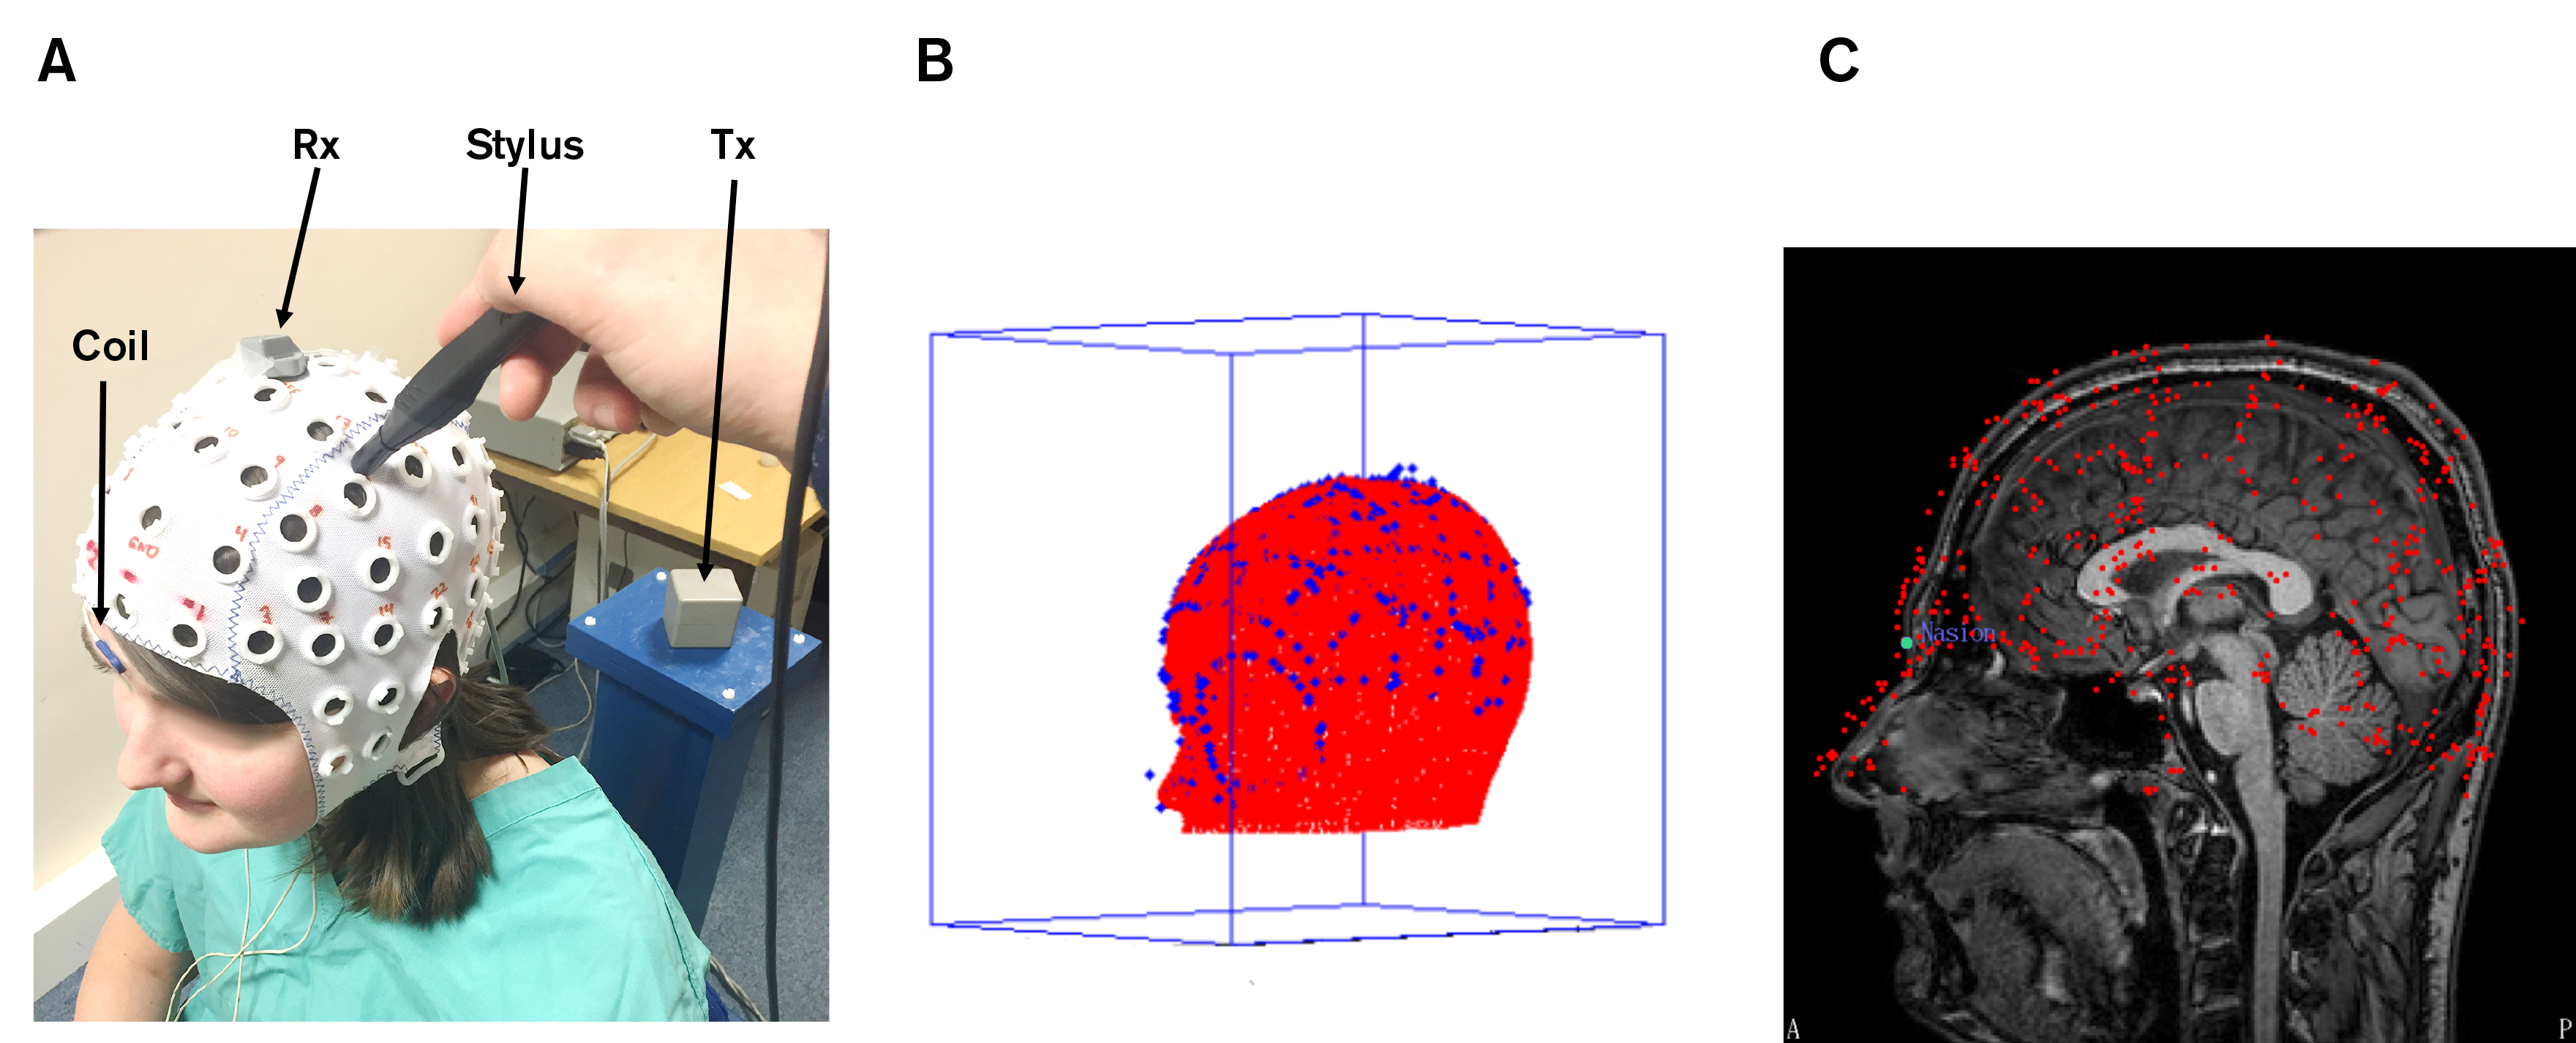
\includegraphics[width=\linewidth]{./images/chapter1/coreg.png}\caption{Data coregistration procedure. A) Digitisation of the head surface using the Polhemus ISOTRAK. B) The digitised head surface (blue dots) are aligned to a head surface derived from an MRI of the participant. C) The result of coregistration, the green dot represents the derived location of the nasion head position indicator. }\label{fig_1_a3}
	\end{center}
\end{figure}

\section*{Summary}

In this chapter a brief overview on the origins on the MEG signal has been given, and the theoretical and practical aspects of data acquisition in a MEG experiment were explained. We have seen that it is possible to measure the extracranial magnetic field associated with dendritic current flow using SQUIDs and that even though they are several orders of magnitude weaker than other sources of interference, it is possible to remove many of these noise sources to be left with data which is a better representative of what is truly inside the sensor dome of the MEG. In the next chapter we move on to discuss how we can reconstruct the sensor data from MEG to derive 3D images of brain current.
\setstretch{1.0}
\chapter{From Sensor to Source: Forward and Inverse Solutions}\label{chapter_meg_source}

In this chapter the fundamental principles of source space reconstruction of MEG sensor data are covered briefly. Whilst not exhaustive, this chapter introduces the generative model of the brain, which provides us with a basis for source reconstruction. In addition, the mathematical framework of the forward and inverse solutions is laid out for use in later chapters in this thesis, with particular focus on spatial filtering techniques. Finally, an investigation into whether the choice of inverse solution has a profound effect on the results of an established functional connectivity pipeline is described. 

\doublespacing
\section*{Introduction}
The magnetic fields that form the basis of MEG are measured using $\sim$300 discrete detectors placed  $\sim$2-4cm from the scalp surface. It is possible to undertake functional connectivity analysis in “sensor space” via assessment between signals measured at separate detectors. However, this comes with three distinct disadvantages:

\begin{enumerate}
	\item \textbf{Field Spread:} The spatial extent of magnetic fields around a current dipole means that multiple sensors will detect signals from a single source which could be erronously interpreted as connections between channels (note this analogous to volume conduction in EEG). \citep{Nunez2006,Scoffelen2009}.
	\item \textbf{Signal Superposition:} A single MEG sensor records a complex mixture of signals generated by many sources, making connectivity assessment between sensors difficult to interpret.
	\item \textbf{Interference:} The magnetic fields generated by the brain are smaller than those generated by external environmental interference (e.g. 50/60 Hz mains electricity). In addition, biological interference, for example from a subject's heart, is larger than the neuromagnetic fields of interest. Interference typically affects many MEG sensors, and hence is highly likely to artificially increase functional connectivity when it is calculated as statistical dependency between sensors. 
\end{enumerate}

The limitations with sensor space analysis are well documented \citep{Scoffelen2009}. Whilst highly successful and meaningful connectivity analyses have been undertaken in this way \citep{Stam2004,Bassett2006,Liu2010}, the inference is usually based on a global parameter (i.e. an integrated measure of global connectivity collapsed across all possible sensor pairs). This means that sensor analysis provides only limited means of interpreting precisely which brain regions or networks are involved. The most successful means to ameliorate the confounds of sensor based connectivity analysis is to apply source space modelling \citep{Scoffelen2009}. This essentially involves mathematically reconstructing the timecourses of electrical activity across many locations (voxels \citep{Hipp2012} or parcellated regions \citep{Hillebrand2012,Tewarie2014a}) in the brain prior to assessment of connectivity between signals reconstructed at those locations. Despite the fact that this projection is mathematically ill posed \citep{Hadamard1902}, there now exists verifiable ways by which to achieve accurate spatial localisation of neural sources, through the use of electromagnetic phantoms (typically supplied with MEG systems for calibration checks routine maintenance) it is possible to test the accuracy of many inverse solutions, for reconstruction of distributed sources and potentially for mapping functional connections. 

In this chapter, we review the theory behind the algorithms which attempt to localise neuronal sources in the brain using extracranial sensor data. Section \ref{sec_gen_model} begins by describing mathematically the generative model which these algorithms attempt to solve. Section \ref{sec_forward_problemn} introduces the forward models used to describe the magnetic field patterns seen on sensor arrays. Section \ref{sec_inverse_problem} introduces the algorithms required to project the data back into source space and finally in Section \ref{sec_bf_v_mn} we present experimental work conducted (by the author) to investigate what effect the choice of inverse solution has on functional connectivity analysis. 

\section{A Generative Model of Sources}\label{sec_gen_model}
The brain contains many possible sources of current dipoles. The measured magnetic fields  outside the head, $\mathbf{b}(t)$, an $n$ element column vector where $n$ is the number of sensors in a system, are the superposition of all the fields generated from the dipoles within the brain volume, $V$ such that,

\begin{equation}
\mathbf{b}(t) = \int_V \mathbf{l}_\mathbf{\theta}q_\mathbf{\theta}(t) dV, \label{eqn_gen_model_1}
\end{equation} where $\mathbf{l}_{\mathbf{\theta}}$ are the lead fields, a model of the magnetic fields for a dipole of unit strength for a given position and orientation vector $\mathbf{\theta}$, and $q_{\mathbf{\theta}}$ is the corresponding dipole strength. Note that it is assumed throughout this thesis, that the lead fields for a source are independent of time, and source orientation is assumed to be constant throughout an experiment. If the brain volume is discretised into a series of $M$ voxels and we assume that only one dipole exists per voxel, we can form the summation

\begin{equation}
\mathbf{b}(t) = \sum_{m=1}^M\mathbf{l}_{\mathbf{\theta}_m}q_{\mathbf{\theta}_m}(t),
\label{eqn_gen_model_2}
\end{equation} it is then possible to introduce a set of composite lead field and dipole vectors:

\begin{equation}
	\begin{aligned}
		\mathbf{L}_V &= 
		\begin{bmatrix} 
			\mathbf{l}_{\mathbf{\theta}_1} & \mathbf{l}_{\mathbf{\theta}_2} & \hdots & \mathbf{l}_{\mathbf{\theta}_M}
		\end{bmatrix},\\
		\mathbf{q}_V(t) &= 
		\begin{bmatrix} 
			q_{\mathbf{\theta}_1}(t) \\ q_{\mathbf{\theta}_2}(t) \\ \vdots \\ q_{\mathbf{\theta}_M}(t)
		\end{bmatrix},
	\end{aligned}	
\end{equation} where $\mathbf{L}_V$ is a $n \times M$ (sensors $\times$ voxels) matrix containing all the information on how the dipoles map to all sensors, and for a given point in time $\mathbf{q}_V(y)$ is a $M\times1$ vector with all the instantaneous dipole strengths. The generative model can now be explained in terms of matrices:

\begin{equation}
\mathbf{b}(t) = \mathbf{L}_V\mathbf{q}_V(t). \label{eqn_gen_model_3}
\end{equation} Note that Equations \ref{eqn_gen_model_1}, \ref{eqn_gen_model_2} and \ref{eqn_gen_model_3} are all equivalent to each other, just expressed differently. 

\section{Estimating the Lead Fields: The Forward Problem}\label{sec_forward_problemn}
To determine the lead fields in Equation \ref{eqn_gen_model_3}, the forward problem needs addressing, which asks: \emph{for a known distribution of current dipoles in the brain, can the associated field pattern be determined?}  Because the magnetic permeability of the head is approximately similar to that of free space ($\mu_r=1$) we can simplify the forward models by treating the entire medium as homogeneous. It is therefore possible to model these dipolar patterns if only the geometric properties of the space between the source and sensor are known. This is in contrast to forward modelling in EEG, as the conductive properties of the skull mean that electric potentials are distorted on detection, meaning complex (and computationally expensive) numerical models such as boundary element models (BEMs) are required.

\subsection{Single Sphere Model}

A model to explain the magnetic field patterns from a source in the brain was developed by \cite{Sarvas1987} and is still the basis of many modern source analyses. The model explains what the field pattern outside a conductive volume would look like if the current is modelled as a dipole within. The electromagnetic fields arising from a bioelectric source with current density $\mathbf{J}$ in a volume $G$ with a constant conductivity $\sigma$ bound by a surface $S$, can be modelled with Maxwell's equations:

\begin{equation}
	\begin{aligned}
		\mathbf{\nabla}\cdot\mathbf{E} &= \frac{\rho}{\epsilon}, \\
		\mathbf{\nabla}\cdot\mathbf{B} &= 0, \\
		\mathbf{\nabla}\times\mathbf{E} &= -\frac{\partial\mathbf{B}}{\partial t}, \\
		\mathbf{\nabla}\times\mathbf{B} &= \mu_0\bigg(\mathbf{J}+\frac{\partial\mathbf{E}}{\partial t}\bigg),
	\end{aligned}\label{eqn_sarvas1}
\end{equation} where $\mu$ and $\epsilon$ are the permeability and permittivity of a medium respectively and $\rho$ is the charge density. As the electromagnetic fields from the brain vary in time at low frequencies (typically < 100 Hz), they are said to be quasi-static (\citealp{Hamalainen1993}; $\frac{\partial}{\partial t}X = 0$, where $X$ is a general function). With this considered, Equation \ref{eqn_sarvas1} can be modified:

\begin{figure}
	\begin{center}
		\includegraphics[width=\linewidth]{./images/chapter2/Figure_1.png}
		\caption{An illustration of the single sphere model with a dipole \textbf{Q} at location \textbf{r}\textsubscript{Q}. The spherical volume conductor, G bounded by a spherical surface, S. A detector is placed at location \textbf{r} and we consider the fictitious current (which is non existent, but aids the mathematical analysis) at \textbf{r}'. \label{figure_2_1}}
	\end{center}
\end{figure}

\begin{equation}
	\begin{aligned}
	%\mathbf{E} &= -\mathbf{\nabla}V,\\
	\mathbf{\nabla}\times\mathbf{E} &= 0, \\
	\mathbf{\nabla}\times\mathbf{B} &= \mu_0\mathbf{J}, 
	\end{aligned}\label{eqn_sarvas1a}
\end{equation} Given that $\mathbf{J}$ is the total current density then $\mathbf{B}$ is given by the Ampére-Laplace law:

\begin{equation}
\mathbf{B}(\mathbf{r}) = \frac{\mu_0}{4\pi}\int_{G}\mathbf{J}(\mathbf{r}')\times\frac{\mathbf{r}-\mathbf{r}'}{|\mathbf{r}-\mathbf{r}'|^3}\text{d}\nu', \label{eqn_sarvas2}
\end{equation} where $\mathbf{r}'$ represents a location of a dipole in the volume $G$, $\mathbf{r}$ is a location outside of the volume (as shown in Figure \ref{figure_2_1}) and $\text{d}\nu'$ is a volume element. For a post-synaptic current we can define the current density as

\begin{equation}
\begin{aligned}
\mathbf{J}_\text{PS} &= \mathbf{J}^P+\mathbf{J}^V \\
&= \mathbf{J}^P - \sigma\mathbf{\nabla}V \label{eqn_2_8}
\end{aligned}
\end{equation} where $\mathbf{J}^P$ and $\mathbf{J}^V = - \sigma\mathbf{\nabla}V$ are the primary and volume current densities respectively (see Figure \ref{fig_1_b2}). By defining $\mathbf{R} = \mathbf{r}-\mathbf{r}'$ by substituting Equation \ref{eqn_2_8} into \ref{eqn_sarvas2} we can define $\mathbf{B}$ in terms of the primary and volume currents of a dendrite: 

\begin{equation}
	\begin{aligned}
		\mathbf{B}(\mathbf{r}) &= \frac{\mu_0}{4\pi}\int_{G}\Big(\mathbf{J}^P(\mathbf{r}')-\sigma\mathbf{\nabla}V(\mathbf{r}')\Big)\times\frac{\mathbf{R}}{|\mathbf{R}|^3}\text{d}\nu' \\
		&= \frac{\mu_0}{4\pi}\int_{G}\mathbf{J}^P(\mathbf{r}')\times\frac{\mathbf{R}}{|\mathbf{R}|^3}\text{d}\nu' - \frac{\mu_0\sigma}{4\pi}\int_{G}\mathbf{\nabla}V(\mathbf{r}')\times\frac{\mathbf{R}}{|\mathbf{R}|^3}\text{d}\nu'. \label{eqn_amplaplace}
	\end{aligned}
\end{equation} Here, the first term represents the contribution of the primary current to the magnetic field, and is invariant to conductivity. Briefly, we focus on the term which corresponds to the volume current: 

\begin{equation}
\mathbf{B}^V(\mathbf{r}) = - \frac{\mu_0\sigma}{4\pi}\int_{G}\mathbf{\nabla}V(\mathbf{r}')\times\frac{\mathbf{R}}{|\mathbf{R}|^3}\text{d}\nu',
\label{eqn_volume_magentic_field}
\end{equation}if we recall the vector identity $\mathbf{\nabla}a\times\mathbf{\nabla}b = \mathbf{\nabla}\times(a\mathbf{\nabla}b)$, and assume $\mathbf{\nabla}a=\mathbf{\nabla}V$ and $\mathbf{\nabla}b = \mathbf{R}|\mathbf{R}|^{-3}$, we can rewrite Equation \ref{eqn_volume_magentic_field} so that

\begin{equation}
\mathbf{B}^V(\mathbf{r}) = - \frac{\mu_0\sigma}{4\pi}\int_{G}\mathbf{\nabla}\times V(\mathbf{r}')\frac{\mathbf{R}}{|\mathbf{R}|^3}\text{d}\nu'. \label{eqn_stokes} 
\end{equation} Next, we recall the generalised Stokes theorem 

\begin{equation}
	\int_G\mathbf{\nabla}\times\mathbf{X}\text{d}\nu'=\int_S\mathbf{n}\times\mathbf{X}\text{d}s 
\end{equation} where \textbf{n} is a vector normal to the surface element $\text{d}s$ (directed outwards from the volume centre). Combining Equations \ref{eqn_amplaplace}, \ref{eqn_volume_magentic_field} and \ref{eqn_stokes} we arrive at a new expression for \textbf{B}(r):

\begin{equation}
\begin{aligned}
	\mathbf{B}(\mathbf{r}) &= \frac{\mu_0}{4\pi}\int_{G}\mathbf{J}^P(\mathbf{r}')\times\frac{\mathbf{R}}{|\mathbf{R}|^3}\text{d}\nu' - \frac{\mu_0\sigma}{4\pi}\int_SV(\mathbf{r}')\mathbf{n}(\mathbf{r}')\times\frac{\mathbf{R}}{|\mathbf{R}|^3}\text{d}s \\ 
	&= \mathbf{B}_0(\mathbf{r}) - \frac{\mu_0\sigma}{4\pi}\int_SV(\mathbf{r}')\mathbf{n}(\mathbf{r}')\times\frac{\mathbf{R}}{|\mathbf{R}|^3}\text{d}s,
	\label{eqn_geselowitz}
	\end{aligned}
\end{equation} Equation \ref{eqn_geselowitz} is a modified version of the Geselowitz formula \citep{Geselowitz1970}, which states that the volume current can be represented as a set of fictitious currents (non existent currents which aid the mathematical formulation) flowing on a conductive surface, \textit{S}. Physically, such currents are non existent but otherwise prove useful for further calculations. If we now assume the volume \textit{G} to be bound within a spherical surface \textit{S}, and that the MEG system can only detect the radial component of a magnetic field such that:
\begin{equation}
\begin{aligned}
B_r(\mathbf{r}) &= \mathbf{B}(\mathbf{r})\cdot\mathbf{e}_r \\
& = \frac{\mu_0}{4\pi}\int_{G}\mathbf{J}^P(\mathbf{r}')\times\frac{\mathbf{r}-\mathbf{r}'}{|\mathbf{r}-\mathbf{r}'|^3}\cdot\mathbf{e}_r\text{d}\nu' - \frac{\mu_0\sigma}{4\pi}\int_SV(\mathbf{r}')\mathbf{n}(\mathbf{r}')\times\frac{\mathbf{r}-\mathbf{r}'}{|\mathbf{r}-\mathbf{r}'|^3}\cdot\mathbf{e}_r\text{d}s
\end{aligned}
\end{equation} where $\mathbf{e}_r$ is the unit vector normal to the plane of a MEG sensor. Focussing on a term in the surface integral:

\begin{equation}
\begin{aligned}
 \mathbf{n}(\mathbf{r}')\times(\mathbf{r}-\mathbf{r}')\cdot\mathbf{e}_r &= \Big(\mathbf{n}(\mathbf{r}')\times\mathbf{r}-\underset{\parallel}{\underbrace{\mathbf{n}(\mathbf{r}')\times\mathbf{r}'}}\Big)\cdot\mathbf{e}_r \\
 &=\underset{\perp}{\underbrace{\mathbf{n}(\mathbf{r}')\times\mathbf{r}\cdot\mathbf{e}_r}} \\
 &=0
 \end{aligned} 
\end{equation} means that the surface integral term vanishes, leaving an expression for $B_r$ which is not dependent on the volume currents and crucially, invariant to conductivity:

\begin{equation}
	\begin{aligned}
		B_r(\mathbf{r}) &= \frac{\mu_0}{4\pi}\int_{G}\mathbf{J}^P(\mathbf{r}')\times\frac{\mathbf{r}-\mathbf{r}'}{|\mathbf{r}-\mathbf{r}'|^3}\cdot\mathbf{e}_r\text{d}\nu'. \\
		&= \mathbf{B}_0(\mathbf{r})\cdot\mathbf{e}_r
		\label{eqn_Br_no_conduction}
	 \end{aligned}
\end{equation} Now, we introduce the idea that current from a dipole is not equally distributed across the volume, but rather exists at a single point in space (\textbf{r}\textsubscript{Q}) as a current dipole, 

\begin{equation}
\mathbf{J}^P(\mathbf{r}') = \mathbf{Q}\delta(\mathbf{r}'-\mathbf{r}_Q),
\end{equation} where \textbf{Q} represents the magnitude and direction of the dipole and $\delta$ is the Dirac delta function. Using this allows us to simplify the integral in Equation \ref{eqn_Br_no_conduction}

\begin{equation}
\begin{aligned}
B_r(\mathbf{r}) &= \frac{\mu_0}{4\pi}\int_{G}\mathbf{Q}\delta(\mathbf{r}'-\mathbf{r}_Q)\times\frac{\mathbf{r}-\mathbf{r}'}{|\mathbf{r}-\mathbf{r}'|^3}\cdot\mathbf{e}_r\text{d}\nu' \\
&= \frac{\mu_0}{4\pi} \mathbf{Q}(\mathbf{r}_Q)\times\frac{\mathbf{r}-\mathbf{r}_Q}{|\mathbf{r}-\mathbf{r}_Q|^3}\cdot\mathbf{e}_r \\
%&= \frac{\mu_0}{4\pi} \Bigg(\frac{\mathbf{Q}(\mathbf{r}_Q)\times\mathbf{r}\cdot\mathbf{e}_r}{|\mathbf{r}-\mathbf{r}_Q|^3} - \frac{\mathbf{Q}(\mathbf{r}_Q)\times\mathbf{r}_Q\cdot\mathbf{e}_r}{|\mathbf{r}-\mathbf{r}_Q|^3} \Bigg) \\
%&= -\frac{\mu_0}{4\pi}\frac{\mathbf{Q}\times\mathbf{r}_Q\cdot\mathbf{e}_r}{|\mathbf{r}-\mathbf{r}_Q|^3}
\end{aligned}
\end{equation} To calculate the other components of the magnetic field outside the volume, we note that $\mathbf{J}=0$ outside of $G$ and therefore according to Equation \ref{eqn_sarvas1a}, $\mathbf{\nabla}\times\mathbf{B} = 0$, allowing us to express the magnetic field in terms of the magnetic scalar potential, $U$:

\begin{equation}
	\mathbf{B}(\mathbf{r}) = -\mu_0\mathbf{\nabla}U(\mathbf{r}). \label{eqn_pot_formula}
\end{equation} To determine an expression for $U$, we need to fix \textbf{r} to be outside of $G$ and consider a line integral of $\mathbf{\nabla}U$ along the radius of $G$, $0 \leq t \leq \infty$. As $U$ is a vanishing term at infinity, we obtain

\begin{equation}
	\begin{aligned}
		U(\mathbf{r}) &= - \int_0^\infty \mathbf{\nabla}U(\mathbf{r}+t\mathbf{e}_r)\cdot\mathbf{e}_r\text{d}t \\
		&= \frac{1}{\mu_0}\int_0^\infty B_r(\mathbf{r}+t\mathbf{e}_r)\text{d}t \\
		&= \frac{1}{\mu_0}\int_0^\infty \mathbf{B}_0(\mathbf{r}+t\mathbf{e}_r)\cdot\mathbf{e}_r\text{d}t \\
		&= \frac{1}{4\pi}\mathbf{Q}\times(\mathbf{r}-\mathbf{r}_Q)\cdot\mathbf{e}_r \int_0^\infty{\frac{\text{d}t}{|\mathbf{r}+t\mathbf{e}_r-\mathbf{r}_Q|^3}}.
	\end{aligned}
\end{equation} Solving the integral gives us

\begin{equation}
	U(\mathbf{r}) = -\frac{1}{4\pi}\frac{\mathbf{Q}\times\mathbf{r}_Q\cdot\mathbf{r}}{F} \label{eqn_pot_solution}
\end{equation} where 

\begin{equation}
F = |\mathbf{a}|\Big(|\mathbf{r}||\mathbf{a}|+|\mathbf{r}|^2-(\mathbf{r}_Q\cdot\mathbf{r})\Big) \label{eqn_F}
\end{equation} and $\mathbf{a}=\mathbf{r}-\mathbf{r}_Q$. Note that $U(\mathbf{r})$ and thus, \textbf{B} outside of $G$ is not dependent on the conductivity profile of the volume. Inserting Equations \ref{eqn_pot_solution} and \ref{eqn_F} into Equation \ref{eqn_pot_formula} gives us a final expression for the magnetic field.

\begin{equation}
\mathbf{B}(\mathbf{r})=\frac{\mu_0}{4\pi F^2}(F\mathbf{Q}\times\mathbf{r}_Q-\mathbf{Q}\times\mathbf{r}_Q\cdot\mathbf{r\nabla}F) \label{eqn_sarvas_final}
\end{equation} where

\begin{equation}
\mathbf{\nabla}F = \Bigg(\frac{|\mathbf{a}|^2}{|\mathbf{r}|}+\frac{\mathbf{a}}{|\mathbf{a}|}\cdot\mathbf{r}+2|\mathbf{a}|+2|\mathbf{r}|\Bigg)\mathbf{r}
-\Bigg(|\mathbf{a}|+2|\mathbf{r}|+\frac{\mathbf{a}}{|\mathbf{a}|}\cdot\mathbf{r}\Bigg)\mathbf{r}_Q
\end{equation} Equation \ref{eqn_sarvas_final} is known as the Sarvas equation and is the general solution to the single sphere model. An important property of this equation is that if a dipole is radially oriented in a spherical conductor, then the magnetic field outside of it vanishes. However the cortical sulci are folded such that many of the neuronal ensembles ($\sim$70\%) have a detectable tangential component \citep{Hillebrand2002}. 

\subsection{Multiple Spheres Model}
Whilst the single sphere model can quickly explain the magnetic fields outside of the body, it grossly simplifies the geometry of the head. Large areas of the brain which deviate from spherical geometry such as the frontal and fronto-temporal regions find the single sphere inadequate \citep{Hamalainen1989}. In 1999, Huang and colleagues built upon the single sphere model further and devised a system of generating a series of overlapping spheres, known as the multiple or local sphere model \citep{Huang1999}. For every sensor, a sphere is generated and placed in the vicinity of the sensor, such that it fits within the geometry of the skull. Repeating for each sensor results in a series of homogeneous overlapping spheres with a geometry which better approximates the brain. The lead fields can then be estimated from a combination of all the spheres (and thus multiple applications of Equation \ref{eqn_sarvas_final}). In a comparison between the single sphere, multiple spheres and a three shell BEM, the multiple spheres model was in better agreement with the BEM than the single sphere model. In particular, the frontal and visual regions (which deviate the most from a sphere) where better reconstructed. The key advantage of the local spheres model over the BEM is that it can be utilised at a fraction of the computational cost. It is for this reason that a multiple spheres head model is used as the forward model for all investigations in this thesis.

\subsection{Single Shell Model}
Another forward field solutions which has gained popularity recently is that of using a spherical harmonic basis set to approximate the head \citep{Nolte2003}. The premise is that head is assumed to be a homogeneous single volume with an isotropic conductivity profile and so the single sphere model can be expanded such that lead field at a position \textbf{r} is

\begin{equation}
\mathbf{L}(\mathbf{r}) = \mathbf{L}(\mathbf{r})_\text{sphere} - \mathbf{\nabla}U(\mathbf{r})
\end{equation} where $\mathbf{L}(\mathbf{r})_\text{sphere}$ are the lead field based on the single sphere approximation of the head, and $U(\mathbf{r})$ is a spherical harmonic basis set, chosen such that the lead fields will be tangential at the surface of the volume conductor. The model increases with accuracy with more harmonics added, with Nolte recommending 20, however this comes at the cost of computational efficiancy. In a comparison of the aforementioned forward solutions with high polygon BEMs, \cite{Stenroos2014} found that the single shell model performs considerably better than either of the single sphere or multiple sphere approaches, with near parity to a 3-shell BEM. 

\section{Source Reconstruction: The Inverse Problem}\label{sec_inverse_problem}
Having now estimated the lead fields, attention turns to inferring the underlying neural activity by inverting the generative model. The inverse problem asks: \textit{if you have a series of magnetic field measurements from an array, can the location of the underlying current source be determined}? Whilst this question appears initially similar to the forward problem it is non-trivial for a number of reasons:

\begin{enumerate}
	\item{The number of potential source locations in the brain greatly outnumbers the recordings.}
	\item{The linear superposition of electromagnetic fields means that adjacent sources may cancel each other out, silent sources such as radially oriented dipoles or closed loops mean there are an infinite number of solutions.}
	\item{Magnetic fields travel at the speed of light, so propagate to all channels without there being a measurable lag in time between sensors. }
\end{enumerate} With this in mind knowing the exact lead fields corresponding to a location of interest is not sufficient, and extra assumptions have to be made. The simplest solution would be to fit a dipole which matches the field patterns seen on the sensor level, but this is limited to the assumption that the brain will only have a \textit{a-priori} determined number of dipoles activated at any given moment (typically only a few). For connectivity analysis across large regions of brain, this is insufficient and solutions which can accommodate many distributed sources are required.  

\subsection{The Generalised Minimum Norm Solution}
The earliest solution to the inverse problem for many neural sources was proposed by Hamalainen and colleages in 1984 \citep{Hamalainen1994}, which involves minimising the L2 norm of the discrepancy between the measured data $\textbf{b}(t)$ and the model of the source data $\hat{\mathbf{b}}(t)$. Recalling the most general case in Equation \ref{eqn_gen_model_1}:
\begin{equation}
\underset{\hat{q}_\mathbf{\theta}}{\text{min}}\left\| \textbf{b}(t)-\int_V \mathbf{l}_\mathbf{\theta}\hat{q}_\mathbf{\theta}(t) dV\right\|^2_2.\label{eqn_gmn1}
\end{equation} If we assume discretisation and recall Equation \ref{eqn_gen_model_3}, Equation \ref{eqn_gmn1} can be rewritten as

\begin{equation}
\underset{\hat{\mathbf{q}}_V(t)}{\text{min}}\left\| \textbf{b}(t)-\mathbf{L}_V\hat{\mathbf{q}}_V(t)\right\|^2_2,
\end{equation} where $\hat{\mathbf{q}}_V$ represents the estimated instantaneous source amplitudes for all dipoles across voxels. It is important to note there by discreitsing the source space, we have simplified the analysis (and computing power to solve) considerably, but have introduced error by undersampling (much akin to using the trapezium rule to solve an integral or the Euler discretisation method to solve an ordinary differential equation). To solve for $\hat{\mathbf{q}}_V$ it would appear to be appropriate to rearrange Equation \ref{eqn_gen_model_3} to form $\mathbf{q}_V(t) = \mathbf{L}_V^{-1}\mathbf{b}(t)$, however  $\mathbf{L}_V$ is generally not square, and therefore is not invertable. Instead we recall Equation \ref{eqn_gen_model_3} and multiply both sides by $\mathbf{L}_V^T$ such that

\begin{equation}
\begin{aligned}
\mathbf{L}_V^T\mathbf{b}_V(t) &= \mathbf{L}_V^T\mathbf{L}_V \mathbf{q}_V(t)	\\
\hat{\mathbf{q}}_V(t) &= \mathbf{L}_V^T\mathbf{b}_V(t)\big[\mathbf{L}_V^T\mathbf{L}_V\big]^{-1} \\
&= \mathbf{L}_V^+\mathbf{b}_V(t), \\
\end{aligned} \label{eqn_MN_1a}	
\end{equation} where $\mathbf{L}_V^T = \mathbf{L}_V^T\big[\mathbf{L}_V\mathbf{L}_V^T\big]^{-1}$, the Moore-Penrose pseudoinverse of $\mathbf{L}_V$, which is square. The term in the bracket is the $n \times n$ inner product of all the calculated lead fields across the entire brain volume, and is known as the Gram matrix $(\mathbf{G} = \mathbf{L}_V\mathbf{L}_V^T)$. We can rewrite Equation \ref{eqn_MN_1a} as 

\begin{equation}
		\hat{\mathbf{q}}_V(t) = \mathbf{L}^T_V\mathbf{G}^{-1} \mathbf{b}(t).	
	\label{eqn_2_26}	
\end{equation} $\mathbf{G}$ may be square, but is not necessarily invertible as it may be (or be close to) singular, resulting in the introduction of numerical errors on inversion\footnote{The definition of a singular matrix is if (and only if) the determinant of the matrix is exactly 0, which is unlikely to happen in practice. Rather, the determinant of \textbf{G} is likely be very low ($<<$ 1). So while \textbf{G} can \textit{technically} be inverted, the solution and hence source reconstruction will be so unstable that an alternative expression of \textbf{G} must be found.}. To overcome the problems with finding $\mathbf{G}^{-1}$, Tikhonov regularisation \citep{Tikhonov1943} is employed to stabilise $\mathbf{G}$. The regularised Gram matrix is defined as 
\begin{equation}
\mathbf{G}_r = (\mathbf{G}+\mu\mathbf{I}),
\end{equation} where $\mu$ is a scalar parameter and $\mathbf{I}$ is an identity matrix the same size as $\mathbf{G}$. By adding $\mu$ to the leading diagonal, all eigenvalues of $\mathbf{G}_r$ will be non-zero, thus no longer a singular matrix. Equation \ref{eqn_2_26} can be rewritten as:

\begin{equation} \label{eqn_MN_general}
\hat{\mathbf{q}}_V(t) = \mathbf{L}_V^{T}(\mathbf{G}+\mu\mathbf{I})^{-1} \mathbf{b}(t),
\end{equation} which is the solution to the cost function \citep{Sekihara2008}

\begin{equation}
\underset{\hat{\mathbf{q}}_V(t)}{\text{min }} \big(\underbrace{\left\| \textbf{b}(t)-\mathbf{L}_V\hat{\mathbf{q}}_V(t) \right\|^2_2}_{\substack{\text{difference between} \\\text{data and model}}} + \underbrace{\mu\left\| \hat{\mathbf{q}}_V(t) \right\|^2_2}_{\substack{\text{measurement of the} \\\text{total power across} \\\text{the brain}}} \big),
\end{equation} meaning that both the total power across the brain and model error are minimised. The regularisation parameter $\mu$ is the variable which trades off between these two terms. Increasing $\mu$ means that the power (therefore the noise), but at the cost of reducing the error in the model, which leads to spatial smearing of the localised sources. Equation \ref{eqn_MN_general} is the general Minimum Norm solution upon which all variants are built.

\subsection{Minimum Norm Spatial Filter}
In order to be able to compare this inverse solution with other variants, it is convenient to investigate the current at a single \textit{a-priori} selected region, rather than consider source behaviour over the entire brain volume simultaneously. The basis of spatial filtering is to reconstruct the electrical timecourse $\hat{\mathbf{q}}_\mathbf{\theta}(t)$ at a given location and orientation $\mathbf{\theta}$. A graphical description of spatial filtering can be found in Figure \ref{figure_2_3}, but a mathematical description hereby follows. The typical method to reconstruct the current at $\mathbf{\theta}$ is to calculate a linear weighted sum of the sensor measurements such that

\begin{equation}\label{eqn_filter_gen}
	\begin{aligned}
		\hat{\mathbf{q}}_\mathbf{\theta}(t) &= w_{\mathbf{\theta}_1}b_1(t) + w_{\mathbf{\theta}_2}b_2(t) + \ldots + w_{\mathbf{\theta}_n}b_n(t) \\
		&= \mathbf{w}^T_\mathbf{\theta}\mathbf{b}(t).
	\end{aligned}
\end{equation}

Equation \ref{eqn_filter_gen} is the general solution to most spatial filters and it is important to note that the majority of electrophysiological inverse solutions can be formulated in this way, with how $ \mathbf{w}_\mathbf{\theta}$ is derived differentiating methods. In the case of minimum norm solutions, Equation \ref{eqn_MN_general} can be rewritten on a voxel-by-voxel basis as

\begin{equation}
		\begin{bmatrix} 
		\hat{q}_{\mathbf{\theta}_1}(t) \\ \hat{q}_{\mathbf{\theta}_2}(t) \\ \vdots \\ \hat{q}_{\mathbf{\theta}_M}(t)
		\end{bmatrix} = 
		\begin{bmatrix} 
		\mathbf{l}^T_{\mathbf{\theta}_1} \\ \mathbf{l}^T_{\mathbf{\theta}_2} \\ \vdots \\ \mathbf{l}^T_{\mathbf{\theta}_M}
		\end{bmatrix}\mathbf{G}^{-1}_r\mathbf{b}(t),
\end{equation} where $\mathbf{l}_{\mathbf{\theta}}$ is a $N \times 1$ vector and represents the lead fields for a given $\mathbf{\theta}$. For a single voxel, the spatial filter can be defined as

\begin{equation}
	\hat{q}_\mathbf{\theta}(t) = \mathbf{l}_\mathbf{\theta}^T\mathbf{G}_r^{-1}\mathbf{b}(t).
\end{equation} Given the general definition of the spatial filter in Equation \ref{eqn_filter_gen} the weights of the Minimum Norm spatial filter for a given $\mathbf{\theta}$ are
\begin{equation}\label{eqn_weights_mn}
	\mathbf{w}_{\mathbf{\theta}_{MN}}^T = \mathbf{l}^T_\mathbf{\theta}\mathbf{G}^{-1}_r.  
\end{equation}  
	
\begin{figure}[h!]
	\begin{center}
		\includegraphics[width=0.8\linewidth]{./images/chapter2/Figure_2.png}
		\caption{A diagram to illustrate the concept of spatial filtering. A source $\mathbf{q_\theta}$ in the brain can be represented as the weighted sum of the extracranial mesurements from an MEG sensor array. The weights of each sensor in this diagram may, for example, scale with distance, represented by the darkness of the arrows representing $w$.\label{figure_2_3}}
	\end{center}
\end{figure}

\subsection{Beamforming}

Beamforming is an alternative approach to spatial filtering which has become a popular alternative to minimum norm estimations, particularly in the imaging of the spatial signature of neural oscillations. First developed for RADAR in World War II,  beamforming was introduced to MEG by \cite{Robinson1992}.

Beamforming starts with the same spatial filter formulation in Equation \ref{eqn_filter_gen}, but instead $\mathbf{w_\theta}$ is based on power minimisation. In particular the output of the beamformer $\hat{q}_\mathbf{\theta}(t)$ is minimised with the constraint that the power at $\mathbf{\theta}$ remains unchanged. If the estimated power is defined as the expectation value of the squared signal 

\begin{equation} \label{eqn_bf_2}
P_{\mathbf\theta} = \big\langle\hat{q}^2_{\mathbf\theta}(t)\big\rangle,
\end{equation}
then the beamformer can be formulated mathematically as 

\begin{equation} \label{eqn_bf_3}
\underset{\mathbf{w_\theta}}{\text{min }}\big(\langle\hat{q}^2_{\mathbf\theta}(t)\rangle\big)\text{, subject to } \mathbf{w}_{\mathbf{\theta}}^T\mathbf{l_\theta} = 1.
\end{equation}
Note that the linear constraint  $\mathbf{w_\theta}^T\mathbf{l_\theta} = 1$ comes from the definition of the lead field model of a unit dipole, meaning power remains at unity. Substituting Equation \ref{eqn_filter_gen} into Equation \ref{eqn_bf_2} gives

\begin{equation}
\begin{aligned}\label{eqn_bf_4}
P_{\mathbf\theta} &= \Big\langle \big(\mathbf{w}^T_{\mathbf\theta}\mathbf{b}(t)\big)\big(\mathbf{w}^T_{\mathbf\theta}\mathbf{b}(t)\big)^T\Big\rangle \\
&= \mathbf{w}^T_{\mathbf\theta}\big{\langle}\mathbf{b}(t)\mathbf{b}(t)^T\big\rangle\mathbf{w}_{\mathbf\theta}\\
&\approx \mathbf{w}^T_{\mathbf\theta}\mathbf{C}\mathbf{w}_{\mathbf\theta},
\end{aligned}
\end{equation}
where $\mathbf{C}$ is the $n \times n$ data covariance matrix of the magnetic field data recorded by the MEG sensor, where the $ij^{\text{th}}$ element is the covariance of the data recorded at channels $i$ and $j$ respectively. In general, if we want to find the extrema of a function, $f(x)$ with the added linear constraint of $g(x)=0$, we can form a composite function called a Lagrangian such that

\begin{equation}
	\mathscr{L}(x,\lambda) = f(x) + \lambda g(x)
\end{equation} where $\lambda$ is a scalar value called a Lagrange multiplier. We can form a Lagrangian describing the power output of the beamformer based on Equation \ref{eqn_bf_3}:

\begin{equation}\label{eqn_bf_8}
\mathscr{L}(\mathbf{w_\theta},\lambda ) = \mathbf{w}^T_{\mathbf\theta}\mathbf{C}\mathbf{w}_{\mathbf\theta} + \lambda (\mathbf{w_\theta}^T\mathbf{l_\theta} - 1).
\end{equation} To satisfy the conditions set by Equation \ref{eqn_bf_3}, we need to solve $\mathbf{\nabla}\mathscr{L}(\mathbf{w_\theta},\lambda )=0$:

\begin{equation}\label{eqn_bf_9}
\frac{\partial \mathscr{L}(\mathbf{w_\theta},\lambda )}{\partial \mathbf{w_\theta}} = 2\mathbf{C}\mathbf{w}_{\mathbf\theta} + \lambda \mathbf{l_\theta} = 0.
\end{equation} Rearranging Equation \ref{eqn_bf_9} gives an expression of $\mathbf{w_\theta}$ in terms of $\lambda$

\begin{equation}\label{eqn_bf_9a}
\mathbf{w_\theta} = -\lambda\mathbf{C}^{-1}\mathbf{l_\theta}/2.
\end{equation} By equating $\mathbf{w_\theta}^T\mathbf{l_\theta} - 1 = 0$ with Equation \ref{eqn_bf_9} it is possible to give an expression for $\lambda$: 

\begin{equation}\label{eqn_bf_10}
\lambda = -2[\mathbf{l}^T_{\mathbf\theta}\mathbf{C}^{-1}\mathbf{l}_{\mathbf\theta}]^{-1},
\end{equation} substituting Equation \ref{eqn_bf_10} into \ref{eqn_bf_9a}, we arrive a a solution for the beamformer weights:

\begin{equation}\label{eqn_weights_bf}
\mathbf{w}_{\mathbf{\theta}_{BF}}^T = \frac{\mathbf{l_\theta}^T\mathbf{C}^{-1}}{\mathbf{l}^T_{\mathbf\theta}\mathbf{C}^{-1}\mathbf{l}_{\mathbf\theta}}.
\end{equation}Note that whilst $\mathbf{C}$ has not been regularised here, it can be Tikhonov regularised like the Gram matrix $\mathbf{G}$. Here, $\mathbf{C}_r = \mathbf{C} + \eta\mathbf{I}$ where $\eta$ is a scalar parameter and $\mathbf{I}$ is an $n\times n$ identity matrix. 

\subsection{Determining source orientation}\label{sec_334}

A core parameter of a successful source reconstruction is the source orientation. Thus far, we have assumed that the orientation of a source was known, but in practice this is not the case. A correct estimation of these angles is important, as along with source location, orientation has an effect on the weighting parameter, $\mathbf{w}$. Whilst it is known that the sources seen in MEG are unlikely to be radial, it could exist at one of many other orientations. There are two popular approaches to finding the optimal orientation, both of which follow the underlying principle that the best orientation to model is the one which gives the maximal SNR for a given location.

\subsubsection{Exhaustive search method} In this method, the orientation is found from an exhaustive search of all possible orientations. However, as we assume radial sources do not contribute to the MEG, the orientation of a dipole is constrained to remain azimuthal to the surface of the brain, determined from the head model derived from the anatomical image of the subject. Consequently, this reduces the complexity and the size of the search. From here multiple dipoles are modelled, all at different angles of $0 \leq \phi \leq \pi$, where $\phi$ is the azimuthal angle. For every orientation of $\phi$ at a given position \textbf{r}, the corresponding weight vectors are calculated and then a search for the maximal SNR is performed  by measuring the pseudo-Z statistic for each orientation. In the case of a beamformer this is calculated by:

\begin{equation}
\text{\sout{Z}}_{\mathbf{r},\phi} = \frac{\mathbf{w}_{\mathbf{r},\phi}^T\mathbf{C}\mathbf{w}_{\mathbf{r},\phi}}{\mathbf{w}_{\mathbf{r},\phi}^T\mathbf{\Sigma}\mathbf{w}_{\mathbf{r},\phi}},
\end{equation} where $\mathbf{\Sigma} = \sigma^2\mathbf{I}$ is the noise covariance matrix, $\sigma^2$ is the uncorrelated noise power at each MEG sensor and $\mathbf{I}$ is an identity matrix. $\phi$ is determined from the maximum value of $\text{\sout{Z}}_{\mathbf{r},\phi}$ and the corresponding column of weights is selected for reconstruction. This method (for arcane reasons in the Nottingham MEG group) is used to determine source orientation. 

\subsubsection{Eigenvalue decomposition}

An alternative method was proposed by \cite{Sekihara2004}. In an eigenvalue orientation determination the objective is to reconstruct a 3-element dipole timecourse for a given location and find the combination of those three timecourses which gives maximal variance. To achieve this the weights for a given location are calculated in three orthogonal orientations, $[\mathbf{w}_{r_i}, \mathbf{w}_{r_j}, \mathbf{w}_{r_k}]$ and three source timecourses are reconstructed to form  $\mathbf{q}_r = [\mathbf{q}_{r_i}, \mathbf{q}_{r_j}, \mathbf{q}_{r_k}]$. Note that the orientations of $i$, $j$ and $k$ are perpendicular to each other, but otherwise arbitrary. To find the maximal variance, the first principal component of $\mathbf{q}_r$ is calculated, to give a solution which is equivalent to the scalar solution.  

\subsection{Depth correction}\label{sub_depthcorrection}

The problem with the weights derived for minimum norm and beamforming in Equations \ref{eqn_weights_mn} \& \ref{eqn_weights_bf} is that they have a tendency to mislocalise sources. For the minimum norm spatial filter, it tends to bias sources nearer the sensors (i.e it pulls sources towards the outside of the brain \citep{Fuchs1999,Lin2006}) due to attenuation of the lead fields for deeper sources. This has led to the development of a series of "weighted minimum norm" solutions which come in many varieties \citep{Fuchs1999,Dale2000,Pascual-Marqui2002,Lin2006} but all share the same goal of implementing a depth correction step into the source reconstruction. One popular variant, dynamic Statistical Parametric Mapping (dSPM) \citep{Dale2000} attempts to normalise the minimum norm weights by their own norm, ensuring an even noise distribution across the entirety of the brain. 

\begin{equation} \label{eqn_weights_dspm}
	\begin{aligned}
		\mathbf{w}^T_{\mathbf{\theta}_{dSPM}} &= \frac{\mathbf{l}^T_\mathbf{\theta}\mathbf{G}^{-1}}{\big\|\mathbf{w}_{\mathbf{\theta}_{MN}}^T\big\|} \\
		& = \frac{\mathbf{l}^T_\mathbf{\theta}\mathbf{G}^{-1}}{\sqrt{\mathbf{l}^T_\mathbf{\theta}\mathbf{G}^{-2}\mathbf{l}_\mathbf{\theta}}}.
	\end{aligned}
\end{equation} For beamformers the bias is toward the centre of the brain. This occurs due to norm of the lead fields falling towards the centre, which in turn increases the norm of the beamformer weights for deeper sources and increases their variance. Again, this is compensated for by scaling the beamformer weights by their own norm: 

\begin{equation} \label{eqn_weights_z_1}
	\big\|\mathbf{w}_{\mathbf{\theta}_{BF}}\big\| = \frac{\sqrt{\mathbf{l}^T_\mathbf{\theta}\mathbf{C}^{-2}\mathbf{l}_\mathbf{\theta}}}{\mathbf{l}^T_\mathbf{\theta}\mathbf{C}^{-1}\mathbf{l}_\mathbf{\theta}}.
\end{equation} Dividing Equation \ref{eqn_weights_bf} by \ref{eqn_weights_z_1} gives the depth corrected beamformer weights:

\begin{equation} \label{eqn_weights_z_2}
\mathbf{w}^T_{\mathbf{\theta}_{\text{\sout{Z}}}} = \frac{\mathbf{l}^T_\mathbf{\theta}\mathbf{C}^{-1}}{\sqrt{\mathbf{l}^T_\mathbf{\theta}\mathbf{C}^{-2}\mathbf{l}_\mathbf{\theta}}}.
\end{equation} Here the subscript \sout{Z} denotes that the depth corrected bemformer weights do not produce a current dipole with units Am, but instead a pseudo-Z statistic. Note there is a direct equivalence between equations \ref{eqn_weights_dspm} and \ref{eqn_weights_z_2} \citep{Mosher2003}. The difference between the two reconstruction methods boils down to one being data driven (the data covariance in beamforming) and one being based on a model (the inner product of the modelled lead fields in dSPM). In exceptional circumstances it is possible for the two methods to give identical results. For example, if a unit current dipole existed at every voxel in the brain then $\mathbf{C} = \mathbf{G} $.  

\subsection{Beamformer Noise Rejection}

One of the key features of the beamformer (and arguably one of its advantages) is its ability to efficiently suppress sources of interference \citep{Sekihara2001,Sekihara2006,Brookes2008}. At a basic level, the spatial topography of interference does not resemble the spatial topography of a neural source.  The minimisation term in Equations \ref{eqn_bf_3} acts to minimise all signals other than those exhibiting a specific source pattern, $\mathbf{l_\theta}$. This means that the artefacts with spatial topographies orthogonal to $\mathbf{l_\theta}$ can be supressed significantly. This is particularly useful for sources of interference such as eye blinks, magnetomyographic (muscular), or magnetocardiographic interference, as these sources (whilst not in the brain) are not far enough away to be effectively regressed out by the MEG reference gradiometers (see Section \ref{sec_1_inteference}). In these situations, using a beamformer to automatically reject these is an attractive feature. 

Figure \ref{fig_bf_reject} shows work by Eleanor Barratt \citep{ONeill2015b} which demonstrates the effectiveness of the beamformer at removing the electrocardiogram from experimental data. Here, 600 s of resting state MEG data have been recorded from a single subject using our MEG system following the procedures laid out Section \ref{sec_data_acq}. In addition, the subject’s electrocardiogram (ECG) has been recorded concurrently. The magnetic fields generated by the heart are well known to affect MEG data and here the effect of this on sensor space and source space signals has been calculated. The four plots in Figure \ref{fig_bf_reject} show correlation between the ECG and MEG data, plot as a function of frequency. The pink lines show correlation at the sensor level whereas the blue lines show correlation at the source level after reconstruction, via beamforming, at the locations shown by the red markers. The separate plots show the four different locations. Sensor space analysis was undertaken at the 5 sensors corresponding to the largest absolute elements of the forward vectors from the chosen source space locations, with results averaged over sensors. This example shows clearly the effectiveness of beamforming as an interference rejection method: frequency filtered MEG data correlate relatively highly at the sensor level with the (equivalently filtered) ECG. This is particularly true in the low (delta and theta) frequency bands, where, correlation coefficients are as high as 0.6. However when moving into source space, these correlation coefficients are reduced to < 0.1 across all frequency bands and locations studied. This interference rejection is of significant utility; if common mode signals are allowed to interfere with MEG signals from separate locations, then artefactual connectivity will necessarily result if the connectivity analysis does not account for zero-phase relations. By reducing this interference, source space estimates of connectivity are likely to be more accurate reflections of true coupling between regions. 

\begin{figure}[h!]
	\begin{centering}
		\includegraphics[width=\textwidth]{./images/chapter2/beamformer_reject.png}
		\caption{An example of interference rejection by beamforming. The four plots show correlation between the measured electrocardiogram and MEG data. The pink lines show correlation at the sensor level whereas the blue lines show correlation at the source level. The separate plots show different brain locations – the source space analysis was undertaken at brain locations indicated by the red markers. The sensor space analysis was undertaken at the 5 nearest sensors with the largest magnitude forward vectors  for a ROI. Note the excellent reduction in cardiac interference afforded by beamforming. Figure adapted from work by Eleanor Barratt \citep{ONeill2015b}}
		\label{fig_bf_reject}
	\end{centering}
\end{figure}

\clearpage
\section{Comparing inverse solutions for functional connectivity mapping}\label{sec_bf_v_mn}

Both beamforming and minimum norm solutions have been used extensively in functional connectivity analysis (cf. \citealp{Brookes2011,Luckhoo2012,Baker2014,ONeill2015A} for beamforming examples and \citealp{dePasquale2010,Pavla2010,Marzetti2013,Wens2014a} for studies using MNE-type methods) to overcome the issues raised in the introduction to this chapter and due to the gain in SNR in source space compared to sensor space. However it is unclear whether one inverse solution is better suited to the challenges functional connectivity analysis presents. There are many differences in the behaviour of both kind of inverse solutions, however to describe them all could be a thesis in itself, so only a few examples here are given. Beamforming can in exceptional cases confound connectivity analysis; for example, multiple studies have shown that beamforming fails to reconstruct bilateral auditory steady state evoked sources \citep{Dalal2006,Brookes2007,Popescu2008,Diwakar2011} due to the high correlation between signals generated by sources in opposite hemispheres. Such a failure in reconstruction would clearly lead to artefactual task induced auditory connectivity estimates, and may also impact upon resting state investigations. In such cases minimum norm variants would prove advantageous since they are able to reconstruct correlated sources. However that is not to say minimum norm estimations are without  faults. As minimum norm attempts to explain the complete set of measured fields, any remnant interference not eliminated will be introduced at a source level. In addition insufficent modelling of the Gram matrix (by not calculating the lead fields over enough of the brain volume) can lead into complete mislocalisation of sources.  These examples are just some of many differences between to two categories of inverse solutions, but as mentioned in the Section \ref{sub_depthcorrection}, they are mathematically equivalent to each other when depth corrected, save for the difference between \textbf{C} and \textbf{G}. Reviews and comparisons of inverse methods have been compared in the past \citep{Mosher2003,Scoffelen2009,Hauk2011}, but direct comparisons of these methods in the context of ability to aid or impede functional connectivity estimates have not been conducted. Here, we investigate whether the selection of inverse solution has a profound effect on the results of previously established, static functional connectivity analysis methods \citep{Brookes2011,Luckhoo2012,Hall2013} by simultaneously analysing functional data using both dSPM and weight normalised beamforming, selected for their mathematical equivalence.

\subsection{Methods}
\subsubsection{Data Acquisition}
All data were collected using a CTF MEG system as described in Section \ref{sec_data_acq}. Experiments were approved by the University of Nottingham Medical School Ethics Committee. \textit{(Note: the experiments themselves were performed by other researchers within the SPMIC and acquired from the archives, but the analysis described was conducted by GCO.)} Data from two studies were employed. 

\begin{itemize}
\item \textbf{Study 1} -- \textit{Resting State Study:} 9 subjects were asked to lie in the scanner for 1800 seconds. 600 seconds with the participants eyes open, 600 with their eyes closed and 600 whilst watching a movie. The three recordings were done consecutively, but as individual datasets. To allow for the removal of SQUID reset artefacts, all scans were split into 10 second blocks. 
\item \textbf{Study 2} -- \textit{N-Back Study:} 8 subjects were shown a series of letters, one every 2 seconds. Subjects were asked to respond (via a button press with their right index finger) when the present letter matched that presented N letters previously. 5 conditions were assessed; 0-back (respond when an X is on display), 1-back, 2-back, 3-back and rest. 1800 seconds of data were recorded in one acquisition.
\end{itemize}

\subsubsection{Data Processing}
All data were subject to a visual inspection for artefacts from SQUID resets or for strong interference (magnetomyographic, magnetocardiographic and ocular effects), and any trials which contained excessive interference were removed. All data were then band pass filtered in the $\beta$-band (13-30 Hz). The covariance matrix $\mathbf{C}$ was generated using these filtered-data across all time. The regularisation parameter $\mu$ was calculated for $\mathbf{G}$ so that it would equate the condition numbers for $\mathbf{C}$ and $\mathbf{G}$. Timecourses were then constructed using both beamformer and dSPM solutions (weights were based on Equations \ref{eqn_weights_dspm} and \ref{eqn_weights_z_2}), at the vertices of an isotropic 8mm grid spanning the entire brain. In all cases a multiple local sphere volume conductor head model \citep{Huang1999} was employed and the forward solution was based on a dipole model \citep{Sarvas1987}. Source orientation was defined as that generating maximum projected SNR for each voxel. Amplitude envelope timecourses were computed \textit{via} Hilbert Transform of the projected data (see Section \ref{sec_3_hilbert} for a full mathematical description) and downsampled to an effective 1 second time resolution, which maximises the SNR of the envelopes \citep{Luckhoo2012}. The resultant timecourses were then coregistered to a standard brain space using the FMRIB Linear Image Registration Tool (FLIRT) in FSL \citep{Jenkinson2012}.   

\subsubsection{Deriving Functional Networks with Temporal ICA} To reveal the functional networks within the resting state data, we used previously published methods \citep{Brookes2011,Luckhoo2012,Hall2013} based on temporal Independent Component Analysis (tICA). ICA is a multivariate blind source separation technique, which collapses the several thousand amplitude envelopes generated across many voxels in the brain into a small set of temporally independent components. A graphical representation of ICA can be found in Figure \ref{fig_bf_mn_ic}, and a mathematical description follows. If we have an array  of measurements in a matrix \textbf{X}, which is of dimensions $n\times s$, $n$ representing the number of signals and $s$ the number of samples, we say that our measurements can be explained as a linear superposition of a set of temporally independent components (ICs). Mathematically:

\begin{equation}
\mathbf{X} = \mathbf{AS}+\mathbf{\epsilon},\label{eqn_ica}
\end{equation} where the rows of $\mathbf{S}$ are linearly independent components and the columns of \textbf{A} represent the mixing coefficients of each IC to every measurement; that is to say, the linear sum of voxels which a component is generated from. The matrix $\mathbf{\epsilon}$ represents the unexplained data. In functional connectivity we assume that each functional network is characterised by an independent timecourse of neural activity (i.e. an independent component) and the network topography can be represented with the corresponding column of \textbf{A}. ICA estimates the unmixing matrix, \textbf{W}, which gives the total contribution of each timecourse to each IC. 
\begin{equation}
\mathbf{S} = \mathbf{WX}.
\end{equation}

\begin{figure}[h!]
	\begin{centering}
		\includegraphics[width=0.9\textwidth]{./images/chapter2/ica.pdf}
		\caption{A schematic representation of ICA.}
		\label{fig_bf_mn_ic}
	\end{centering}
\end{figure}

To prepare our downsampled envelope data for ICA, the coregistered subject timecourses were mean corrected and normalised by dividing by global standard deviation of all timecourses for that subject. Dividing all timecourses by a single value reduces the variance across subjects, but preserves the variance across voxels within a single subject;  allowing for a better assessment of the spatial signatures of the resultant independent components \citep{Hall2013}. The timecourses were reshaped into a $n\times ft$ array, where $n$ is the number of timecourses, $f$ is the sample rate (1 Hz) and $t$ is the length of the recording in seconds. Individual arrays were concatenated across time to form the measurement matrix \textbf{X}. Data were pre-whitened using principal component reduction, with the first $N_{\text{ICs}}+5$ principle components kept, where $N_{\text{ICs}}$ represents the target number of independent components required. Temporal ICA was then applied with $N_{\text{ICs}}=20$ independent components  generated for beamformer reconstructed data and 25 for minimum norm data using the FastICA algorithm \citep{Hyvarinen1999}, with a deflation decomposition approach utilised. 


The resultant temporal ICs from both inverse solutions were then compared to each other to find similarities. Every beamformer IC was temporally correlated using a Pearson correlation to every minimum norm IC and then ordered from highest correlation to lowest. The best match for each beamformer IC was kept and then the spatial correlations (respective columns of \textbf{A}) were correlated. After this the relevant columns of \textbf{A} were reshaped back into 3D and presented.   

\subsection{Results}

Figure \ref{fig_bf_mn_3} shows the results of the temporal correlation between the independent components generated for both beamformer and minimum norm methods. The first column of the matrix shows the corresponding IC number from the beamformer ICs, the second shows the minimum norm counterpart which has the largest temporal correlation, the third shows the second highest correlation and so on. The correlation matrix shows that in most cases there is a high correlation between a beamformer IC and one other MNE IC, with occasionally two MNE ICs shown to be similar. The correlation matrix has also been sorted to show the strongest correlating pair at the top, with progressively poorer matches placed toward the bottom. The best match corresponds to a temporal correlation coefficient of $r_t = 0.65$. The correlations between best matches quickly reduce from 0.65 to less than 0.3 after 10 components. Figure \ref{fig_bf_mn_4} shows the spatial profiles of the functional networks derived from tICA with the highest $r_t$ values. These networks represent the frontoparietal, motor and visual resting state networks. Results show clear similarity in terms of spatial topography, which is reflected in their high spatial correlations ($r_s$). This implies that whilst different inverse methods may offer specific advantages, resulting network patterns can be highly similar.   

Figure \ref{fig_bf_mn_5} shows the results of the N-Back study analysis. Panel A shows frontoparietal networks extracted using both beamforming and minimum norm. These were paired together using the same methods as depicted in Figure \ref{fig_bf_mn_3}. The networks have a temporal correlation of $r_t = 0.61$ and a spatial correlation of $r_s = 0.75$. A 'sharper' definition is notable in the N-back frontoparietal networks than their resting state equivalents. This is likely due to fewer data coregistration errors in the dataset (8 sets of errors in N-back, compared to 27 in the resting state data). Panels B and C show the mean signal and variance of the voxel timecourses within each network using both inverse solutions. Previous work \citep{Brookes2012a} has shown that, on average, there are distinct temporal properties of networks which are dependent on the difficulty of the N-back task. In particular, it has been show there is a monotropic reduction in the reconstructed signal power in the frontoparietal network when the task difficulty, \textit{N} (the number of prior stimuli a subject needs to remember), increases. The results here agree with this and most importantly both inverse solutions show similar behaviour to each other.

%\begin{figure}
%	\begin{centering}
%		\includegraphics[width=0.75\textwidth]{./images/chapter2/Spectal_Bands.png}
%		\caption{Temporal correlation
%				between envelope signals from left and right motor cortex, plotted as a function
%				of frequency. Result shows the average $\pm$ standard error across subjects. Both
%				inverse algorithms show peak correlation in the $\beta$ (13-30 Hz) band.}
%		\label{fig_bf_mn_2}
%	\end{centering}
%\end{figure}

\begin{figure}[h!]
	\begin{centering}
		\includegraphics[width=0.9\textwidth]{./images/chapter2/CCmat_2sort.png}
		\caption{Results from the resting state data. The temporal correlation matrix of the 20 beamfoming ICs (leftmost black column) and 25 corresponding MN ICs, (multicoloured rows) with their respective correlations colour coded. They have been sorted such that the strongest correlations are on the left and  best matched pairs are at the top.}
		\label{fig_bf_mn_3}
	\end{centering}
\end{figure}


\begin{figure}[h!]
	\begin{centering}
		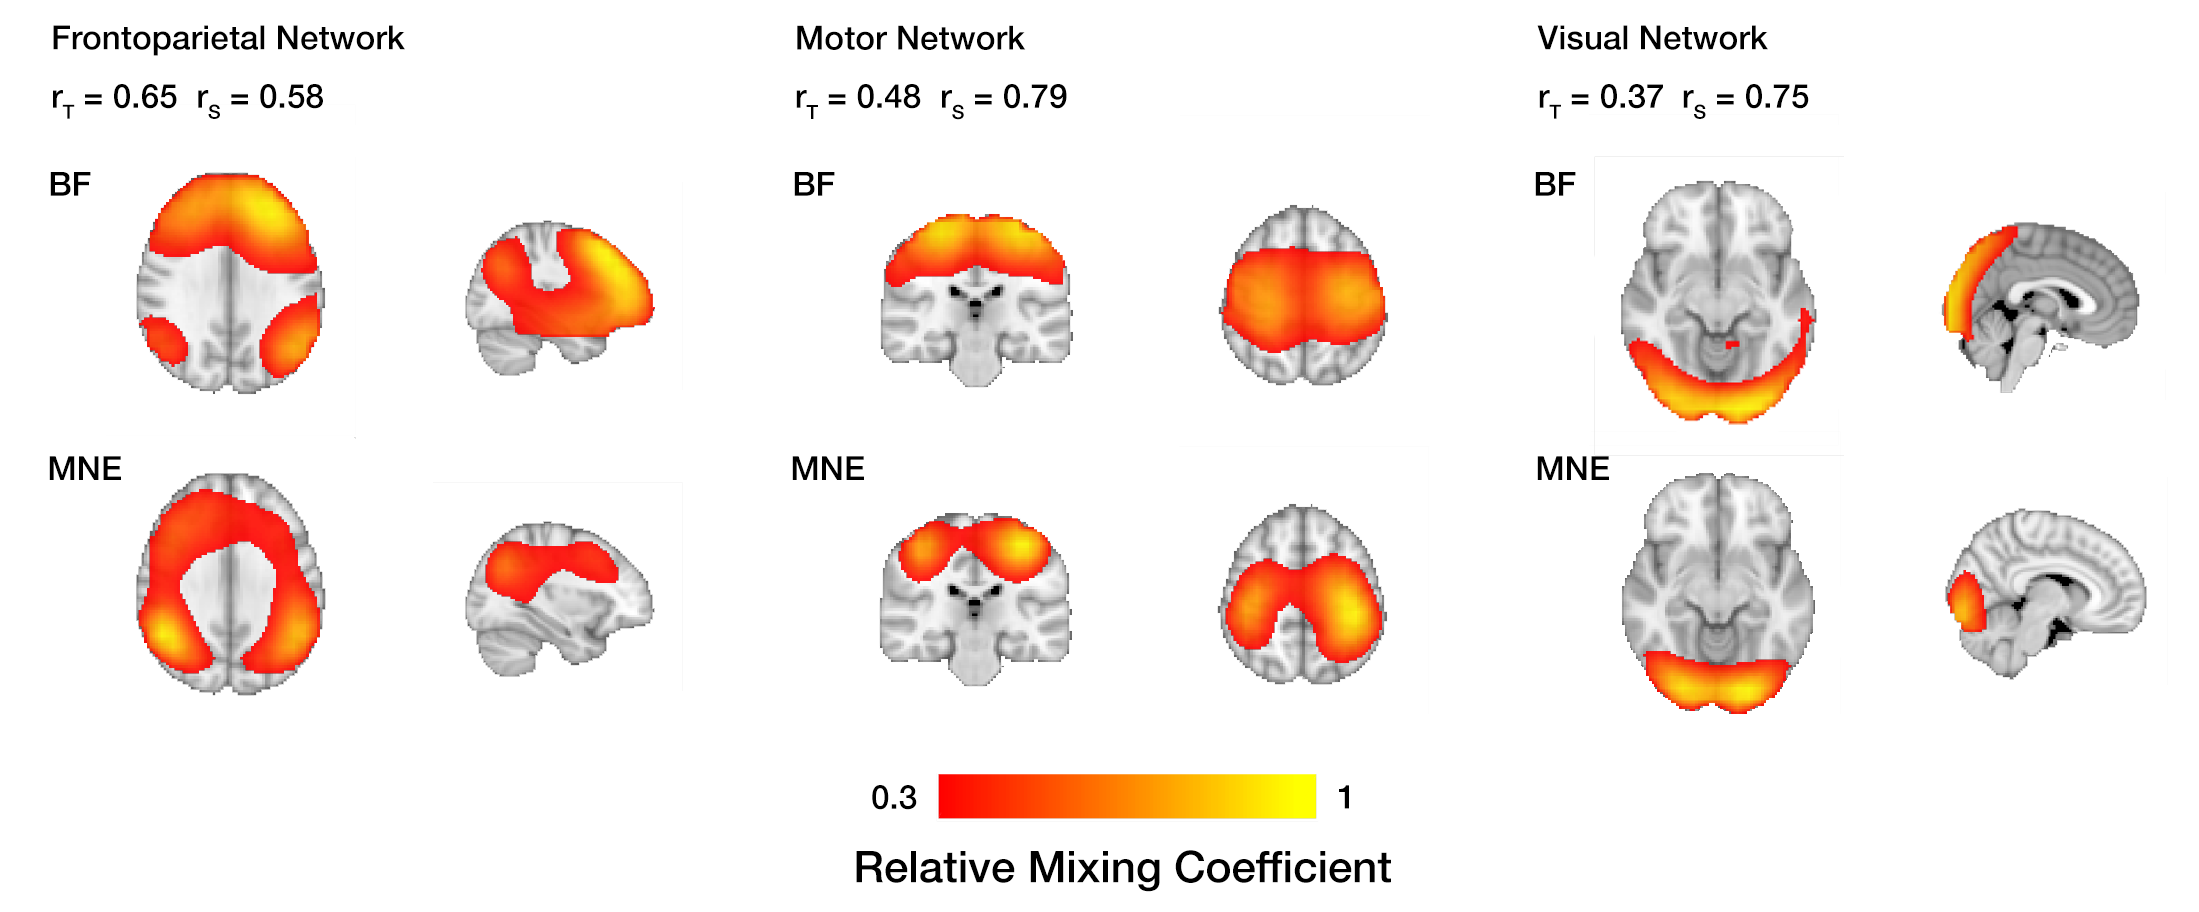
\includegraphics[width=\textwidth]{./images/chapter2/fig_03.png}
		\caption{Spatial distributions of temporally matched functional networks, derived from both beamformer and MNE reconstructed resting state MEG data. Spatial topographies of 3 networks (Visual, Motor and Fronto-Parietal) are shown, based on the columns of the mixing matrix \textbf{A} in Equation \ref{eqn_ica}. Networks were thresholded at an arbitrary level for clarity.  Note the similarity across the two inverse methods.}\label{fig_bf_mn_4}
		\end{centering}
	\end{figure}

\begin{figure}[h!]
	\begin{centering}
		\includegraphics[width=\textwidth]{./images/chapter2/Nback.png}
		\caption{Results from the N-Back study. A) Fronto-parietal Network, extracted using ICA applied to the N-Back data. B-C) The mean signal and signal variance of the IC timecourses corresponding to the fronto-parietal network. Bar charts show the case for beamformer (blue) and minimum norm (red) solutions.
			}\label{fig_bf_mn_5}
		\end{centering}
	\end{figure}
	
	\clearpage	
\subsection{Discussion}

In this investigation, we aimed to assess the effectiveness of two inverse solutions (beamformers, and minimum norm) with regards to functional connectivity mapping. The question posed in the introduction was: can both these methods, even though their underlying assumptions are fundamentally different, produce similar connectivity results in time, space, and the estimated network response to a task? Focusing first in the time domain, we selected an arbitrary threshold of $r_t > 0.3$ to define meaningful correlation between beamformer and minimum norm derived components. Using this criterion, it was found that many beamforming ICs would strongly correlate to (in most cases) just one minimum norm IC. The strongest correlation in the resting state data (top-left element in red in Figure \ref{fig_bf_mn_3}) had a correlation of  $r_t = 0.65$, this implies that both inverse methods share significant temporal characteristics when SNR is adequate. These temporal similarities appear to be robust across studies as the networks could be replicated with both solutions in the N-Back task. In addition these temporal similarities mean that the results of the N-Back study in Figure \ref{fig_bf_mn_5}B and C are similar, with both solutions showing the same isotropic decline variance in the Frontoparietal network when the task increases in difficulty. 

When assessing the spatial attributes of the two methods the similarities continue. The spatial correlations of the reconstructed electrophysiological networks are largely higher than their temporal counterparts. However this may be due to the lower dimensionality of the data in the spatial domain (which corresponds to approximately the number of sensors in a MEG system, in this case it was $\sim$275). Qualitatively, it is not difficult to see that whilst there are some notable differences in the network maps, the general topographies are similar.

Whilst there are clear similarities shown, there are some differences in the network topographies between these two solutions. As the depth scaled equations for both weights (Equations \ref{eqn_weights_dspm} and \ref{eqn_weights_z_2}) differ in only which matrix ($\mathbf{C}$ and $\mathbf{G}$) is in between the lead fields, it is imperative to understand what both are doing. $\mathbf{C}$ being data driven has been shown to make reconstruction more sensitive in areas where activity is more pronounced and less so to brain regions with low SNR \citep{VanVeen1997,Gross2001,Barnes2003}, which makes it ideal at reconstructing oscillatory sources over small regions of brain volumes by accentuating oscillations over a small spatial region. The gram matrix $\mathbf{G}$ however, is a model based upon the geometry of the brain and its position in the MEG system, which gives a similar sensitivity profile around the cortex, giving its reconstructions a 'smudged' characteristic.

That question is, given the similarity of the results, which reconstruction method do we select? Here, we have selected beamformers for a number of reasons. It could be argued that the correlated source suppression will be a hindrance when assessing functional connections, but in practice it will only happen when the correlation between sources is 0.7 or higher \citep{VanVeen1997} or highly correlated for over 40\% of the window which covariance is estimated \citep{Hadjipapas2005}; in practice this is unlikely other than in special cases (such as binaural steady state experiments) or if covariance is assessed over short windows. Secondly, whilst minimum norm is better at reconstructing large regions of evoked activity \citep{Ou2009}, we are intending to look at oscillatory power signatures at smaller spatial scales of connectivity, of which the power estimation of beamforming is better suited \citep{Jensen2010}. This is because unlike minimum norm, it does not try to localise sources based on observations, but rather estimates power at a selected ROI. Also there is the issue of the lack of interference rejection in minimum norm. Whilst you could regress out interference with ICA de-noising methods \citep{Mantini2007}, the automatic rejection of interference with beamforming is an attractive feature. Likewise, not having to make an \textit{a-priori} selection of the number of sources to model makes it particularly flexible for assessment of connectivity on multiple spatial scales; which is useful in the context of the work presented in this thesis, which operates at a single voxel level up to large volumes of brain space. As a final note the MEG laboratory here in Nottingham has gained extensive experience with beamformers over the past decade \citep{Brookes2005,Brookes2007,Brookes2008,Zumer2010,Stevenson2011,Brookes2011a} and so we are in a better position to use them.
\clearpage

\section*{Summary}

In this second theory chapter, we have explained the necessary steps to successfully localise MEG sources, which allows us to circumvent the confounds of sensor level functional connectivity analysis. In reconstructing data back into source space, we allow ourselves to gain a deeper understanding of where functional connections may occur. In the next chapter we introduce methods of functional connectivity analysis which take advantage of the spatial specificity our MEG data now possesses, and crucially the high temporal resolution to image dynamic functional connections.  
\setstretch{1.0}
\chapter{Measuring Functional Connectivity in MEG}\label{chapter_fc_and_leakage}

In this chapter, the commonly used methods to measure functional connectivity using source reconstructed data are introduced. Whilst not intended as an exhaustive review of every connectivity metric, it covers many of the technical aspects that need to be addressed for a successful study. Also in this chapter the concept of signal leakage is introduced. This arises from source reconstruction errors and, if not carefully controlled for, will confound results. We introduce a model to characterise and correct for signal leakage, allowing for a confident assessment of functional connectivity. 

\doublespacing

\section*{Introduction}
Following the projection of MEG data into source space, achieved (in the case of this thesis) with beamforming, we can now turn our attention to the main focus of this thesis, the assessment of the functional connections within the brain. To reiterate Chapter \ref{chap_intro}, functional connections are defined as a \textit{statistical interdependency} between measured activity at two (or more) spatially separate regions of the brain \citep{Friston2011}. In fMRI, the term "functional connectivity" has become synonymous with the correlation of BOLD timecourses, but for MEG, the definition is considerably broader. The rich content of MEG data allows functional connectivity to be derived in many different ways, and whilst a number of types of coupling have become prominent, two in particular stand out for their popularity. The first arises from a fixed phase relationship between band-limited oscillatory signals (i.e. phase synchronisation), the second is the result of synchronisation between the amplitude envelopes of band limited oscillations; these will be discussed in more detail throughout the chapter.

Despite the advantages of source space estimation discussed in Chapter \ref{chapter_meg_source}, a significant technical confound arises from source reconstruction, which is typically termed “signal leakage”. The ill-posed nature of the MEG inverse problem \citep{Hadamard1902} causes a degree of spatial blurring in source space reconstruction. This means that a single point source will appear to spread across a finite volume. In addition to this spread, it is also possible for sources to be mislocalised, for example due to inaccuracies in modelling the forward vector or because of deviations from the assumptions driving the inverse model. This has a profound effect on functional connectivity calculations, as it has the tendency to artefactually inflate connectivity levels between regions. 

In this chapter we discuss the techniques to measure functional connectivity without the confound of signal leakage.  Section \ref{sec_fc_1} gives a brief overview of popular methods to assess functional connectivity. Section \ref{sec_signal_leakage} introduces the problems of artefactual functional connectivity as the result of signal leakage, with the aid of an analytical model and simulations, with Section \ref{sec_signal_corr} discussing potential solutions.

\section{Functional Connectivity Methods}\label{sec_fc_1}

At its simplest, functional connectivity measures the relation between two time series; but so rich are the properties of the MEG signal, that many different tests could be considered. In a review on functional connectivity by \cite{Engel2013}, they suggest that there are two types of intrinsic coupling modes (ICMs)\footnote{Admittedly, this does over simplify the wider picture, as there are methods which look at phase-amplitude coupling \citep{Canolty2006,Florin2015} and those which asses coupling across frequencies \citep{Canolty2010,vanWijk2014}, but the two catagories mentioned in the main text are by far the most popular.}, those which assess the relation of power between two signals (Envelope coupling), and those which look at the synchrony of the data based on their phase (Phase coupling). Examples of this are illustrated in Figure \ref{figure_3_a}. 

\begin{figure}[h!]
	\begin{center}
		\includegraphics[width=0.9\linewidth]{./images/chapter3/fig_conn_1.png}\caption{Schematic diagram of phase and envelope based connectivity analyses based upon neural oscillations. A) Envelope coupling is based upon correlation between the oscillatory envelopes of two band limited sources. B) Phase coupling typically seeks to quantify the relation of the phases of two signals, in this case the two signals have a constant difference of π.}\label{figure_3_a}
	\end{center}
\end{figure}

These two categories of coupling methods, which focus on different aspects of the MEG signal, tend to reveal different parts of the wider functional connectivity picture \citep{Scholvinck2013}. Amplitude connectivity tends to better resemble the long range connections seen in fMRI and phase based measurements less so \citep{Brookes2011a,Tewarie2016}. This is possibly reflected in invasive measurements where amplitude correlations appear to be longer ranging than correlation of the raw signals \citep{Leopold2003}. However that is not to say that phase based measurements do not have their place in electrophysiological functional connectivity analysis, as they have been used successfully in many electrophysiological studies \citep{Gross2001,Nolte2004,Jerbi2007,Kujala2007,Guggisberg2008,Hillebrand2012,Marzetti2013}. Support for a multi-metric analysis (one which combines amplitude and phase connectivity assessments) has been shown in a recent study, where combination of concurrent phase and amplitude connectivity measurements better predict the connectivity patterns seen in fMRI than either amplitude or phase metrics can individually \citep{Tewarie2016}. 

In this thesis, we utilise amplitude coupling for connectivity assessment, due to the success it has had in the past to replicate results seen in fMRI in both task and resting paradigms and its robustness to low SNR-data \citep{Colclough2016}. However for the sake of completeness, we cover some of the most popular connectivity metrics which use either amplitude of phase coupling approaches. 

\subsection{Amplitude envelope coupling}\label{sec_3_hilbert}

Prior to the growth in functional connectivity analysis, there was a large body of work probing relationships between the haemodynamic response and changes in amplitude of neural oscillations. The primary finding is that good spatial correlation exists between haemodynamic and electrical oscillatory activity, across a broad range of electrophysiological frequencies. \citep{Logothetis2001,Singh2002,Moradi2003,Brookes2005,Mukamel2005,Winterer2007,Muthukumaraswamy2008,Zumer2010,Stevenson2011,Stevenson2012}. In addition, there is a general trend for a negative relationship between BOLD and low (alpha and beta) frequency oscillations (i.e. when alpha and beta oscillations decrease in power, the BOLD response typically increases) and a concomitant positive correlation between BOLD and high frequency (gamma band) oscillations \citep{Hall2014}. There are many methods which can be used to look at the relations between oscillatory power, but arguably the simplest is to assess their correlation. 

To asses the relationship of fluctuating power between two signals, we need to first create their amplitude envelopes. There are many methods to generate the amplitude envelope of the signal, ranging from continuous (Morlet) transform \citep{Quyen2001,Kiebel2005} to the S-transform \citep{Stockwell1996}, however the most popular is the Hilbert transform which has been extensively covered in the literature \citep{Tass1998,Quyen2001,Freeman2004,Kiebel2005}. Assuming a source reconstructed timecourse $\hat{q}(t)$, then its complex 'analytical signal' is given by

\begin{equation}
\hat{z}(t)=\hat{q}(t)+iH\big[\hat{q}(t)\big]
\end{equation} where \textit{H} is the Hilbert transform which is the convolution of the function $\frac{1}{\pi t}$ with $\hat{q}(u)$,

\begin{equation}
H\big[\hat{q}(t)\big]=P\Bigg[\frac{1}{\pi}\int_{-\infty}^{\infty}\frac{\hat{q}(u)}{t-u}\text{d}u\Bigg]
\end{equation} where \textit{P} is the Cauchy principal value of the integral, which is necessary to account for the singularity which occurs when $t=u$. The signal envelope is then given by

\begin{equation}
E\big[\hat{q}(t)\big] = \sqrt{\big(\hat{q}(t)\big)^2+\big(H\big[\hat{q}(t)\big]\big)^2}\label{eqn_3_19}
\end{equation} Note that $E\big[\hat{q}(t)\big]$, is a non-linear and non-reversible transform of $\hat{q}(t)$. The instantaneous phase data contained within $\hat{q}(t)$, which can be obtained directly from the Hilbert transform as

\begin{equation}
\phi(t)=\text{atan}\Bigg(\frac{H[\hat{q}(t)]}{\hat{q}(t)}\Bigg), \label{eqn_3_hilbert_phase}
\end{equation} is discarded by Equation \ref{eqn_3_19} and is not used on envelope based connectivity metrics. Following envelope calculation, correlation can be calculated simply: if $\mathbf{X}$ is a $1 \times P$ vector representing the envelope of the seed source, and $\mathbf{Y}$ is a $1 \times P$ vector representing the envelope of the leakage corrected test source, connectivity can be estimated as

\begin{equation}
r(\mathbf{X},\mathbf{Y}) = \frac{\mathbf{XY}^T}{\sqrt{\mathbf{XX}^T}\sqrt{\mathbf{YY}^T}}\label{eqn_3_20}
\end{equation} where \textbf{X} and \textbf{Y} must have been mean corrected prior to testing. Note that Equation \ref{eqn_3_20} simply represents a pearson correlation coefficient. Keeping the seed static and test moving around the brain enables high resolution maps of connectivity between the seed and the rest of the brain volume. But this is unable to show directly how other regions are connected at the same time without performing an exhaustive search of every possible voxel pair in the brain. However, as we are determining the linear relationship between amplitude envelope signals, it is possible to reformulate Equation \ref{eqn_3_20} in the context of linear regression \citep{Hall2013}. Here the test envelope \textbf{Y} is explained by a general linear model (GLM), where \textbf{X} is used to form the design matrix, $\beta$ represents the regression parameter and $\mathbf{\Delta}$ the error.

\begin{equation}
\mathbf{Y} = \beta\mathbf{X} + \mathbf{\Delta}, \label{eqn_3_21}
\end{equation} the regressive parameter can be estimated with $\beta=\textbf{X}^+\textbf{Y}$, where the superscript + denotes the pseudoinverse. It has been shown , for the case where the design matrix is a single column, that $r(\mathbf{X},\mathbf{Y}) \propto \beta$ \citep{Hall2013}. The beauty of the GLM framework in Equation \ref{eqn_3_21} is that the design matrix can be extended to incorporate more columns, which allows for the test to be expanded into a multivariate test (c.f Chapter \ref{chapter_cca}). An advantage of this multivariate framework is that we can include signals of no interest (from larger clusters of data) without it confounding the connectivity estimation.

\subsection{Phase based measurements}
Multiple metrics are available to assess functional connectivity in raw projected data and these are reviewed briefly here.

\subsubsection{Coherence}
One of the most popular phase based metrics is to measure the coherence of two signals. Coherence provides information about the level of coupling between two signals at a specific frequency component, and can be thought of as correlation in the Fourier domain. If we have two signals $x(t)$ and $y(t)$, then their coherence $M_{xy}$ can be calculated as

\begin{equation}
M_{xy}(f) = \frac{\big|C_{xy}(f)\big|^2}{C_{xx}(f)C_{yy}(f)},
\end{equation} where $C_{xy}$ is the cross-spectral density between the two signals, which is measured from the Fourier transformed signals $X(f)$ and $Y(f)$. 

\begin{equation}
C_{xy}(f) = X(f)Y^*(f),
\end{equation} where the superscript $*$ represents the conjugate transpose of an array. Coherence values range from $0 \leq M_{xy} \leq 1$ with 1 representing perfect coupling. Coherence has been widely used for measuring connectivity in MEG, largely in part to the success of dynamic imaging of coherent sources (DICS; \citealp{Gross2001}) method which uses a frequency domain beamformer to localise sources coherent with a reference signal. Coherence has been shown to be particularly useful between cortical sources in MEG and EMG hand movement experiments \citep{Gross2001}, but also between regions during tasks \citep{Kujala2007,Bardouille2012}.

\subsubsection{Phase locking}
It has been argued that coherence is not a true measurement of the phase relationship between two signals \citep{Lachaux1999}, this is because coherence results can be affected by modulations in amplitude, or covariance between the two signals, especially when the SNR of the signals are low. The alternative is to use a measure that specifically identifies when transient phase locking has occured, which is precisely what the phase locking value (PLV; \citealp{Lachaux1999}) sets out to achieve. Starting with two signals $ x(t) $ and $ y(t) $, they are band-pass filtered to a band of interest and the instantaneous phase of each signal, defined as $ \phi_x(t) $ and $ \phi_y(t) $ respectively. Typically the instantaneous phase is acquired from a Wavelet or Stockwell transform, but the Hilbert transform (in particular Equation \ref{eqn_3_hilbert_phase}) would be equally valid as a method to extract instantaneous phase. We then compute the phase difference between the two signals at each time point $\theta(t) = \phi_x(t) - \phi_y(t)$. The phase locking value (PLV) is then given by

\begin{equation}
\text{PLV} = \frac{1}{T}\sum_{t}^{T}\text{e}^{i\theta(t)},
\end{equation} where \textit{T} is the number of time samples in the signal. We can also look for consistent phase difference over repeats of a stimulus in multi-trial data at the same time point, \textit{t}, within a trial

\begin{equation}
\text{PLV}(t) = \frac{1}{N}\sum_{n}^{N}\text{e}^{i\theta(t,n)},
\end{equation} where \textit{n} is the trial index and \textit{N} is the total number of trials. A graphical description of this can be found in Figure \ref{fig_phase}A.

\subsubsection{Phase metrics and leakage}
Both coherence and PLV are sensitive to source leakage and so modified algorithms have been introduced to protect them from the contamination of such artefacts. For coherence this is done by merely assessing the imaginary component of the cross spectral density, which tends to zero if the phase difference is close to 0 or π \citep{Nolte2004} such that

\begin{equation}
M_{xy}(f) = \frac{\big|\text{Im}\big(C_{xy}(f)\big)\big|^2}{C_{xx}(f)C_{yy}(f)}.
\end{equation} To make PLV measures invariant to leakage the Phase Lag Index (PLI; \citealp{Stam2007}) was introduced. The PLI suggests that the distribution of $\mathbf{\theta}$ across all time will be symmetric if there is no genuine connections or if $ \mathbf{\theta} $ is centred around 0 or $\pm$π. Conversely if there is genuine phase locked connectivity then the distribution will be skewed. The PLI measures the skew using

\begin{equation}
\text{PLI} = \Bigg|\frac{1}{T}\sum_{t}^{T}\text{sign}\Big(\text{Im}\big(\text{e}^{i\theta(t)}\big)\Big)\Bigg|,
\end{equation} where $\text{sign}(\theta)=1$ for a positive value and -1 for a negative value and 0 for null terms. Again, like imaginary coherence, by taking just the imaginary part of the exponential, π-phase relations are nullified and so have no contribution to the summation in Equation 4.12, (as seen in Figure \ref{fig_phase}B). PLI has values ranging from 0 (symmetric distribution; no connectivity other than possibly leakage) to 1 (strongly connected).


\begin{figure}
	\begin{center}
		\includegraphics[width=\linewidth]{./images/chapter3/phase.png}\caption{Graphical descrptions of the phase coupling methods. Panel A shows the Phase Locking Value (PLV; \citealp{Lachaux1999}). On the Argrand diagram, the phase lags from a region of interest are represented by the blue arrows. The red arrow represents the PLV result. Note that the point which represents leakage at -π contributes to the final result. Panel B represents the Phase Lag Index (PLI; \citealp{Stam2007}). The same 6 phase lags have now been converted with the sign function, with the lag representing leakage now nullified (represented as the blue $\times$ at 0) so no longer contributes.}\label{fig_phase}
	\end{center}
\end{figure}

\section{Characterising signal leakage}\label{sec_signal_leakage}
\subsection{Analytic model}
In order to better understand the leakage effect, a simple analysis proves helpful. Consider the case of two sources: $\mathbf{q}_1$, which is of dimension $1 \times P$ and represents the timecourse at location $\mathbf{r}_1$. $\mathbf{q}_2$ shares the same dimensions and represents the timecourse at location $\mathbf{r}_2$. $P$ denotes the number of temporal samples in the data. $\mathbf{q}_1$ and $\mathbf{q}_2$ are assumed to be orthogonal, such that the covariance $\tfrac{1}{P}\mathbf{q}_1\mathbf{q}_2^T = 0$. Recalling the generative model in Section \ref{sec_gen_model}, if there are no other sources in the brain, then the $N \times P$ MEG data matrix can be described as:

\begin{equation}
\mathbf{m} = \mathbf{l}_1\mathbf{q}_1+\mathbf{l}_2\mathbf{q}_2 + \mathbf{e}, \label{eqn_leak_model_1}
\end{equation} where $\mathbf{l}_1$ and $\mathbf{l}_2$ (both of dimension $N \times 1$) are the forward solutions for sources $\mathbf{q}_1$ and $\mathbf{q}_2$ respectively. $\mathbf{e}$ shares the same dimensions as $\mathbf{m}$ and represents sensor noise. Using a source localisation technique (such as beamforming) to reconstruct $\mathbf{q}_1$:

\begin{equation}
\hat{\mathbf{q}}_1 = \mathbf{w}_1^T\mathbf{m} \label{eqn_leak_model_2}
\end{equation} where $\mathbf{w}_1$ represents the weights vector for location $\mathbf{r}_1$. Substituting Equation \ref{eqn_leak_model_2} into \ref{eqn_leak_model_1} and using the linear constraint for beamformer weights that $\mathbf{w}^T\mathbf{l} = 1$ the reconstructed source $\hat{\mathbf{q}}_1$ can be represented as

\begin{equation}
	\begin{aligned}
	\hat{\mathbf{q}}_1 &= \mathbf{w}_1\mathbf{l}_1\mathbf{q}_1 + \mathbf{w}_1^T\mathbf{l}_2\mathbf{q}_2 \\
	&= \mathbf{q}_1 + \mathbf{w}_1^T\mathbf{l}_2\mathbf{q}_2.
	\end{aligned}\label{eqn_leak_model_3}
\end{equation} What this means is that the beamformer reconstruction for source 1 is only independent of source 2 if $\mathbf{w}^T_1\,\mathbf{l}_2=0$. Similarly, reconstructing source 2 gives

\begin{equation}
\hat{\mathbf{q}}_2 = \mathbf{q}_2 + \mathbf{w}_2^T\mathbf{l}_1\mathbf{q}_1.\label{eqn_leak_model_4}
\end{equation} Given that the two sources are independent, it follows that the source leakage, $s$, can be generated by calculation of the covariance between the two reconstructed timecourses (i.e $s=\tfrac{1}{P}\hat{\mathbf{q}}_1\hat{\mathbf{q}}_2^T$). Substitution of Equations \ref{eqn_leak_model_3} and \ref{eqn_leak_model_4} gives

\begin{equation}
\begin{aligned}
s &= \tfrac{1}{P}\hat{\mathbf{q}}_1\hat{\mathbf{q}}_2^T \\
&= \tfrac{1}{P}\Big(\mathbf{q}_1 + \mathbf{w}_1^T\mathbf{l}_2\mathbf{q}_2\Big)\Big(\mathbf{q}_2 + \mathbf{w}_2^T\mathbf{l}_1\mathbf{q}_1\Big)^T\\
&= \tfrac{1}{P}\Big(\underbrace{\mathbf{q}_1\mathbf{q}_2^T}_\text{=0}+\mathbf{q}_1\mathbf{w}_2\mathbf{l}_1^T\mathbf{q}_1^T+\mathbf{q}_2^T\mathbf{w}_1^T\mathbf{l}_2\mathbf{q}_2+\underbrace{\mathbf{w}_1^T\mathbf{l}_2\mathbf{q}_2\mathbf{w}_2\mathbf{l}_1^T\mathbf{q}_1^T}_{=0}\Big) \\
&=\mathbf{w}_2^T\mathbf{l}_1\nu_1+\mathbf{w}_1^T\mathbf{l}_2\nu_2,
\end{aligned}\label{eqn_leak_model_5}
\end{equation} where $\nu_1=\tfrac{1}{P}\mathbf{q}_1\mathbf{q}_1^T$ and $\nu_2=\tfrac{1}{P}\mathbf{q}_2\mathbf{q}_2^T$. What this model shows is that the leakage term will only drop to zero if the weights of one source are orthogonal to the forward solution to the other source and vice versa. It should be noted that this model assumes zero noise (i.e the noise term from Equation \ref{eqn_leak_model_1} has been ignored), however in practice the addition of sensor noise will lower the covariance between sources (and therefore the leakage) so Equation \ref{eqn_leak_model_5} represents and upper limit on leakage between two sources.

\subsection{Simulations}
It proves instructive to extend this model in simulation. The simulations were based on a two source model equivalent to that described above. In all cases a seed source ($\mathbf{q}_2$) was placed approximately in the right primary sensorimotor cortex. 2781 iterations of the simulation were run, and on each iteration the test source ($\mathbf{q}_1$) was simulated in a different voxel. Voxels were placed on an 8 mm cubic grid spanning the entirety of brain space. Dipole orientation was allowed to vary smoothly with position in order to mimic dipole orientations in real MEG data. The source magnitudes were 8 nAm and source timecourses were generated from a beamformer reconstruction of a resting state MEG experiment. Source timecourses were phase randomised (\citealp{Prichard1994}; see Section \ref{phase_randomisation} for a mathematical description) so as to have zero (or as little as possible) correlation between them. The geometry for the simulation were based on the CTF MEG system in Nottingham operating in third order synthetic gradiometer configuration. The location of the MEG sensors with respect to brain anatomy was based on a real experimental recording session. Two separate noise models were used, in case 1, sensor noise was drawn from a Gaussian random process (meaning noise was uncorrelated across sensors). In case 2, real MEG noise was employed (where interference is correlated across MEG sensors). This was generated via the recording of 300 s of real MEG data with no subject in the system. 

The results of this simulation are shown in Figure \ref{figure_3_1}. Figure \ref{figure_3_1}A shows images of the magnitude of leakage between the seed source, and test sources at all other locations in the brain. The top two rows shows shows Gaussian sensor noise whereas the bottom rows shows realistic noise. The group of 4 images shows the analytical case (which reflects an upper limit on leakage based on Equation \ref{eqn_leak_model_5}) the results from the actual simulation. Note that in all cases source leakage is at its worst in brain areas adjacent to the seed. Note also that leakage worsens when using a realistic noise model. Figure \ref{figure_3_1}B shows equivalent leakage images for shallow (left) and deep (right) grey matter sources. It is clear that source leakage worsens for deeper sources due to their lower signal to noise ratio. Finally in Figure \ref{figure_3_1}C the upper panel shows the relationship between the analytical model in Equation \ref{eqn_leak_model_5}, and the actual simulation where the analytical model gives an upper limit on leakage. The lower panel of Figure \ref{figure_3_1}C shows leakage magnitude as a function of Euclidian distance between the seed and test voxels. Note that even sources separated by as much as 5 cm can exhibit a large amount of signal leakage, which would significantly confound any attempt at functional connectivity analysis. As shown by the above simulation, signal leakage differs depending on the brain area being studied, the signal to noise ratio of the data and the sensor level noise model. In addition, it depends on the inverse solution being used \citep{Scoffelen2009}, and the number of dipoles active in the brain. As can be seen from the images in Figure \ref{figure_3_1}A, the spatial profile of leakage is asymmetric around the seed location.

\begin{figure}[h!]
	\begin{center}
		\includegraphics[width=\linewidth]{./images/chapter3/Figure_1.png}\caption{Examples of source space signal leakage. A) Images showing the magnitude of leakage between a simulated source in the primary sensorimotor cortex (blue dot), and equivalent simulated sources placed at all other brain locations. The upper panels show the analytical worst-case scenario whereas the lower panels show results from the actual simulation. The upper panels shows simulated Gaussian sensor level noise (i.e. the noise is uncorrelated across channels) whereas the lower panels shows realistic noise (which is correlated across the channels). Note in all cases that source leakage is worst close to the seed and typically spreads asymmetrically around the seed. Note also that leakage worsens with a realistic noise model. B) Equivalent images for a shallow cortical source (left) and a deep source (right); leakage worsens for deeper sources which exhibit a lower signal to noise ratio. C) Upper panel shows the relation between the analytical model in Equation 9, and the actual simulation for every test voxel; note the analytical model gives a “worst case scenario” regarding the leakage, which is reduced in the simulation via the addition of sensor level noise. The lower panel shows leakage magnitude as a function of Euclidian distance between the seed and the test voxels.\label{figure_3_1}}
	\end{center}
\end{figure}
\clearpage

\section{Correcting for signal leakage}\label{sec_signal_corr}
A number of potential solutions to the source leakage problem have been proposed \citep{Nolte2004,Stam2007,Brookes2012b,Hipp2012,Ewald2012,Marzetti2013,Brookes2014,ONeill2015A,Colclough2015,Wens2015} Although separate methods have different modes of operation, they are all based on the observation that leakage generates altered connectivity between estimated sources, which manifests as a zero-phase-lag correlation. Indeed this is shown by Equations \ref{eqn_leak_model_3} and \ref{eqn_leak_model_4}, which imply that leakage results in a weighted addition of a distal source. Genuine connectivity, on the other hand, is more likely to incorporate a time lag, generated as electrical signals travel between different brain regions. This means that elimination of all zero-phase-lag correlations in source space should result in the elimination of leakage, albeit at the expense of a loss of genuine zero-phase-lag connectivity (which has been shown to exist in invasive recordings; \citealp{Singer1999}). The application of beamforming supresses temporally correlated sources and this potentially aids leakage reduction. However for such suppression to occur, sources must be highly correlated ($r > \sim 0.7$ – which is unlikely for anything other than driven steady state responses) and therefore even after beamforming, further steps must be taken if leakage artefacts are to be controlled. In phase based connectivity metrics, leakage reduction methods usually circumvent zero-phase (and conversely π-phase) connections by assessing only the imaginary part of a signal in the Fourier domain \citep{Nolte2004,Nolte2008,Ewald2012,Marzetti2013} or by focusing on the asymmetry of the phase difference distribution \citep{Stam2007,Vinck2011}. In the case of metrics which employ amplitude data, methods have been derived to regress out the zero-phase relationship at source level, prior to connectivity analysis.

\subsection{Pairwise regression}
Consider again two beamformer estimated timecourses $\hat{\mathbf{q}}_1$ and $\hat{\mathbf{q}}_2$ representative of two underlying sources with a linear zero-phase-lag relationship caused by leakage. To mitigate the leakage, a linear projection of the seed voxel, $\hat{\mathbf{q}}_2$, is removed from the test voxel $\hat{\mathbf{q}}_1$. Mathematically, a general linear model is applied such that

\begin{equation}
\hat{\mathbf{q}}_1 = \beta\hat{\mathbf{q}}_2 + \hat{\mathbf{q}}_{1M}
\end{equation} where $\beta$ represents the effect size and relates directly to the magnitude of the leakage. $\hat{\mathbf{q}}_{1M}$ is the residual measurement, which represents the leakage-suppressed timecourse for the test location (i.e $\hat{\mathbf{q}}_{1M}$ is the beamformer estimate of activity in $\hat{\mathbf{q}}_1$, but with the linear dependence on $\hat{\mathbf{q}}_{2}$ [leakage] removed). $\beta$ can be estimated as.

\begin{equation}
\beta = \hat{\mathbf{q}}_1\hat{\mathbf{q}}_2^+ \label{eqn_3_7}
\end{equation} where the superscript $+$ denotes the Moore-Penrose pseudo-inverse. 

Figure \ref{figure_3_2} shows an example of envelope based functional connectivity taken from a real MEG recording in a single subject. Five minutes of MEG data were recorded using the CTF MEG system in Nottingham (note: these data were first presented in a study by \cite{Brookes2011a}). The subject was asked to lie in the system and “think of nothing” whilst connectivity was assessed, over all time, between a seed location in left sensorimotor cortex and all other voxel locations in the brain. In the upper panel, connectivity was computed between the seed and all other test voxels with no leakage reduction applied. In the lower panel, leakage reduction has been employed using the method outlined above. In both cases, envelopes of beta band (13-30 Hz) oscillations were employed. It is clear that a functional network of brain regions exists in the data, with the beta band envelope in left motor cortex showing high levels of correlation with equivalent envelopes in homologous regions of right sensorimotor cortex. In addition, note the significant advantages afforded by the reduction in zero-phase-lag correlation. In the uncorrected case, regions showing high connectivity extend from the seed voxel towards the centre of the brain as well as into the left temporal lobe. The spatial profile of leakage is in good agreement with the simulation presented in Figure \ref{figure_3_1}. This blurring around the seed location is reduced when applying leakage reduction.  

\clearpage

\begin{figure}[h!]
	\begin{center}
		\includegraphics[width=\linewidth]{./images/chapter3/Figure_2.png}\caption{An illustration of leakage correction. Top Panel: Envelope correlation in real data between a seed in right motor cortex and all other brain locations, prior to reduction of leakage. Bottom Panel: Envelope correlation for the same data, post leakage reduction.\label{figure_3_2}}
	\end{center}
\end{figure}


\subsection{Limitations and signal kurtosis}

Despite the advantages of leakage reduction strategies, they have significant limitations, which should be discussed. Firstly, the pairwise method does not make the modified test timecourse, $\hat{\mathbf{q}}_{1M}$, a faithful reconstruction of the true source timecourse $\hat{\mathbf{q}}_1$. In fact, the modified timecourse retains an element of leakage from $\hat{\mathbf{q}}_2$. Only the magnitude of that leakage is altered, in such a way as to ensure orthogonality between $\hat{\mathbf{q}}_{1M}$ and $\hat{\mathbf{q}}_2$. To demonstrate this recall Equations \ref{eqn_leak_model_3} and \ref{eqn_leak_model_4}, the reconstructed sources $\hat{\mathbf{q}}_1$ and $\hat{\mathbf{q}}_2$ are defined as

\begin{equation}
\begin{aligned}
\hat{\mathbf{q}}_1 &=\mathbf{q}_1 +a\mathbf{q}_2 \\
\hat{\mathbf{q}}_2 &=\mathbf{q}_2 +b\mathbf{q}_1
\end{aligned}
\end{equation} where $a = \mathbf{w}^T_1\mathbf{l}_2$ represents the leakage from the seed source $\mathbf{q}_2$ to the test $\mathbf{q}_1$ and $b = \mathbf{w}^T_2\mathbf{l}_1$ is the leakage in the opposite direction. Using the leakage reduction algorithm described above the leakage estimate, $\beta$ is given by a Moore Penrose pseudoinverse, thus:

\begin{equation}
\begin{aligned}
\beta &= \big[\hat{\mathbf{q}}_2^T\hat{\mathbf{q}}_2\big]^{-1}\hat{\mathbf{q}}_2^T\hat{\mathbf{q}}_1\\
&=\big[(\mathbf{q}_2+b\mathbf{q}_1)^T(\mathbf{q}_2+b\mathbf{q}_1)\big]^{-1}(\mathbf{q}_2+b\mathbf{q}_1)^T(\mathbf{q}_1+a\mathbf{q}_2).
\end{aligned}
\end{equation} If $\mathbf{q}_1$ and $\mathbf{q}_2$ are temporally uncorrelated such that $\mathbf{q}_1^T\mathbf{q}_2 = \mathbf{q}_2^T\mathbf{q}_1 = 0$ , then:

\begin{equation}
\begin{aligned}
\beta &= \big[\mathbf{q}_2^T\mathbf{q}_2+b^2\mathbf{q}_1^T\mathbf{q}_1\big]^{-1}(a\mathbf{q}_2^T\mathbf{q}_2+b\mathbf{q}_1^T\mathbf{q}_1)\\
&=\frac{a\sigma_2+b\sigma_1}{\sigma_2+b^2\sigma_1}
\end{aligned}
\end{equation} where $\mathbf{q}_1^T\mathbf{q}_1 = \sigma_1$ and likewise $\mathbf{q}_2^T\mathbf{q}_2 = \sigma_2$. Having found $\beta$, it becomes possible to derive an equation for the modified estimated source timecourse ($\hat{\mathbf{q}}_{1M}$) following leakage reduction:

\begin{equation}
\begin{aligned}
\hat{\mathbf{q}}_{1M} &= \hat{\mathbf{q}}_{1} - \beta\hat{\mathbf{q}}_{2}\\
&= (\mathbf{q}_{1} + a\mathbf{q}_{2})-\Bigg[\frac{a\sigma_2+b\sigma_1}{\sigma_2+b^2\sigma_1}\Bigg](\mathbf{q}_{2} + b\mathbf{q}_{1}).
\end{aligned}
\label{eqn_dyn_leak_0}
\end{equation}Which simplifies to

\begin{equation}
\hat{\mathbf{q}}_{1M} = k(\sigma_2\mathbf{q}_1 - b\sigma_1\mathbf{q}_2),
\end{equation} where $k = \frac{1-ab}{\sigma_2+b^2\sigma_1}$ is a constant. This shows that leakage reduction applied in this way does not mean that $\hat{\mathbf{q}}_{1M}$ is a corrected and hence faithful reconstruction of $\mathbf{q}_1$. Rather, it ensures $\hat{\mathbf{q}}_{1M}$ and $\hat{\mathbf{q}}_{2}$ are orthogonal. Second, as noted earlier, the method also means the removal of true zero-phase connections; this is important, particularly given that invasive recordings show significant genuine zero-phase-lag effects in the brain (Singer, 1999). 

Finally, for the regression method to work, the data need to be Gaussian distributed. This is highlighted in Figure 5B which shows results from a simple simulation. Two signals, $\mathbf{X}$ and $\mathbf{Y}$, were generated as linear mixtures of independent timecourses, $\mathbf{S}_1$ and $\mathbf{S}_2$. The first mixture was defined as $\mathbf{X}=\mathbf{S}_1-k\mathbf{S}_2$ and the second as $\mathbf{Y}=\mathbf{S}_2+k\mathbf{S}_1$. The parameter $k$ is a positive constant and controls the degree of leakage in the simulation; this was set to 0.2. Three separate simulations were undertaken in which $\mathbf{S}_1$ and $\mathbf{S}_2$ were drawn from a) Gaussian distributed noise b) leptokurtic noise (Gaussian\textsuperscript{3}) and c) uniformly distributed platykurtic noise. Leakage reduction was applied to \textbf{Y} and the result should be zero correlation between timecourses following correction. A phase randomisation approach \citep{Prichard1994} was employed to test the significance of any non-zero correlation observed and the false positive count was calculated as the number of significant measures of correlation observed across 1000 iterations of the simulation. Results show clearly that if the underlying processes ($\mathbf{S}_1$ and $\mathbf{S}_2$) are normally distributed, the false positive rate (FPR) follows the expected trend (black line). However, if $\mathbf{S}_1$ and $\mathbf{S}_2$ are either leptokurtic or platykurtic, leakage is poorly accounted for. Overall, the Gaussian assumption is reasonable; indeed it is an assumption at the heart of many of the source localisation methodologies employed in MEG. However situations exist where this is not the case, for example epileptic seizures \citep{Prendergast2013} and for this reason care should be taken when deploying the regression method to correct for leakage.

However it should be noted that considering the extensive coverage of orthogonalisations shortcomings, it is a powerful tool which vastly improves our estimates of functional connectivity analysis, and should be utilised in all MEG connectivity analyses.  

\begin{figure}[h!]
	\begin{center}
		\includegraphics[width=\linewidth]{./images/chapter3/kurtosis.png}\caption{Results of a simulation characterising the effectiveness of linear
			regression as a technique for leakage reduction. Left: The statistical distributions used
			to generate the underlying independent timecourses \textbf{S}1 and \textbf{S}2. Right: The false positives
			detected and compared to the theoretical values. Note that only underlying Gaussian
			distributed data result in agreement between the calculated and theoretical false positive
			rates and the other distributions return false positives over 96\% of the time. \label{figure_3_kurt}}
	\end{center}
\end{figure}

\clearpage
\subsection{Symmetric orthogonalisation}\label{sec_symm_orth}
In a connectivity analysis where we want to compare \textit{n} timecourses to each other to assess $n^2$ connections simultaneously (such as in Chapter \ref{chap_atlas}), pairwise orthogonalisation is not the ideal candidate to correct across all pairs simultaneously. It could be suggested that we could orthogonalise sequentially between pairs, however it poses the question of how to best approach this. In a simple case where orthogonalisation is performed between an ROI and a random (currently uncorrected) ROI, then there are (in this case) \textit{n}! possible combinations, which at $n=58$ becomes a number which is approximately the total atoms in the observable universe. Also it is not a symmetric correction to the data; that is to say the correction of source 1 based on source 2 is not equal to correcting in the opposite direction, this is shown in Figure \ref{figure_3_2a}B, where in a simple 2-dimensional case it can be clearly seen. This again could potentially prove to be a hindrance if we are assessing connections between multiple ROIs, as we have to ensure no ROI timecourses share a zero-phase relationship with any other. An elegant solution was  proposed recently by \cite{Colclough2015}, which attempts to symmetrically orthogonalise all timecourses. This method, based upon Lödwdin's symmetric orthogonalisation \citep{Lowdin1950,Mayer2002} is able to reduce linear relations between multiple separate timecourses in one calculation. The proof for this can be found in one of the aforementioned references but a description of the algorithm follows. Assume you have a measurement matrix \textbf{M}, comprising an $n \times s$ array where \textit{n} is the number of timecourses you wish to orthogonalise and \textit{s} is the number of temporal samples in each timecourse. A singular value decomposition of \textbf{M} yields

\begin{equation}
\mathbf{M}=\mathbf{USV}^T,
\end{equation} where the columns of \textbf{U} are the eigenvectors of $\mathbf{MM}^T$, the columns of \textbf{V} are the eigenvectors of $\mathbf{M}^T\mathbf{M}$ and the diagonal elements of \textbf{S} are the square root of the corresponding eigenvalues shared between \textbf{U} and \textbf{V}. To symmetrically orthogonalise all timecourses, we simply perform the calculation.

\begin{equation}
\mathbf{M}_O = \mathbf{UV}^T
\end{equation} The effect of symmetric orthogonalisation can be seen Figure \ref{figure_3_2a}C, where rather than one timecourse being adjusted like in Figure \ref{figure_3_2a}B, both are modified by the same amount. Although this might be considered a more ‘aggressive’ procedure (i.e. the resulting timecourses may be further from the original beamformed data than might be the case for pairwise correction), this technique
should be considered the method of choice for inter-regional all-to-all metrics of functional
connectivity. However it should be noted that for symmetric orthogonalisation to be correctly implemented, the number of timecourses being orthogonalised must be lower or equal to the rank of \textbf{M}; in the case of MEG data from Nottingham this corresponds to approximately the number of sensors which were used to beamform the data. This means it cannot be used in situations such as placing a seed in a voxel and investigating its connectivity to the rest of the brain volume, where the connections vastly outnumber the data rank. However in that situation as we are only interested in the influence of one voxel timecourse on the rest of the brain a pairwise correction is sufficient. 

\begin{figure}[h!]
	\begin{center}
		\includegraphics[width=\linewidth]{./images/chapter3/orthogonal.pdf}\caption{A diagram to show the effect of different leakage reduction algorithms on a two vector system. A) The two vectors showing a linear relationship. B) The effect of using the pairwise corrections methods \citep{Brookes2012b}, showing the two differing results depending on the selection of the seed \textbf{s} and test \textbf{t} vectors. C) The result of the symmetric orthogonalisation \citep{Colclough2015}, note that both vectors are modified by the same magnitude.\label{figure_3_2a}}
	\end{center}
\end{figure}

\section*{Summary}
In this chapter we have discussed the many technical facets of measuring functional connectivity in MEG. First, we introduced the measures of functional connectivity which allow us to quantify the strength of a relationship between two or more distal regions and showed that there are many approaches which a study can use before explaining that we shall use amplitude envelope coupling as our metric of choice for connectivity. Second we established that the ill posed nature of the MEG inverse problem can potentially confound results by artefactually inflating connectivity levels, and identified methods which can be used to reduce the effect this has. With all of this considered we can now proceed onto the experimental side of this thesis.

\setstretch{1.0}
\chapter{5-Dimensional dynamic connectivity}\label{chapter_cca}

Increasing evidence suggests that functional connectivity is non-stationary in time. Further, electrophysiological measurements show that connectivity is dependent on the frequency band of neural oscillations. It is also conceivable that networks exhibit a degree of spatial non-stationarity, i.e. the large scale networks that we observe may result from the time average of multiple transiently synchronised sub-networks, each with their own spatial signature. This means that the next generation of neuroimaging tools to compute functional connectivity must account for spatial, spectral and temporal non-stationarity. Here, we present a means to achieve this 5-dimensional picture via application of windowed canonical correlation analysis (CCA) to source space projected MEG data. We describe generation of time-frequency connectivity plots, showing the temporal and spectral distribution of coupling between brain regions. Moreover, CCA applied across voxels provides a means to assess spatial non-uniformity within short time-frequency windows. The feasibility of this technique is demonstrated in simulation and in a resting state MEG experiment in a single subject where we elucidate multiple distinct 5-dimensional modes of covariation between the left and right sensorimotor areas.

\doublespacing
\section*{Introduction}
So far in this thesis we have discussed multiple technical challenges associated with measuring functional connectivity using non-invasive electrophysiological data. We have discussed methods to reconstruct data in source space, allowing us to infer the spatial origin of neural signals. We then highlighted that these reconstruction methods, due to the ill-posed nature of the problem they are trying to solve, introduce signal leakage which if not properly controlled will artefactually inflate the magnitude of functional connectivity. Having discussed methods to reduce leakage, we then showed that there are many different ways to assess functional connectivity, each with their unique strengths and weaknesses. With the decision to focus on the Amplitude Envelope Correlation (AEC) method we now focus on applying what has be learnt to experimental data. In particular, we expand the methods of univariate AEC analysis, into a multivariate framework. The reason for this, as discussed in Chapter \ref{chap_intro}, is that if functional connections are dynamic in time, then it is with strong possibility that these connections are also non-stationary in space. Methods which can capture this non-stationarity across time and space (and even frequency, which has been shown to have a profound effect on electrophysiological functional connectivity \citep{Brookes2012a}) will likely reveal dynamic properties of functional connections previously unseen in neuroimaging. In what follows, Section \ref{sec_cca_theory} introduces the theory of canonical correlation analysis (CCA), a multivariate extension of Pearson correlation -- along with methodology to extend signal orthogonalisation (necessary for the removal of signal leakage) between multivariate datasets. Section \ref{sec_cca_sims} presents a series of simulations to show that multivariate leakage correction rejects the null hypothesis and demonstrates the ability of CCA to find correlations between large volumes of brain. In Section \ref{sec_cca_real} we then apply these methods on real MEG resting state data in a single subject and show how functional connectivity in the sensorimotor network fluctuates in time and frequency. Furthermore, we reveal reveal unique spatial modes of sensorimotor connectivity can be revealed in a single subject..

\section{Theory}\label{sec_cca_theory}
\subsection{Source Localisation and Selection of Voxels Clusters}
Characterisation of functional connectivity between two voxel clusters using MEG data necessarily requires that electrophysiological signals are assessed in source space (i.e. extra-cranial magnetic field data are projected into the brain). As discussed in Chapter \ref{chapter_meg_source}, there are several advantages of source space projection in connectivity assessment \citep{Scoffelen2009}. Firstly results can be overlaid directly onto structural brain images, enabling direct interpretation with respect to underlying anatomy. Secondly, source localisation (via adaptive techniques such as beamforming) reduces artefacts from MEG data \citep{Sekihara2001,Sekihara2006}, meaning that the signal to noise ratio (SNR) of source space projected data is generally higher than the SNR of raw data in channel space. This second point is often overlooked, but is of critical importance in this context since artefacts caused by common interference across MEG channels (from e.g. the heart) may generate spurious correlation \citep{Brookes2011a}. Here, source space projection is achieved via beamforming \citep{VanVeen1997,Robinson1999,Sekihara2001,Brookes2008} for reasons established in Chapter \ref{chapter_meg_source}.

In what follows, our aim is to measure connectivity via assessment of the interaction between projected signals within two spatially separate voxel clusters. We shall refer to these as the ‘seed’ cluster and the ‘test’ cluster. Voxels were defined at the vertices of a regular (8 mm) grid spanning these regions. A single current orientation was estimated for each voxel, based on a non-linear search for the orientation of maximum signal to noise ratio; this search was limited to the tangential plane due to the relative insensitivity of MEG to radially oriented currents \citep{Robinson1999}. For simplicity the theoretical description pertains to a single frequency band; although multiple bands are easily incorporated in the same framework by frequency filtering and sequential application.

Following beamformer projection of MEG data, the electrical source timecourses for all voxels within the seed and test volumes are henceforth represented by the projected data matrices \textbf{X} and \textbf{Y}. \textbf{X} represents data from the seed cluster and has dimensions $f\Delta\times N_s$, where $\Delta$ is the duration of the experiment (in seconds), \textit{f} is the MEG sampling rate (in Hz) and $N_s$ is the number of voxels contained within the seed cluster. \textbf{Y} represents data from the test location and is of dimension  $f\Delta\times N_t$, where $N_t$ is the number of voxels contained within the test cluster. All subsequent operations are performed on these two matrices.

\subsection{Multivariate Correction for Signal Leakage}\label{sec_multivar_leak}
Methods to reduce leakage - either by regession of signals or modifying functional connectivity metrics (as discussed in Chpater \ref{chapter_fc_and_leakage}) typically focus on leakage between two voxels. Here however, we aim to probe connectivity between larger cortical volumes (clusters). Increasing the size of the brain volumes studied makes the chances of observing signal leakage statistically more likely, and for this reason an effective means to eliminate leakage between the data matrices \textbf{X} and \textbf{Y} is of key importance. It is well known that leakage gives rise to a zero-phase-lag linear interaction between projected signals, this fact has been exploited in previous methods \citep{Nolte2004,Stam2007,Brookes2012b,Hipp2012} where zero-phase-lag interaction is removed prior to connectivity assessment. In this chapter we implement a multivariate extension to this previous work \citep{Brookes2012b,Hipp2012} in which linear regression is employed to remove any zero-phase-lag interaction between the seed and test regions. 

To efficiently remove a linear projection of \textbf{X} on \textbf{Y}, we first reformulate each matrix into an orthogonal basis set; a condition that is never met in MEG since the columns of \textbf{X} and \textbf{Y} comprise timecourses from neighbouring voxels which will always contain similar signals due to the inherent smoothness of beamformer reconstruction (and would lead to inflated degrees of freedom in the subsequent multivariate test). To orthogonalise the columns of \textbf{X} and  \textbf{Y}, we employ a technique based on eigenvalue decomposition. We first compute the covariance matrices of \textbf{X} and \textbf{Y} thus:

\begin{align}
\mathbf{C}_{XX} &= \mathbf{X}^T\mathbf{X} \\
\mathbf{C}_{YY} &= \mathbf{Y}^T\mathbf{Y}.
\end{align} These covariance matrices are reduced to their constituent eigenvectors and eigenvalues thus:

\begin{align}
\mathbf{C}_{XX} &= \mathbf{U}_X\mathbf{S}_X\mathbf{U}_X^T \\
\mathbf{C}_{YY} &= \mathbf{U}_Y\mathbf{S}_Y\mathbf{U}_Y^T.
\end{align} The columns of $\mathbf{U}_X$ and $\mathbf{U}_Y$ represent the eigenvectors of $\mathbf{C}_{XX}$ and $\mathbf{C}_{YY}$ respectively. $\mathbf{S}_X$ and  $\mathbf{S}_Y$ are diagonal matrices whose elements correspond to the eigenvalues of $\mathbf{C}_{XX}$ and $\mathbf{C}_{YY}$. Having found the eigenvectors, it is possible to construct new, orthogonalised versions of \textbf{X} and \textbf{Y} which we term $\mathbf{X}_o$ and  $\mathbf{Y}_o$:

\begin{align}
\mathbf{X}_o &= \mathbf{X}\mathbf{U}_X\\
\mathbf{Y}_o &= \mathbf{Y}\mathbf{U}_Y.
\end{align} In principle at this stage we could also choose to reduce the dimensionality of the problem (by keeping fewer columns in $\mathbf{U}_X$ and $\mathbf{U}_Y$), but we keep all orthogonal components, since we have a large number of temporal degrees of freedom at our disposal.  Having collapsed \textbf{X} and \textbf{Y} into a set of mutually orthogonal vectors (i.e. a basis set) we can now remove the leakage (defined as a linear correlation of $\mathbf{X}_o$ and $\mathbf{Y}_o$) between the two voxel clusters using a multivariate general linear model, where $\mathbf{Y}_o$ is expressed as a linear combination of the features contained in $\mathbf{X}_o$:

\begin{equation}\label{eqn_4_07}
\mathbf{Y}_o = \mathbf{X}_o\mathbf{\beta}_L+\mathbf{Y}_{oc}.
\end{equation} Here, $\mathbf{\beta}_L$ represents the combination of orthogonalised features that best describes linear leakage and can be found using

\begin{equation}
\mathbf{\beta}_L = \mathbf{X}_o^+\mathbf{Y}_o,
\end{equation} where $\mathbf{X}_o^+$ denotes the Moore-Penrose pseudoinverse of $\mathbf{X}_o$. Notice that the ‘error’ term, $\mathbf{Y}_{oc}$, in Equation \ref{eqn_4_07} actually represents the corrected data matrix for the test cluster and, following computation of $\mathbf{\beta}_L$, can be calculated as  $\mathbf{Y}_{oc} = \mathbf{Y}_{o} - \mathbf{X}_o\mathbf{\beta}_L$. Finally, the corrected signal $\mathbf{Y}_{oc}$ can be transformed from the orthogonalised signal subspace back to voxel space using the equation:

\begin{equation}
\mathbf{Y}_c = \mathbf{Y}_{oc}\mathbf{U}_Y^T.
\end{equation} Leakage correction in this way means that there is no linear zero-phase-lag interaction between any linear combination of the columns in \textbf{X} and $\mathbf{Y}_c$ . However as in the single voxel approach (Chapter \ref{chapter_fc_and_leakage}; \citealp{Brookes2012b,Hipp2012}), it should be noted that this comes at the expense of any genuine zero-phase-lag interactions which have been demostrated to exist in invasive recordings \citep{Singer1999,Leopold2003}.

\subsection{Non-Stationarity and Canonical Correlation Analysis}
Having corrected for leakage between voxel clusters we now aim to probe the existence of a statistical interdependency between the voxel timecourses from the seed cluster \textbf{X}, and the corrected test cluster $\mathbf{Y}_c$. Since we aim to assess temporal correlation between band limited amplitude envelopes, the individual columns of \textbf{X} and $\mathbf{Y}_c$ (i.e. the voxel timecourses) are Hilbert transformed to obtain the analytic signal (as described in Section \ref{sec_3_hilbert}); the absolute value of this analytic signal is then computed yielding two new matrices, $\mathbf{E}_X$ (dimension $f\Delta\times N_s$) and $\mathbf{E}_Y$ (dimension $f\Delta\times N_s$) whose columns comprise the band limited amplitude envelope signals in different voxels.

$\mathbf{E}_X$ and $\mathbf{E}_Y$ are representative of the whole experiment, (i.e. they each contain $f\Delta$ rows), however the methodology needs to account for non-stationarity in time. For this reason, we now introduce a sliding window of temporal width $\delta$ (in seconds) which is allowed to move in time, and we only assess temporal correlation between clusters within these windows. This concept is shown graphically in Figure \ref{fig_4_1}, where the red dotted lines represent the window boundaries. The windowed seed cluster envelope matrix is denoted as $\mathbf{W}_X$  (which has dimension $f\delta\times N_s$) and the windowed test cluster envelope matrix as $\mathbf{W}_Y$ (which has dimension $f\delta\times N_t$). Having selected a window, we test for a relationship between the seed and test clusters using a multivariate general linear model, in exactly the same way as described above (Equation \ref{eqn_4_07}). Here however, note that we are testing for a linear relationship between the amplitude envelopes of the signal, and not for a linear zero-time-lag relationship between the raw signals. 

As with leakage correction, we first account for the fact that separate columns of $\mathbf{W}_X$ or $\mathbf{W}_Y$ are likely to be correlated; again recall that these columns represent envelope timecourses from reconstructed voxels in close spatial proximity. In order to remove this redundancy, and to constrain the degrees of freedom of our test (which will impact on the length of the time window) we decompose these data in a fixed number (\textit{d}) of orthogonal spatial modes.  There are multiple methodologies to impose orthogonality and here eigenvalue decomposition was employed. The covariance matrices for $\mathbf{W}_X$ and $\mathbf{W}_Y$ were computed as:

\begin{align}
\mathbf{W}_{X}^T\mathbf{W}_{X} &= \mathbf{V}_X\mathbf{T}_X\mathbf{V}_X^T \\
\mathbf{W}_{Y}^T\mathbf{W}_{Y} &= \mathbf{V}_Y\mathbf{T}_Y\mathbf{V}_Y^T.
\end{align} The columns of $\mathbf{V}_X$ and $\mathbf{V}_Y$, which represent the eigenvectors of the covariance of $\mathbf{W}_X$ and $\mathbf{W}_Y$ respectively, were then truncated, leaving only \textit{d} eigenmodes. Following this, two new matrices are constructed such that:

\begin{align}
\mathbf{W}_{Xo} &= \mathbf{W}_X\mathbf{V}_{XT} \\
\mathbf{W}_{Yo} &= \mathbf{W}_Y\mathbf{V}_{YT}.
\end{align} Where $\mathbf{W}_{Xo}$ and $\mathbf{W}_{Xo}$ have \textit{d} columns and $f\delta$ rows. It is important to note here that at least $4d$ independent temporal observations are required for the multivariate test to be reliable; and this sets the trade-off between the number of spatial features examined and window length ($\delta$). The orthogonal nature of the columns in $\mathbf{W}_{Xo}$ and $\mathbf{W}_{Yo}$ facilitates unambiguous application of the multivariate GLM such that:

\begin{equation}
\mathbf{W}_{Yo} = \mathbf{W}_{Xo}\mathbf{\beta}+\mathbf{\epsilon}
\end{equation} Where $\mathbf{\beta}$ is the matrix of regression coefficients best predicting $\mathbf{W}_{Yo}$ from $\mathbf{W}_{Xo}$. This whole procedure is depicted graphically in Figure \ref{fig_4_1}, where the number of features maintained following truncation of the eigenvectors (\textit{d}) is 5. 

\begin{figure}[h!]
	\begin{center}
		\includegraphics[width=0.89\linewidth]{./images/chapter4/figure_1.png}\caption{Schematic diagram of the windowed multivariate GLM to test for temporal correlation between band limited amplitude envelopes. The time window, represented by the red dashed lines,  allowing us to measure  functional connectivity as a function of time.}\label{fig_4_1}
	\end{center}	
\end{figure}

\clearpage
Following computation of $\mathbf{\beta}$, it is possible to apply previously established CCA methods \citep{Soto2009,Soto2010,Barnes2011,Brookes2012b}. We first compute the covariance explained by the estimate $\mathbf{W}_{Xo}\mathbf{\beta}$ as:

\begin{equation}
\mathbf{H} = ( \mathbf{W}_{Xo}\mathbf{\beta})^T( \mathbf{W}_{Xo}\mathbf{\beta}).
\end{equation} In addition, one can compute the unexplained covariance as: 

\begin{equation}
\mathbf{R} = (\mathbf{W}_{Yo} - \mathbf{W}_{Xo}\mathbf{\beta})^T(\mathbf{W}_{Yo} - \mathbf{W}_{Xo}\mathbf{\beta}).
\end{equation} It then becomes possible to compute the matrix

\begin{eqnarray}
\mathbf{D} =  \mathbf{R}^{-1}\mathbf{H},
\end{eqnarray} which corresponds to the ratio of the explained covariance to unexplained covariance. In a univariate sense, this is equivalent to an F-statistic. In the multivariate case, the eigenvalues, $\mathbf{S}_D$ , and the associated eigenvectors, \textbf{A}, of \textbf{D} are defined thus:

\begin{equation}
\mathbf{D} = \mathbf{AS}_D\mathbf{A}^T.
\end{equation} The individual columns of \textbf{A} (i.e. the eigenvectors) are known as the canonical vectors in $\mathbf{W}_{Xo}$ and show explicitly how to combine the individual orthogonal columns of $\mathbf{W}_{Xo}$ to best explain the variance observed within and across the columns of $\mathbf{W}_{Yo}$. In a similar way the canonical vectors in $\mathbf{W}_{Yo}$ can be computed as:


\begin{equation}
\mathbf{B} = \mathbf{\beta A}
\end{equation} The canonical vectors \textbf{A} and \textbf{B} can be used to calculate the canonical variates; these comprise the composite timecourses; that is to say the weighted sum of the columns of $\mathbf{W}_{Xo}$ and $\mathbf{W}_{Yo}$ that maximise temporal correlation, in the window of interest, between the seed and test clusters. The canonical variates are given by
\begin{equation}
\begin{aligned}
\mathbf{K}_{Xo} &= \mathbf{W}_{Xo}\mathbf{B} \\
\mathbf{K}_{Yo} &= \mathbf{W}_{Yo}\mathbf{A}
\end{aligned}
\end{equation}
It then becomes possible to compute the canonical correlation coefficients as

\begin{equation}
\mathbf{r}_\text{can} = \frac{\mathbf{K}_{Xo}^T\mathbf{K}_{Yo}}{\sqrt{\mathbf{K}_{Xo}^T\mathbf{K}_{Xo}\mathbf{K}_{Yo}^T\mathbf{K}_{Yo}}}
\end{equation} (Note that the square root represents an element by element square root.) The matrix $\mathbf{r}_\text{can}$ has dimension $d\times d$ and the elements represent correlation coefficients between the various eigenmodes of correlation. As the eigenmodes are by definition orthogonal, all off-diagonal elements in this matrix are zero and the diagonal elements represent a single canonical correlation coefficient per eigenmode. For the majority of this chapter we focus on the first eigenmode (in which most of the variance is explained), but there is no reason why other modes could not be examined. 

Finally, the canonical vectors can be projected back onto the individual voxels within the seed and test locations. This generates images showing the optimal weighted sum of voxels in the seed cluster that maximally correlate with the optimal weighted sum of voxels in the test cluster. The voxel weightings in the seed location are given by:

\begin{equation}
\mathbf{I}_{WX} = \mathbf{BV}_X^T.
\end{equation} Likewise, the voxel weightings in the test cluster are given by:

\begin{equation}
\mathbf{I}_{WY} = \mathbf{AV}_Y^T.
\end{equation} The above theoretical treatment of beamformer projected MEG data allows for the computation of the canonical correlation coefficient within each time window, along with images, $\mathbf{I}_{WX}$ and $\mathbf{I}_{WY}$, which describe the combination of voxels which maximise that correlation. Letting the window shift in time facilitates assessment of temporal and spatial structure in correlation. Finally, sequential application to multiple frequency bands enables measurement of the spectral signature of correlation. 
 
\subsection{Statistical testing via phase randomisation}\label{phase_randomisation}
Application of windowed CCA requires careful statistical testing since spurious changes in the temporal profile of correlation can be generated simply as a result of changes in the Fourier components contained within the envelope signals. For example, consider two separate time windows, A and B; in time window A the windowed envelope signals $\mathbf{W}_{X}$ and $\mathbf{W}_{Y}$ contain correlated Gaussian noise (i.e. exhibit an even distribution across all Fourier components), whereas in time window B those envelope data become coloured (i.e. dominated by a small number of Fourier components). In such a case, the number of temporal degrees of freedom in the data is reduced, and the value of the canonical correlation coefficients $\mathbf{r}_\text{can}$ will necessarily increase. This increase is due entirely to the change in spectral structure of the signals and does not represent a genuine change in functional connectivity between the two clusters. Put another way, the background temporal structure in the envelope data will yield non-zero source space correlations that will fluctuate significantly, even if all parameters relating to functional connectivity itself are stationary. For this reason, a robust and reliable statistical technique to account for these ‘trivial’ changes in functional connectivity must be employed. 

The technique used here involves generating surrogate envelope data based upon a phase randomisation process \citep{Prichard1994}. For univariate data, phase randomisation is a simple procedure in which, given a univariate time series, $w(t)$, we first compute its discrete Fourier transform $F\big[w(t)\big]=A(f)e^{i\phi(f)}$ where $F$ denotes a Fourier transform, $A(f)$ is the amplitude of each Fourier component and $\phi(f)$ is the phase. A phase randomised signal, $\tilde{w}(t)$ can then be generated by rotation of the phase of each Fourier component by a random angle, $\xi(f)$, which is chosen uniformly in the range $0 < \xi < 2\pi$ (note that $\xi(f)$ differs for each rotated Fourier component). Mathematically the phase randomised signal is then given as 

\begin{equation}
\tilde{w}(t) = F^{-1}\Big[A(f)e^{i(\phi(f)+\xi(f))}\Big]. \label{eqn_4_23}
\end{equation} Note that $\tilde{w}(t)$ has the desirable property that the magnitude of all of the Fourier components (i.e. the power spectrum) is the same as for the original data, and by the Wiener-Khintchine theorem \citep{Prichard1994} so is the autocorrelation function. Equation \ref{eqn_4_23} describes a univariate case, however $\mathbf{W}_{X}$ and $\mathbf{W}_{Y}$ are multivariate measurements. In the multivariate case, we not only wish to preserve the Fourier properties of a timeseries, but also the linear correlations between the columns of both $\mathbf{W}_{X}$ and $\mathbf{W}_{Y}$; mathematically, we wish to preserve the structure of the covariance matrices $\mathbf{W}_{X}^T\mathbf{W}_{X}$ and $\mathbf{W}_{X}^T\mathbf{W}_{X}$. This can also be achieved via phase randomisation, if the same random sequence $\xi(f)$ is added to each Fourier transformed timecourse (i.e. each Fourier transformed column of $\mathbf{W}_{X}$ and $\mathbf{W}_{Y}$). Mathematically:

\begin{equation}
\tilde{w}_j(t) = F^{-1}\Big[F\big[w_j(t)\big]e^{i\xi(f)}\Big]. \label{eqn_4_24}
\end{equation} where $w_j(t)$ represents the j\textsuperscript{th} column of $\mathbf{W}_{X}$ and $\mathbf{W}_{Y}$; $\tilde{w}_j(t)$ represents the equivalent j\textsuperscript{th} column of a surrogate matrix, which we term $\tilde{\mathbf{W}}_{X}$ or $\tilde{\mathbf{W}}_{Y}$. Note that, when constructed in this way, $\tilde{\mathbf{W}}_{X}$ and $\tilde{\mathbf{W}}_{Y}$ each individually contain the same power spectra and cross correlation structure as $\mathbf{W}_{X}$ and $\mathbf{W}_{Y}$ respectively. However, the phase randomisation means that there should be no correlation between $\tilde{\mathbf{W}}_{X}$ or $\tilde{\mathbf{W}}_{Y}$. This being the case, iterative construction of successive realisations of  $\tilde{\mathbf{W}}_{X}$ and $\tilde{\mathbf{W}}_{Y}$ allow for the generation of a null distribution, independently for each time window considered by the windowed CCA. This, in turn, allows for the generation of a dynamic statistical threshold, formed independently for each time window which accounts for trivial correlations caused by changes in the Fourier components of the envelope signals.

\section{Simulations}\label{sec_cca_sims}
The theoretical analyses described above were applied to a set of simulations in order to test the applicability of the technique. All simulations were based on the geometry and data collection parameters of the third order synthetic gradiometer configuration of a 275 channel CTF whole head MEG system (MISL, Coquitlam, Canada) with 5cm baseline axial gradiometers. The brain anatomy and head location were based on a real experimental recording session and the simulated sampling rate was 600Hz. In all cases a multiple local sphere volume conductor head model \citep{Huang1999} was employed and the forward solution was based on the dipole model derived by \cite{Sarvas1987}.

\subsection{Null simulation and leakage correction}
\subsubsection{Methodology} \label{subaec_sim_method}
The purpose of our primary simulation was to assess the performance of CCA, with and without multivariate leakage correction as described in Section \ref{sec_multivar_leak}. In order to test the effectiveness of leakage correction, null data were simulated. Six spatially separate sources were generated with dipoles located approximately along the motor strip; these locations are shown in Figure \ref{fig_4_2}. For all six dipoles, the dipolar orientation was tangential to the global sphere radius (computed relative to the mean of all of the local spheres) but randomised with respect to the azimuthal direction. The source timecourses were generated as phase randomised versions of genuine (MEG measured) electrophysiological signals (490s in duration), which were estimated from the motor cortex of a single individual during a resting state experiment. Univariate phase randomisation, as described by Equation \ref{eqn_4_23}, was applied in order to maintain the approximate $1/f$ power spectral distribution of the neural oscillatory signal, whilst destroying any genuine correlation that might exist between the neural signals used. In this way, no interaction was expected between any of the six simulated sources, meaning that if significant interactions were observed they were entirely spurious and likely due to signal leakage. Signals were frequency filtered to the beta band and all sources were given amplitude of 3 nAm. Note that beta oscillations were used since previous work has shown that the strongest interactions between the left and right sensorimotor areas occur in this frequency band \citep{Brookes2011a}. The simulated dipole timecourses were projected through forward solutions for each dipole location/orientation and summed, yielding a simulated sensor space signal matrix. Additive noise data were generated by experimental recording. A 490 s MEG recording was made using the third order synthetic gradiometer configuration of a 275 channel CTF MEG system at a sampling rate of 600 Hz, with no subject in the scanner. These ‘empty room’ data formed the noise matrix which was added to the signal matrix thus generating a simulated MEG data set. The signal to noise ratio, defined as the ratio of the Frobenius norm of the signal matrix to the Frobenius norm of the noise matrix, was calculated as 1.6 (mean across runs). 

\begin{figure}[h]
	\includegraphics[width=\linewidth]{./images/chapter4/figure_2.png}\caption{Locations of simulated dipoles in the brain are shown by the blue overlay. The green overlay shows the volume covered by the seed and test voxel clusters.}\label{fig_4_2}
\end{figure}

Having simulated MEG data, the beamformer and CCA techniques were applied as described in Section \ref{sec_cca_theory} and summarised in Figure \ref{fig_4_3}. Beamformer projected timecourses were reconstructed on an 8mm grid within regions of interest covering the bilateral sensorimotor cortices. Those regions of interest are shown by the green overlay in Figure \ref{fig_4_2} and contained all six simulated sources. The seed cluster (containing 327 voxels) covered approximately the left motor strip and the test cluster (containing 274 voxels) covered approximately the right motor strip. Sliding window CCA was applied to source projected data in the beta band only, with a window width ($\delta$) of 30 s. The window was allowed to shift in time by $\delta t = 2$ s, giving a total of 230 overlapping windows. The dimensionality (\textit{d}) of the signals following eigenvalue decomposition of the windowed envelope matrices (i.e. the number of columns in $\mathbf{W}_{Xo}$ and $\mathbf{W}_{Yo}$) was set to 3.

\begin{figure}
	\includegraphics[width=\linewidth]{./images/chapter4/figure_3.png}\caption{Flowchart summarising the windowed CCA data analysis pipeline.}\label{fig_4_3}
\end{figure}

\clearpage
In order to test the statistical significance of the canonical correlation coefficients computed, multivariate phase randomisation, as describe by Equation \ref{eqn_4_24}, was employed. For each window, 1000 realisations of the randomised phase matrix ($\xi(f)$) were employed in order to generate surrogate matrices $\tilde{\mathbf{W}}_{X}$ and $\tilde{\mathbf{W}}_{Y}$. The CCA technique was then applied to these surrogate matrices in exactly the same way as that used for the real $\mathbf{W}_{X}$ and $\mathbf{W}_{Y}$. In this way a null distribution of correlation coefficients was generated independently for each time window. The upper 5th percentile was then computed with Bonferroni correction for multiple comparisons across independent time windows (each window was 30 s from a total of 490 s and hence a Bonferroni correction of 490/30 was applied). This was then used as a dynamic statistical threshold. This simulation was repeated with and without signal leakage correction.

In order to test further the validity of statistical testing via phase randomisation, a second simulation was undertaken. Here, the amount by which the window was allowed to shift in time ($\delta t$) was increased to 30 s, meaning that 15 non-overlapping (independent) time windows were employed. The number of iterations of the phase randomisation was reduced to 1, meaning that a single simulation produced 15 ‘real’ (i.e. based on simulated data) canonical correlation coefficients and 15 surrogate canonical correlation coefficients (based on phase randomised data). This whole processes was repeated 100 times, with the mean and the maximum canonical correlation coefficient, for both real and surrogate data, recorded on each iteration. Once again, this simulation was repeated with and without signal leakage correction. \clearpage

\subsubsection{Results}
Figure \ref{fig_4_4}A shows a spatial map, highlighting the effect of leakage correction on each voxel in the test cluster. The coloured overlay shows the magnitude of the mean square difference between the uncorrected \textbf{Y} and corrected $\mathbf{Y}_c$ test matrices, plotted across all voxels within the cluster. It is interesting to note that the effects of leakage vary spatially, with the largest effects observed in voxels closest to the seed cluster, as would be expected. Figures \ref{fig_4_4}B and \ref{fig_4_4}C show the timecourse of windowed canonical correlation (blue) for data with (\ref{fig_4_4}C) and without (\ref{fig_4_4}B) correction for signal leakage. The dynamic statistical threshold (\textit{p}\textsubscript{corrected}=0.05), generated by phase randomisation, is shown in red for both cases. Recall that this is a null simulation, with no expected coupling between sources and so the canonical correlation coefficients in the simulated data should remain below the statistical threshold. This is clearly the case for the leakage corrected data, but it is not the case for data without leakage correction where (spurious) significant coupling between voxels in the seed and test clusters is induced exclusively as a result of leakage. Figures \ref{fig_4_4}D and \ref{fig_4_4}E show histograms of canonical correlation coefficients; histograms in the upper panel were derived using phase randomised (null) data and histograms in the lower panel were derived directly from simulated data. Note that the upper panels in Figures \ref{fig_4_4}D and \ref{fig_4_4}E appear identical as the process of phase randomisation implicitly removes any leakage. Again the effect of leakage correction is obvious, with no observable difference between histograms in the case where correction is applied. Finally, Figures \ref{fig_4_4}F and \ref{fig_4_4}G show results of 100 iterations of the null simulation, with and without leakage correction respectively. Bar charts on the left hand side show the mean canonical correlation across 15 non-overlapping windows whereas bar charts on the right hand side show the maximum canonical correlation across windows. Results are shown for the simulated data and for the null distribution; error bars show standard deviation across the 100 iterations. Note that without correction, statistical testing via phase randomisation is clearly invalid, whereas following leakage correction, our simulation shows that a null distribution generated via phase randomisation represents an appropriate (if slightly conservative) statistical test.

\begin{figure}
	\includegraphics[width=\linewidth]{./images/chapter4/figure_4.png}\caption{Null simulations and the effect of leakage correction. A) Spatial map showing the mean effect of leakage correction on signals at each voxel. The colour overlay represents the mean square difference between the uncorrected \textbf{Y} and corrected $\mathbf{Y}_c$ matrices, averaged across all time and plotted across voxels; notice that the largest effects of signal leakage are distal to the sources, which are marked by the blue dots. B) and C) show timecourse of canonical correlation for simulated data (blue) and the \textit{p}\textsubscript{corrected}=0.05 dynamic statistical threshold (red). The case without leakage correction is shown in B and with leakage correction is shown in C. D) and E) show histograms of canonical correlation coefficients. The upper plots show null distributions derived using phase randomisation. The lower plots show distributions from simulated data. Note that without leakage correction (D) the mean canonical correlation computed using the simulated data is higher than the null distribution; since no temporal correlation has been simulated in this case, this is an example of spurious correlation. Note also that with leakage correction (E), the canonical correlation for the simulated corrected data is very similar to the null distribution, highlighting the fact that leakage correction eliminates the spurious correlations shown in (B). F) and G) show mean and maximum canonical correlation coefficients across 200 iterations of the null simulation (error bars show standard deviation). Note again the difference between leakage corrected (G) and uncorrected (F) data.}\label{fig_4_4}
\end{figure}

\subsection{Proof of Principle Simulation}
\subsubsection{Method}
The purpose of the second simulation was to test the beamforming and windowed CCA approach in the case where genuine coupling between dipole timecourses was simulated. Again six spatially separate sources were simulated at the same locations as those employed above (see Figure \ref{fig_4_2}). As previously, all six dipoles were orientated tangential to the radial orientation, with amplitude 3 nAm. Source timecourses were again generated as phase randomised versions of genuine (MEG measured) electrophysiological signals (490 s in duration), which were estimated from the motor cortex of a single individual during a resting state experiment. These were frequency filtered into the 13-30 Hz band. Temporal correlation between two sources was simulated within specific time windows, via multiplication by a modulatory function. To illustrate this mathematically, consider the case of two sources, labelled \textit{a} and \textit{b}. To impose coupling, we employ the following formulae:

\begin{align}
s_{a_{correlated}}(t_1 < \tau <t_2) &= s_{a_{uncorrelated}}(t_1 < \tau <t_2)M_{ab}(\tau) \label{eqn_4_25}\\
s_{b_{correlated}}(t_1 < \tau <t_2) &= s_{b_{uncorrelated}}(t_1 < \tau <t_2)M_{ab}(\tau) \label{eqn_4_26}
\end{align} Here, $s_{a_{uncorrelated}}$ and $s_{b_{uncorrelated}}$ represent the simulated neural signals for sources \textit{a} and \textit{b} respectively, in the absence of coupling. The window $(t_1 < \tau <t_2)$ designates the timing of the transient coupling between \textit{a} and \textit{b}. $M_{ab}(\tau)$ is a modulatory function which simulates temporal correlation and $s_{a_{correlated}}$ and $s_{b_{correlated}}$ represent the transiently coupled timecourses. $M_{ab}(\tau)$ was derived from a real MEG recording, and comprised genuine 70s segments of a beta band amplitude envelope, extracted via beamforming from the motor cortex of a single subject in the resting state  (data from \cite{Brookes2011a}). There were 6 simulated sources (labelled 1-6 in Figure \ref{fig_4_2}); coupling between sources 5 and 2 was simulated in the time window 50 s<\textit{t}<120 s; coupling between sources 3 and 4 was simulated in the time window 200 s<\textit{t}<270 s; coupling between sources 1 and 6 was simulated in the time window 350 s<\textit{t}<420 s. This generated three coupled source pairs defined by three independent modulatory functions $M_{52}(\tau)$,  $M_{43}(\tau)$ and $M_{61}(\tau)$. This methodology induces a transient (partial) temporal correlation between the amplitude envelopes of the source pairs, within the time windows specified. 

Following dipole timecourse generation, the simulation of MEG data was equivalent to that described in Section \ref{subaec_sim_method}. Timecourses were projected to the MEG sensors using a dipole forward solution and noise data added based on the empty room recording, generating a simulated dataset with SNR of 1.6. CCA was applied as described in section Figure \ref{fig_4_3}, with leakage correction.

\subsubsection{Results}
Figure \ref{fig_4_5} shows results of the proof of principle simulation. Figure \ref{fig_4_5}A represents the ground truth: that is, the temporal evolution of coupling between the simulated timecourses. The upper panel shows correlation between sources 5 and 2, the centre panel correlation between sources 3 and 4, and the lower panel correlation between sources 1 and 6. Note that the technique described by Equations \ref{eqn_4_25} and \ref{eqn_4_26} only induces a partial correlation between source pairs, with the magnitude of that correlation reaching an average of approximately 0.45 (Pearson correlation coefficient) within the windows of transient coupling. Figure \ref{fig_4_5}B shows the estimated canonical correlation as a function of time. The centre timecourse (blue line) shows the reconstructed temporal evolution of canonical correlation between the seed and test clusters. Note that since all six sources are captured within the clusters, correlation between all three coupled source pairs is captured in a single timecourse. The thin black line shows the dynamic statistical threshold (\textit{p}\textsubscript{corrected}=0.05) and the thick black line shows the mean of the null distribution (generated via phase randomisation) for each time window. Note that all three simulated interactions yield a significant result in the windowed CCA output. Interestingly, the dynamic statistical threshold also shows temporal structure with the mean of the null distribution, and the \textit{p}\textsubscript{corrected}=0.05 threshold, changing in time. These changes are driven by temporal structure in the autocorrelation of the envelope timecourses; this will be discussed further below. The spatial maps above and below the timecourse show individual images (derived from $\mathbf{I}_{WX}$ and $\mathbf{I}_{WY}$) depicting the spatial signature (canonical vectors) of correlation between the left and right clusters. These spatial maps are shown based on 30 s time windows centred at \textit{t} = 75 s, 100 s, 150 s, 225 s, 250 s, 300 s, 375 s and 400 s. Note that the change in spatial signature as a function of time is in agreement with the simulated connectivity. The blue dots show the locations of the simulated sources.

It should be noted that CCA is a multi-variate methodology and the output for each window is not a single value of canonical correlation, but rather multiple values, each reflecting a separate eigenmode of correlation (the number of modes is given by the minimum rank of $\mathbf{W}_{Xo}$, $\mathbf{W}_{Yo}$; in this case both have the same rank of \textit{d}). In the present simulation we used \textit{d}=3, thus there are three possible canonical modes of correlation. For completeness, Figure \ref{fig_4_6} shows the timecourse of the first eigenmode (blue line) alongside the timecourses of the second (red) and third (green) eigenmodes of correlation. As we artificially constructed a single spatial mapping between the voxels at any one time we would expect that the correlation between all source pairs is captured in the first eigenmode, with neither the second nor third eigenmodes showing significant deviation from zero.

\begin{figure}
	\includegraphics[width=\linewidth]{./images/chapter4/figure_5.png}\caption{Results of the proof of principle simulation. A) Shows the temporal evolution of simulated connectivity computed using timecourse data. The upper panel shows the timecourse of connectivity between sources 5 and 2; the centre panel shows the timecourse of connectivity between sources 3 and 4; the lower panel shows the timecourse of connectivity between sources 1 and 6. B) Connectivity reconstructed using CCA. The centre timecourse shows the reconstructed temporal evolution of connectivity between the seed and test clusters in the left and right motor strip respectively. Periods of significant temporal correlation are highlighted by the blue line passing outside the shaded region, which is bounded by a \textit{p}\textsubscript{corrected}=0.05 statistical threshold derived independently for each window but corrected for multiple time windows. The thick black line shows the mean canonical correlation for the null distribution, generated via phase randomisation. The spatial maps show individual images (i.e. $\mathbf{I}_{WX}$ and $\mathbf{I}_{WY}$) depicting the spatial signature (canonical vectors) of correlation between the left and right clusters. Note the change in spatial signature as a function of time is in agreement with the simulated connectivity. The blue dots show the locations of the simulated sources.}\label{fig_4_5}
\end{figure}

\begin{figure}
	\includegraphics[width=\linewidth]{./images/chapter4/figure_6.png}\caption{The timecourse of canonical correlation for all three eigenmodes. The blue line shows the first eigenmode which describes all of the simulated amplitude envelope correlation (note this is the same plot as that shown in Figure \ref{fig_4_5}B and is included here again for comparison). The green and red lines show the second and third eigenmodes respectively; note that in this case these higher modes exhibit no significant effect.}\label{fig_4_6}
\end{figure}
\clearpage

\section{Real MEG Data}\label{sec_cca_real}
\subsection{Methodology}
Following the application of windowed CCA in simulations, the same technique was applied to real resting state MEG data. A single subject was asked to lie in the scanner and 'think of nothing' for 600 s, acquisition procedures for this experiment are laid out in Section \ref{sec_data_acq}.

The acquired data post quality control were processed using the technique described in Section \ref{sec_cca_theory} and summarised in Figure \ref{fig_4_3}. Seed and test clusters were defined covering the left and right sensorimotor areas respectively; these regions are highlighted by the green overlay in Figure \ref{fig_4_7}A. Beamforming was applied in order to reconstruct timecourses of electrical activity on an 8 mm cubic grid spanning the seed and test clusters. The beamforming and CCA method (Figure \ref{fig_4_3}) was applied iteratively (treating each band independently) over multiple overlapping frequency bands (4-8 Hz, 6-10Hz, 8-13 Hz, 10-15 Hz and subsequent overlapping windows [10Hz bandwidth, 5Hz overlap] up to 105 Hz). For each band we used a fixed window width ($\delta$) of 40 s, a total of 280 windows, and a dimensionality (i.e. \textit{d}, the number of columns in $\mathbf{W}_{Xo}$ and  $\mathbf{W}_{Yo}$) of 3. The values of the canonical correlation coefficients, computed independently for each time window and frequency band, were used to construct a time-frequency (t-f) connectivity plot. This t-f connectivity plot was averaged, across all time windows, in order to calculate the average connectivity spectrum showing frequency bands that exhibit maximum envelope correlation.

Having computed canonical correlation across all frequencies, a single band of interest was identified for further analysis. MEG data were filtered in the 10-35 Hz band and again beamforming was applied to reconstruct timecourses on an 8 mm cubic grid spanning the seed and test clusters. CCA was applied, as described above, and images ($\mathbf{I}_{WX}$ and $\mathbf{I}_{WY}$) were computed within each time window. For each window, $\mathbf{I}_{WX}$ and $\mathbf{I}_{WY}$ (which represent the seed and test clusters respectively) were combined into a single image, thus generating a total of 280 separate spatial maps, each showing the weightings for voxels (canonical vectors) in the left and right sensorimotor region that describe optimal correlation between clusters. A timecourse of canonical correlation coefficients was also generated, and the significance of each coefficient computed using the phase randomisation approach, with correction for multiple comparisons across independent windows applied using the Bonferroni method. Although separate timecourses and image sets can be computed for each canonical mode, in this example only the dominant mode is considered. 

The set of 280 volumetric images (one per time window) show changes in the spatial signature of functional connectivity. However visualisation of this set of images is not trivial. In cases where a task has been employed, one might pick particular time windows that correspond to specific aspects of the task. In the present case however, since the MEG data represent subjects in a ‘resting’ state, any selection of time windows is somewhat arbitrary. A new set of problems therefore arise – how to identify the number of significantly different canonical vectors or spatial modes (see discussion). For simplicity we collapsed our 280 images into a smaller number of spatial patterns. To do this, first a covariance matrix was constructed, with dimension $280 \times 280$ whose \textit{ij}\textsuperscript{th} element contained the spatial covariance of image \textit{i} with image \textit{j}. This matrix was then decomposed into its constituent eigenvectors and eigenvalues. The eigenvectors were multiplied by the images in order to generate volumetric maps showing the spatial signature of each eigenmode; these maps are henceforth termed spatial modes and effectively represent orthogonal spatial patterns of connectivity observed within the 280 image set. The eigenvectors represent the weighting of each individual time window to a particular spatial mode, and can be thought of as a time series showing the contribution of each time point to that mode.

\subsection{Results}
Figure \ref{fig_4_7} shows the primary results of beamforming and windowed CCA applied to resting state MEG data. Figure \ref{fig_4_7}B shows the t-f connectivity plot, which facilitates visualisation of the temporal and spectral evolution of windowed band limited amplitude envelope correlation between voxel clusters in the left and right sensorimotor regions, in the resting state. Note the high degree of temporal and spectral non-uniformity: The value of canonical correlation exhibits a large variation in time, with high correlation ($\sim$0.6) in some windows and close to zero in other windows. Canonical correlation also exhibits a large degree of variation across frequency with the largest effects observed in the 8-35Hz frequency band. This is also evidenced by Figure \ref{fig_4_7}C, which shows the time average of canonical correlation plotted as a function of frequency. 

\begin{figure}[h!]
	\includegraphics[width=\linewidth]{./images/chapter4/figure_7.png}\caption{Resting state motor network connectivity. A) Green overlays show the anatomical locations of the seed and test clusters, in left and right sensorimotor regions respectively. B) Time frequency connectivity plot showing the temporal and spectral evolution of band limited amplitude correlation between voxel clusters in the left and right sensorimotor regions. C) Average connectivity spectrum, showing that the highest average motor network connectivity occurs in the alpha and beta bands.}\label{fig_4_7}
\end{figure}

The temporal and spatial variation of connectivity in the 10 – 35 Hz frequency band is shown in Figure \ref{fig_4_8}. The centre timecourse (blue line) shows the reconstructed temporal evolution of canonical correlation between the seed and test clusters in left and right sensorimotor cortices respectively. The thin black line shows the dynamic statistical threshold \textit{p}\textsubscript{corrected}=0.05) and the thick black line shows the mean of the null distribution (generated via phase randomisation) for each time window. Note that, in agreement with other results \citep{dePasquale2010,Baker2012} there is significant temporal variation in resting state correlation. As with the simulated data, the dynamic statistical threshold and mean canonical correlation calculated for the null distribution shows significant temporal structure. This temporal structure shows that a degree of temporal variability in metrics of functional connectivity can be generated purely via as a result of changes in the Fourier component that make up the source timecourses in a given window. This effect will be addressed further below. 

The spatial maps in Figure \ref{fig_4_8} show coronal and axial aspects of individual images depicting the spatial signature of correlation between clusters. These images are computed within 40 s time windows centred at t = 22 s, 80 s, 172 s, 226 s, 294 s, 460 s, 472 s and 562 s. The nature of resting state experiments means that these time points are selected somewhat arbitrarily (although all windows correspond to periods of significant temporal correlation). It is interesting to note that, in addition to the temporal and spectral variability shown by Figures \ref{fig_4_7} and \ref{fig_4_8}, a degree of spatial inhomogeneity in the network maps exists across separate time windows; and this will be addressed further in the discussion. 

Finally, Figure \ref{fig_4_9} shows the separate spatial modes of covariation computed using eigenvalue decomposition of a matrix of spatial covariance. (NB – spatial modes shown are distinct from the eigenmodes of CCA). The maps in Figure \ref{fig_4_9}A and \ref{fig_4_9}B show the first two spatial modes for a single subject. Note that two separate and distinct spatial patterns are observed. The first shows a symmetric spatial pattern involving bilateral primary sensorimotor cortices, approximately covering the hand area. This pattern has been commonly observed in previous studies. The second spatial mode, whilst again exhibiting symmetry across hemispheres, appears to show effects in inferior slices, possibly involving the secondary somatosensory region. Timecourses showing the contribution of each time window to the first and second spatial modes are shown in \ref{fig_4_9}C and \ref{fig_4_9}D respectively. For comparison, Figure \ref{fig_4_9}E shows a time average of all 280 images. 

\begin{figure}
	\includegraphics[width=\linewidth]{./images/chapter4/figure_8.png}\caption{Spatial patterns of connectivity in the 10–35 Hz frequency band. The centre (blue) timecourse shows the reconstructed temporal evolution of connectivity between the seed and test clusters in the left and right motor strip respectively. Periods of significant temporal correlation are highlighted by the blue line passing outside the shaded region, which is bounded by a \textit{p}\textsubscript{corrected}=0.05 statistical threshold derived independently for each window (and corrected for multiple windows). The thick black line shows the mean canonical correlation for the null distribution, generated via phase randomisation. The spatial maps show coronal and axial aspects of the individual images (i.e. $\mathbf{I}_{WX}$ and $\mathbf{I}_{WY}$) depicting the spatial signature of correlation between the left and right clusters within 30 s time windows centred at selected time points t = 22 s, 80 s, 172 s, 226 s, 294 s, 460 s, 472 s and 562 s. Note that there is a degree of spatial inhomogeneity over time.}\label{fig_4_8}
\end{figure}

\begin{figure}
	\includegraphics[width=\linewidth]{./images/chapter4/figure_9.png}\caption{Spatial modes of correlation. A) and B) show the first and second spatial modes of correlation respectively; the timecourses showing the contribution of each time window to the first and second spatial modes are shown in C and D. E) shows the simple time average of all 280 images.}\label{fig_4_9}
\end{figure}

\clearpage
\section{Discussion}\label{sec_cca_discuss}
The next generation of tools to compute functional connectivity in neuroimaging data must account for temporal non-stationarity, spatial inhomogeneities, and spectral structure. Here, we have presented a means to achieve this via application of beamforming and windowed CCA to MEG data. We have shown it possible to generate time-frequency connectivity plots showing the temporal and spectral evolution of coupling between brain regions. Moreover, CCA over voxels provides a means to assess spatial inhomogeneity within those short time-frequency windows. We have demonstrated the feasibility of this technique in simulation, and using real MEG data.

In this chapter, we extended a previous idea for leakage suppression based on removal of linear (zero-phase-lag) interactions (Chapter \ref{sec_signal_corr}; \cite{Brookes2012b,Hipp2012}) between beamformer projected source time series in the seed and test clusters. Source leakage between voxels in MEG source space is necessarily zero-phase-lag and removal of this component has been demonstrated by previous papers \citep{Brookes2012b,Hipp2012} as an effective means to suppress spurious interactions. Here we extended the regression idea from the univariate case presented previously in Chapter \ref{chapter_fc_and_leakage}, to a multivariate case. This extension facilitates removal of linear interaction between all voxels (and all linear mixtures of voxels) in the seed and test clusters. As expected, the magnitude of the effect of this correction differs across voxels within the clusters; this was shown in Figure \ref{fig_4_4}A, with the largest degree of correction in voxels located in close proximity to the seed cluster. Empirical evidence for the success of this method was given in Figures \ref{fig_4_4}B – \ref{fig_4_4}G. Without correction, canonical correlation coefficients between the seed and test cluster were much higher in the simulation than for a phase randomised case. Recall that phase randomisation not only destroys genuine correlation (i.e. functional connectivity) but also destroys spurious correlation caused by leakage. This means that prior to correction, a significant difference in canonical correlation between simulated and phase randomised data would be expected and driven entirely by leakage – this was observed in Figures \ref{fig_4_4}B, D and F. Following correction however, this difference would be expected to be eliminated, and this was indeed evidenced by Figures \ref{fig_4_4}C, E and G. The empirical evidence presented therefore adds weight to previous studies \citep{Brookes2012b,Hipp2012} showing that regression based leakage correction is effective.

Despite this success, further work is required to characterise fully this technique and potential problems still remain.  Firstly, leakage suppression comes at the expense of the loss of any genuine zero phase lag interactions between the seed and test clusters; this may be problematic in cases where, for example, a single (e.g. thalamic) source drives two cortical sources with zero-phase-lag. Secondly, the assumptions of constant leakage across all time is not necessarily valid. As shown in Chapter \ref{sec_signal_leakage}, the magnitude of source leakage is dependent on the variance of the source being reconstructed. It therefore follows that if the variance of a source between windows varies, then the leakage profile shall also. This is not unfeasable as we know that the source variance can vary greatly; for example, in a motor activity the event related attentuation on beta-band power and the following resynchronisation would with (if windows were short enough) show a marked change in variance between them. This is investigated further in Chapter \ref{chap_kmeans}, where we attempt to assess functional connectivity on shorter temporal scales. In the context of this investigation, it could be speculated that the variance of a source across a long temporal window (such as the 40 s in this chapter) may not show a distinct change in source variance between windows -- especially given that the data is resting state.

The windowed CCA approach allows assessment of the temporal evolution of functional connectivity between the seed and test clusters. Furthermore, application within multiple frequency bands enables effective measurement of the spectral signature of temporal correlation. Multiple previous studies \citep{Chang2010,dePasquale2010,Brookes2011a,Baker2012,dePasquale2012} have shown that functional connectivity is dynamic and that temporal correlation between spatially separate brain areas exhibits large changes in time; this observation has been made using both fMRI and MEG. The results presented in Figures \ref{fig_4_7} and \ref{fig_4_8} are in agreement with this, showing large dynamic changes in canonical correlation between the left and right motor clusters. In addition our results show strong frequency dependence with the highest values of temporal correlation observed in the alpha and beta frequency band; this again is in agreement with previous literature \citep{Mantini2007,Brookes2011a,Hipp2012}. One of the problems with measurement of temporal correlation in short windows is that of SNR. MEG data exhibit inherently low SNR, and the data captured within the small time-frequency windows used here are unaveraged, making accurate measurement of temporal coupling challenging. CCA, applied across voxels, is helpful in this context since is allows a principled way to generate a weighted average of signals across multiple voxels in source space. Averaging voxel timecourses in this way enables an effective increase in the SNR of the data, and hence a more accurate means to assess the time-frequency evolution of connectivity. 

Statistical thresholding to define time-frequency windows exhibiting significant temporal correlation is non-trivial. As described in Section \ref{phase_randomisation}, changes in the temporal profile of correlation can be generated simply as a result of changes in the temporal autocorrelation of the envelope time series across multiple time windows. Such temporal structure in the envelope timecourse for the seed and test regions will yield changes in correlation; such changes are trivial, and driven not by a genuine change in functional coupling between regions, but by changes in the Fourier components that make up the signal. In this chapter, we apply a previously described technique \citep{Prichard1994} to correct for such trivial changes in canonical correlation by employing a dynamic statistical test based on multivariate phase randomisation. By building a null distribution based on Equation \ref{eqn_4_24}, we ensure that the canonical correlation coefficients defining that null are constructed using surrogate windowed envelope timecourses with the same autocorrelation function as the real data. This means that any changes in correlation driven purely by changes in signal characteristics are accounted for. It is interesting to note that, in real MEG data, this approach yields a dynamic statistical threshold that exhibits marked changes in time. Future work using MEG (or fMRI) to measure dynamic changes in functional connectivity should bear this issue in mind, and employ phase randomisation or alternative techniques to compute dynamic thresholds.

As with all neuroimaging methodologies, windowed CCA requires selection of a parameter set upon which the algorithm is based. The key parameters are 1); the voxel cluster size, 2) the number of eigenmodes (\textit{d}) retained within each window and 3) the time frequency window size. Judicious selection of regions of interest is key to the CCA technique. If regions are made too small, one loses spatial degrees of freedom and ultimately the CCA technique collapses to univariate correlation. Alternatively, if regions are made to large, one may dilute the effects of interest in specific brain areas, by incorporating other regions which contribute orthogonal signals. Selection of regions of interest, for the present study, was based upon the sensorimotor network previously defined by fMRI \citep{Smith2012}, however it is equally possible to select regions based on cortical parcellation. Ultimately, region selection depends on the precise scientific question to be addressed. Selecting the number of retained eigenmodes, \textit{d}, is linked directly to both the volume encompassed by the selected regions (larger regions require increased \textit{d}) and the spatial resolution of the MEG inverse projection within those regions (higher spatial resolution means more independent signals within a cortical volume, necessitating larger \textit{d}). This means that, again, selection of \textit{d} is specific to the particular study being undertaken; this said an objective means to select \textit{d} can be derived as the percentage of data variance explained by the eigenmodes retained. Finally, judicious selection of a time frequency window involves a trade-off between temporal/spectral resolution and accuracy. The smaller the time frequency window, the less accurate the estimation of temporal correlation. The window size is also related to the number of selected eigenmodes (\textit{d}) and, as a rule of thumb, one requires more than 4\textit{d} independent temporal observations within the window for the multivariate test to be reliable. This imposes a fundamental limit on temporal resolution of any sliding window technique. However in this chapter we have not reached the limit as to how short the window can possibly be; the 40 s width can be made considerably shorter (indeed, it can be seen in \ref{fig_4_5}, the due to the low temporal resolution that such a wide window possesses, the onset and offset of interactions in the simulation are deemed insignificant by our null hypothesis, suggesting the temporal resolution can be improved). Reducing the window width will prove particularly useful for investigating task-based modulations in functional connectivity, which we investigate this in Chapter \ref{chap_kmeans}. 

A powerful and complementary alternative to sliding windows, which has particular application in resting state MEG measurements, is to deploy techniques such as Hidden Markov Models (HMMs), which have been shown to detect short-lived re-occurring states in resting state MEG data, characterised by repeating patterns of covariance over channels \citep{Woolrich2013,Baker2014}. This multivariate approach has, so far, been used to perform temporally adaptive MEG source reconstruction and could be readily extended for use with CCA, to detect repeating patters of connectivity produced from the outputs of CCA, or even to infer connectivity at the source level between clusters of interest directly with HMMs, bypassing CCA altogether. It should also be noted that, in addition to these fundamental parameters, windowed CCA as described is critically dependent of source localisation, in this case using beamforming. Parameter selection and optimised application of beamforming is covered extensively in previous literature (Chapter \ref{chapter_meg_source}; \citealp{Brookes2008}) and will not be reproduced here. However, we do note that windowed CCA may, in principle, by applied in conjunction with any inverse projection technique, with the caveat that different inverse projection algorithms exhibit different signal leakage characteristics and the interaction between inverse projection and leakage correction should be characterised prior to direct application.

Assessment of spatial non-stationarity in functional connectivity is important if we are to generate a means to measure the spatial signature of ‘sub-networks’ within previously characterised large scale distributed networks. The CCA approach, as presented, allows a means to measure changes in the spatial signature of connectivity throughout the experiment. The utility of the method was demonstrated by application to the resting state data in Figures \ref{fig_4_8} and \ref{fig_4_9}. These results cannot be over interpreted since, although the spatial patterns elucidated have been shown to be consistent over one individual, they may not readily extend to a large group. This said, it is clear from Figure \ref{fig_4_8} that a degree of spatial inhomogeneity is apparent within the motor network, with spatially distinct ‘sub-networks’ exhibiting significant canonical correlation within temporally separated windows. This result was extended further in Figure \ref{fig_4_9}, with the inclusion of volumetric maps depicting two separate spatial modes of correlation. The first spatial mode resembles strongly a well-known sensorimotor network, which is often observed in both bilateral and unilateral motor paradigms. This comprises bilateral and symmetric regions covering (approximately) the hand areas of left and right sensorimotor cortex. The second spatial mode incorporates bilateral and symmetric cortical regions observed in inferior slices. The inherent smoothness of MEG images necessarily makes unambiguous spatial interpretation of these images challenging, but nevertheless this secondary spatial mode is physiologically plausible, and may incorporate the bilateral secondary somatosensory region. Similar spatial patterns were found in a second individual during a resting state MEG acquisition. Methods to derive robust and regularly occurring spatial patterns of connectivity offer a means to extend the CCA technique from single subject application (as presented) to group study. Techniques such as eigenvalue decomposition (as used here) or alternatively k-means clustering (\citealp{MacQueen1967,Allen2014,Liu2013} which will be introduced in Chapter \ref{chap_kmeans}), should allow elucidation of consistent spatial patterns across multiple subjects. Alternatively, it is conceivable that concatenating spatially normalised volumetric images across many subjects may generate large multi-subject datasets amenable to processing with techniques such as spatial ICA, which again may elucidate robust and regularly occurring spatial patterns of functional sub-networks within (for example) the sensorimotor system. Although it has not been demonstrated in this chapter whether the results presented can be seen across multiple subjects, they do present an immediate example of the utility of the windowed CCA approach. In Chapter \ref{chap_kmeans} we implement CCA across multiple group studies and provide principled methods to identify spatial and temporal modes of connectivity in MEG.  

\section{Conclusion}
The results presented in this chapter show that a combination of beamforming, multivariate leakage correction, and windowed CCA is a simple and flexible approach to measure the 5-dimensional evolution of functional connectivity, assessed by temporal correlation of band limited oscillatory amplitude. The utility of this approach has been shown in simulation, and in real resting state MEG data. We have also shown that there are distinct spatial modes of connectivity within previously established functional networks. The existence of these is exciting as they may be the constituent connections within a 'static' functional network which rapidly form and dissolve based on the current mental state. Their origins and functional meanings haven't yet been elucidated, but in Chapter \ref{chap_kmeans}, we take the methods introduced to measure multidimensional dynamic connectivity and use them to investigate how functional connectivity within the sensorimotor network (and its constituent subnetworks) evolves within multiple studies.  
\setstretch{1.0}
\chapter{Dynamic recruitment of resting state subnetworks}\label{chap_kmeans}

In Chapter \ref{chapter_cca}, a new approach to measuring the 5-dimensional signature of dynamic functional connectivity in MEG was developed, however it was only tested on a single subject's worth of resting state data. What the results suggested is that multiple spatial modes of connectivity exist within established resting state networks, so here we investigate the nature of these modes across two group studies. Our results show that, when functional connectivity is assessed in small time windows, the canonical sensorimotor network can be decomposed into a number of transiently synchronising sub-networks, recruitment of which depends on current mental state. These rapidly changing sub-networks are spatially focal with, for example, bilateral primary sensory and motor areas resolved into two separate sub-networks. The likely interpretation is that the larger canonical sensorimotor network most often seen in neuroimaging studies reflects only a temporal aggregate of these transient sub-networks. Our approach opens new frontiers to study resting state network (RSN) dynamics, showing that MEG is capable of revealing the spatial, temporal and spectral signature of the human connectome. 

\doublespacing

\section*{Introduction}
Having introduced the methodology to assess amplitude envelope correlations between two clusters of data in Chapter \ref{chapter_cca}, we can now use it to further investigate the dynamical properties of resting state networks (RSNs). Early investigations into RSNs revealed a small handful of robust, large scale functional networks \citep{Biswal1995,Raichle2001,Fox2005,Beckmann2005,Smith2009,Brookes2011}, where their topographies have been derived with stationary methods, meaning that the underlying transient processes which define the network are obfuscated. The pipeline developed in Chapter \ref{chapter_cca} in conjunction with the high temporal resolution of MEG data, means we can probe the behaviour of connections at much shorter time scales than previously attainable (a few seconds rather than minutes, or hours). In the previous chapter, to accommodate the hundreds of connectivity images generated by a sliding window CCA, we used an eigenvalue decomposition to look for specific modes of connectivity. The key finding was that we can decompose a network of interest into smaller sub-networks. However this was conducted in a single subject and in resting state data, so we couldn't comment extensively on the nature of these sub-networks or their functional role. However,  from what we have seen, we can propose a hypothesis about these modes; they are transiently synchronising subnetworks (TSNs), which rapidly form and dissolve based on the current mental task, and their temporal aggregate may resemble the static resting state networks (RSNs).  

In this chapter we investigate these phenomena further by assessing two paradigms of the sensorimotor network in two group studies, the first is a simple motor task embedded into a resting state paradigm and the second is a more complex cognitive task. Instead of eigenvalue decomposition, we use a powerful vector quantisation method called K-means clustering \citep{MacQueen1967} to find repeating patterns of functional connectivity and investigate how these sub-networks are modulated by tasks. Section \ref{sec_kmeans_methods} discusses the experimental procedure and describes the pipeline to fuse CCA with K-means to generate the sub-networks. Section \ref{sec_kmeans_results} shows the results of such an analysis and reveals a series of robust subnetworks that rapidly form and dissolve based on the current mental state.

\section{Methods}\label{sec_kmeans_methods}
\subsection{Data acquisition}

Two separate MEG datasets were acquired. The first was designed as a ‘resting state’ recording with an intermittent self-paced motor response. The second comprised a cognitive task. Diagrams of the paradigms are in Figure \ref{figure_5_0}

\textbf{Dataset 1} -- \textit{Self-paced motor:} Ten volunteers (8 male, 2 female aged 25±4 years (mean ± SD)) were asked to lie supine in the MEG system and execute a button press with the index finger of their non-dominant hand. Subjects were told that button presses should be repeated infrequently (approximately once every 30s) for a total of 1200s, and that they should not count in the period between presses. Ten right handed subjects were recruited. Button presses were recorded using a keypad.

\textbf{Dataset 2} -- \textit{Sternberg working memory task:} Eleven subjects (7 male, 4 female, and aged average 31±6 years (mean ± SD)) were recruited to this study. In the task, a single trial comprised of the presentation of two example visual stimuli (arbitrary black abstract shapes on a grey background, shown for 600 ms with 1s between onsets); this was followed by a 6 s maintenance period and a third probe stimulus which was shown for a duration of 3 s. The subject was asked to respond, via a right handed button press (index finger), if the probe stimulus matched either of the two example stimuli. A single block comprised three trials followed by a rest phase lasting 36 s; 15 blocks were presented to each subject. The probability of a target (i.e. the probe matched one of the two example stimuli) was 0.5.

\begin{figure}[b!]
\begin{center}
\includegraphics[width=0.8\linewidth]{./images/chapter5/Figure_0.png}\caption{Diagrams of the experiments conducted. A) The self paced motor task. B) The Sternberg working memory task.}\label{figure_5_0}
\end{center}
\end{figure}

These two paradigms both contain a motor response (a button press). However, the difference between them allows contrast between simple motor action, infrequently performed during the resting state, and similar motor action set within a complex cognitive paradigm. It was reasoned that if TSN signatures were integral to sensorimotor processing, then equivalent TSNs should be observed for both tasks. In addition, the Sternberg task would allow investigation of TSN dynamics for fast and slow reaction times. Both experiments were approved by the University Of Nottingham School Of Medicine Ethical Committee. 

All MEG data were collected using the CTF MEG system in Nottingham, acquisition procedures followed are the same as those laid out in Chapter \ref{sec_data_acq}, with the only exception being that the self paced motor data, which was acquired at a sampling rate of 1200 Hz. 

\subsection{Data analysis}

A data processing pipeline which builds upon that in Chapter \ref{chapter_cca} was developed to image the hypothesised TSNs. This is shown schematically in Figure \ref{figure_5_1}. Again, functional connectivity was estimated as the correlation between the amplitude envelopes of band limited neural oscillations in left and right regions of the static sensorimotor network. Since previous studies show that sensorimotor network connectivity is strongest in the beta band (see results in Figure \ref{fig_4_7} as well as studies by  \citealp{Brookes2011a,Hipp2012,Brookes2014}) analyses were limited to 13-30Hz. Our technique used: 1) a spatial filter to project sensor space MEG data into brain space and dynamic multivariate leakage reduction to ameliorate the confounds of source space signal leakage. 2) A sliding window canonical correlation analysis (CCA) was used to estimate the spatial signature of transient functional connectivity within each time window. 3) Vector quantisation (k-means clustering) to cluster connectivity images into repeating spatial patterns; it is these patterns which form transiently synchronising sub-networks (TSNs). These steps are each described further below.

\subsubsection{Source localisation and leakage correction}
Source localisation was carried out using an adaptive beamformer \citep{VanVeen1997,Robinson1999}. Covariance was computed in the beta band using a time window spanning the whole experiment \citep{Brookes2008}. Regularisation was applied to the data covariance matrix using the Tikhonov method, with a regularisation parameter set to ensure a condition number of 100. The forward model was based upon a dipole approximation \citep{Sarvas1987} and a multiple local sphere head model \citep{Huang1999}. Dipole orientation was determined using the scalar method discussed in Chapter \ref{sec_334}. Source timecourses were computed at the vertices of a regular (8 mm) grid spanning the volume enclosed by the static sensorimotor network. The network mask was based upon an atlas derived using spatial independent component analysis applied to fMRI data \citep{Filippini2009}. The seed cluster was placed in the right hemisphere and the test cluster in the left hemisphere. Beamformer estimated timecourses for all voxels within the mask were divided by hemisphere; a ‘seed’ cluster was defined, containing all voxels in the left hemisphere enclosed by the mask; likewise a ‘test’ cluster was defined containing all voxels in the right hemisphere enclosed by the mask (see Figure \ref{figure_5_1}). 

Leakage correction was performed using the multivariate orthogonalisation method introduced in Chapter \ref{chapter_cca}. However, here we note that the implicit assumptions of non-stationarity in functional connectivity brings with them implications for such standard methods to mitigate the effects of leakage. In Chapter \ref{chapter_cca}, we assumed stationarity, and performed a single leakage correction step for the whole dataset, whereas it has been proposed  by \cite{Hipp2012} that a dynamic approach is required, correcting small time-windows individually. The advantage of the former is that the leakage correction will be more precise as it is based on more data. The advantage of the latter is that it will be robust for non-stationary data. In fact it can be shown (see Appendix \ref{sec_dyn_leak}) that when measuring functional connectivity across multiple time windows, if changes in variance in either a seed or test cluster timecourse are expected between windows, then dynamic leakage reduction is essential to ensure unbiased functional connectivity estimation. For this reason, in the present work, we used a dynamic multivariate regression approach to eliminate signal leakage between the seed and test clusters on a window-by-window basis.

\subsubsection{Transient functional connectivity via CCA}
Following source localisation and leakage reduction, beamformer projected data for all voxels in the seed and test clusters were Hilbert transformed and their associated analytic signal computed. The absolute value of the analytic signal was then derived, generating timecourses of the envelope of beta oscillations for every voxel. These envelope timecourses were down-sampled temporally to 50 Hz to improve computational efficiency. We again used Canonical Correlation Analaysis (CCA; Chapter \ref{chapter_cca}) to asses functional connectivity. In the present context, CCA was applied across voxel timecourses to assess relationships between the beta envelopes in the seed and test clusters. A sliding window framework was used with canonical correlation measured independently within either 6 s windows (self-paced Study) or 3 s windows (Sternberg study). (The difference in window width across the two studies was to account for the shorter trial duration in the Sternberg task.) Note that the window lengths are considerably shorter than those in Chapter \ref{chapter_cca}, where windows were 30 s. The narrowing of the the windows allow us to probe changes in functional connectivty on temporal scales unavailable in the previous chapter. Sliding the window in time (using either 1 s steps (self-paced Study) or 0.25 s steps (Sternberg study)) facilitates generation of many images, each showing the transient spatial signature of functional connectivity. These images were transformed spatially into MNI space using FMRIB Linear  Image Registration Tool (FLIRT) in FSL \citep{Jenkinson2012}. Images were then concatenated across all 10 subjects for the self-paced study, and all 11 subjects for the Sternberg study.

In addition to the sliding window images, static images were also derived using the same CCA method, but with one single window spanning the entire duration of the experiment. These static images highlight voxels that contribute maximally to correlation between the seed and test clusters, over all time. They were transformed spatially into MNI space using FLIRT, averaged across subjects and used for direct comparison with the TSNs derived from the shorter sliding windows.

\subsubsection{K-means Clustering}
Using the sliding window CCA approach, within a multi-subject dataset, several thousand images of connectivity are generated. (Specifically 11,940 and 25,272 for the self-paced and Sternberg studies respectively). This means that an automated process of grouping and classifying these images is desirable. K-means clustering \citep{MacQueen1967} is method of vector quantisation which has been used in recent fMRI experiments \citep{Allen2014,Liu2013} to detect repeating patters of connectivity. This is distinct to the principal component analysis approach used in Chapter \ref{chapter_cca}, as data is clustered into groups based in its euclidean geometry in \textit{f}-dimensional space, rather than decomposed from data reduction methods. Secondly K-means doesn't require the results to be orthogonal, allowing for overlap in network topographies of which PCA  necessarily avoids. If we assume a total of $n_o$ sliding windows across the experiment, then K-means partitions those $n_o$ connectivity images into $k$ states. To do this, we first note that the images exist in an $f$ dimensional space (where $f$ represents the total number of voxels in the seed and test cluster combined). $k$ points are then inserted into this space to form the centre of derived clusters and the K-means algorithm looks to minimise the within cluster sum of squares of Euclidian distance to the mean, over multiple iterations. Mathematically: 

\begin{equation}
\underset{\mathbf{S}}{\text{min}} \sum_{j=1}^{k} \sum_{\mathbf{I}_i \in \mathbf{S}_j}\parallel\mathbf{I}_i - \mathbf{\mu}_j\parallel^2 \label{eqn_5_1}
\end{equation} where $\mathbf{I}_i$ represents the  $i$\textsuperscript{th} connectivity image and $\mathbf{\mu}_j$ is the mean of the points in each projected group, $\mathbf{S}_j$. Physically, these groupings represent images depicting similar functional connectivity patterns which consistently reoccur. We term these repeating patterns transiently synchronising sub-networks (TSNs). Figure \ref{figure_5_00} shows a graphical representation of the K-means. Note that in our investigations we chose $k=8$.


	\begin{figure}[b!]
		\begin{center}
			\includegraphics[width=0.9\linewidth]{./images/chapter5/kmeans.pdf}
			\caption{Schematic representation of K-means clustering in 2-dimensional space, with \textit{k}=2. The green squares represent the group's center of mass ($\mu$) and clusters are determined by which group combinations minimise the distance between $\mu$ and the data. \label{figure_5_00}}
		\end{center}
	\end{figure}



\begin{landscape}
	\begin{figure*}
		\begin{center}
			\includegraphics[width=0.9\linewidth]{./images/chapter5/Figure_1.png}
			\caption{Schematic diagram showing the processing pipeline used to extract transiently synchronising networks \label{figure_5_1}}
		\end{center}
	\end{figure*}
\end{landscape}

\subsubsection{Testing TSN robustness}
Our primary hypothesis is that the derived TSNs are spatially distinct (from each other and from the static network) and robust across subjects and datasets. The method outlined above offers a means to capture these spatial patterns. Statistical tests were then sought to validate their robustness. We devised three analyses:

\textbf{1) Miss-a-TSN:}
We first tested whether any of the 8 derived TSNs were redundant (i.e. not required to explain the data). To do this, a single CCA derived connectivity image was selected and its best fitting TSN selected. The percentage of variance in this image, explained by the best fitting (scaled) TSN, was then calculated. This process was repeated for all connectivity images within each subject, and the mean variance explained calculated. This analysis was repeated a further 8 times; on each iteration, a different TSN was removed from the basis set and replaced with the average network (generated as the mean across all connectivity images and subjects). We hypothesised that replacement of any one TSN with the average map would evoke a significant drop in variance explained. Significance was determined using a two-sided signed rank test of the null hypothesis that this difference originated from a distribution whose median is zero. The threshold for significance ($p < 0.05$) was Bonferroni corrected (to \textit{p}\textsubscript{corrected} < 0.0065) to account for multiple comparisons across the 8 TSNs. This test was carried out three times: On the self-paced dataset, on the Sternberg dataset, and finally on just the resting state phase of the self-paced dataset in order to determine whether any of the derived TSNs were only observable during the task.

\textbf{2) Miss-a-subject:}
We next assessed robustness across subjects by testing the hypothesis that TSN maps, derived via k-means, explained the data significantly better than the canonical (static) network map. For this purpose, we first selected a subject and removed their data from the full dataset; k-means was then run on the remaining ($N – 1$) subjects to derive a TSN basis set. A “sham” TSN basis set was also derived in which, rather than each connectivity image being assigned to a group via Equation \ref{eqn_5_1}, it was assigned randomly. Note that these “sham” maps are computed without considering temporal structure in the measured connectivity (i.e. assuming stationarity), and for this reason we term them “static pseudo-networks”. This process generated two basis sets, both using $N – 1$ subjects. These two basis sets were then used to explain the variance in the remaining subject. We reasoned that if the TSN maps were robust across subjects then they would explain significantly more variance in the missing subjects’ data than static pseudo-networks. This analysis was repeated for all subjects, generating a set of values of variance explained. We then tested whether TSN maps explained more variance than static pseudo-networks across $N$ iterations of the missing subject.

\textbf{3) Cross-dataset validation:}
The above tests were run within datasets (i.e. either using Sternberg data only, or self-paced data only). However, if the TSNs derived using k-means are genuine transient networks that support sensorimotor function, then they should generalise to any task (or indeed the resting state). A cross-dataset validation was therefore performed in which we used the TSN basis set from the self-paced experiment to explain the Sternberg data, and vice versa. The TSN basis set from the self-paced data was taken along with an equivalent set of 8 static pseudo-networks. We reasoned that if the TSN maps were not robust, the TSN basis set from the self-paced study would explain no more variance in the Sternberg data than the static pseudo-networks. A null distribution was formed via generation of 2000 separate basis sets based upon different realisations of the static pseudo-networks, and we tested our hypothesis that the genuine TSN set (from the self-paced data) would explain significantly more variance in the Sternberg data than the sham basis-sets. This analysis was then reversed, and the Sternberg basis set used to explain the self-paced data, employing an identical methodology.

\subsubsection{Task induced change in transiently synchronising sub-networks}
Our secondary hypothesis was that, on task initiation, efficient neural processing would favour recruitment of a specific set of sub-networks. To measure how a task affected the likelihood of occurrence of a network, for each TSN, we first constructed a binary timecourse. This was computed across all task trials and subjects and was based on k-means grouping; it contained a 1 if the current window belonged to the TSN group of interest, or a 0 otherwise. This vector was summed across task trials (over all subjects) and divided by the total number of trials; the result is a timecourse showing the probability of a specific TSN being selected for any time window within a trial (see Figure \ref{figure_5_2}). Dividing these timecourses by the overall fraction of windows classified in the group enabled measurement of the fractional change in probability of observing any one network, at any time point within a trial. A deflection in these timecourses would highlight that the TSN in question was more, or less likely to be observed within that time window.

	\begin{figure*}[h]
		\begin{center}
			\includegraphics[width=\linewidth]{./images/chapter5/Figure_2.png}
			\caption{Schematic diagram showing the processing pipeline used to extract transiently synchronising networks \label{figure_5_2}}
		\end{center}
	\end{figure*}

Finally, a method was devised to confirm that any observed deflection in the probability timecourses was due to localised changes in functional connectivity within the TSN in question. This was achieved via a ‘point-to-point’ transient connectivity analysis. To compute point-to-point connectivity, firstly, two points (a seed and test) were selected based upon the peaks in a TSN map; source timecourses were then estimated using the beamformer. A sliding window was allowed to shift across the timecourses and a dynamic (univariate) leakage reduction applied within each window. Following leakage reduction, the amplitude envelope of both the seed and test timecourses (within each window) was computed via Hilbert transformation and connectivity estimated, via (univariate) correlation, within each window. These connectivity timecourses were averaged across task trials within each individual subject. To allow for changes in the temporal scale of functional connectivity, this process was repeated for window widths ranging from 2 s to 48 s, in the case of the self-paced motor study, and 2 s to 10 s in the case of the Sternberg study. (Note such variation in window widths is impractical for CCA due to computational load.) To determine the statistical significance of task-induced changes in connectivity, the mean variances explained in windows encapsulating the event of interest (the button press) and for windows only capturing rest, were computed and the difference calculated. This was repeated for each subject individually and statistical significance of the difference in measured connectivity between task and non-task windows was computed.

\section{Results}\label{sec_kmeans_results}
\subsection{Transiently synchronous sub-network generation and evaluation}

Figure \ref{figure_5_3} shows TSN maps for the self-paced (A) and Sternberg (B) tasks. Our hypothesis that multiple, spatially distinct and focal TSNs would be observed is supported by Figure \ref{figure_5_3}, which shows that spatial patterns representing transient functional connectivity differ in time. In the Self-paced dataset (Figure \ref{figure_5_3}A), \textbf{TSN1} covers bilateral primary motor and sensory cortex and extends inferior to S2. \textbf{TSN2} only covers primary M1 and S1 regions whilst \textbf{TSN5} captures only bilateral S2. \textbf{TSN6} and \textbf{TSN8} separate anterior and posterior sensorimotor regions: assessment of the peak locations reveals MNI coordinates of (-36,24,60) mm and (40,-22,60) mm for \textbf{TSN6} which equate to the left and right precentral gyri (Brodmann Area 4). MNI coordinates for \textbf{TSN8} were (30,-38,58) mm and (34,-30,60) mm; the peak in right hemisphere is centred on postcentral gyrus (Brodmann area 3) and the peak in left hemisphere is less than 1 voxel from the postcentral gyrus (Brodmann area 3). This evidence shows that bilateral sensory and motor cortices form independent transient networks and our method facilitates their separation. In addition to positive correlations, negative correlations are also observed in \textbf{TSN3}, showing that the method captures windows in which the beta envelopes in the left and right sensorimotor strips are anti-correlated. Finally, \textbf{TSN4} highlights a spatially asymmetric TSN (left M1/S1 and right S2) and \textbf{TSN7} depicts a unilateral response. Results for the Sternberg (Figure \ref{figure_5_3}B) task are similar (Figure \ref{figure_5_3}A) and again include anti-correlated networks (\textbf{TSN2} and \textbf{TSN3}), bilateral S2 (\textbf{TSN5}), and a spatially asymmetric network (\textbf{TSN6}) covering left M1/S1 and right S2. Motor and sensory cortices (\textbf{TSN7} and \textbf{TSN4}) are again separated. In addition to the clear similarity across these two completely independent experiments, note also the highly focal nature of the TSN maps. In particular note that even within the seed cluster (where no leakage reduction is applied) the regions corresponding to the motor and somatosensory have sufficiently different time series to each other for them to be separated by our analysis. Also note that two of the TSNs, namely the bilateral M1 and S2 subnetworks highly resemble the two modes derived from our single subject in Chapter \ref{chapter_cca}.

For comparison, Figures \ref{figure_5_3}C and \ref{figure_5_3}D show static connectivity images generated using the self-paced and Sternberg datasets respectively. These images were generated using the same CCA approach, but with a single time window capturing the entire experiment.  In contrast to the TSN maps, the static map is less spatially specific. Whilst clear foci are observed, they appear to spread across primary sensory and motor regions, and the map extends down to S2 (albeit at a lower threshold).  Most importantly, the subtle spatial dynamics observed in the TSN measurements are missed by the static approach.

\begin{figure*}[h]
	\begin{center}
		\includegraphics[width=\linewidth]{./images/chapter5/Figure_3.png}
		\caption{Transiently synchronous sensorimotor sub-networks generated using two independent datasets. The left hand side (A) shows a 10-subject dataset in which participants executed an infrequent self-paced button press. The right hand side (B) shows an 11-subject dataset in which participants were involved in a Sternberg working memory task. Note the equivalence of the observed transient connectivity images. Note also the highly focal nature of the spatial topographies. (C-D)  Static connectivity images generated using a window spanning the entire experiment. \label{figure_5_3}}
	\end{center}
\end{figure*}

The robustness of each individual TSN was tested using a “miss-a-TSN” analysis. We tested how much variance in the $n_o$ connectivity images could be explained by our TSN maps, and whether replacing a single TSN with a static network caused a significant drop in the variance explained. The 8 TSNs in Figure \ref{figure_5_3}A explained 71 \pm 3 \% of variance in the self-paced connectivity images. Replacing a single TSN with the static network gave rise to a significant (\textit{p}\textsubscript{corrected} < 0.05) drop in explained variance for 6 of the 8 TSNs. The exceptions were TSN1 (\textit{p}\textsubscript{corrected} = 0.08) and TSN7 (no trend). In the case of TSN1, the spatial signature is similar to the canonical network and it is unsurprising that replacement evokes no significant drop in variance explained. TSN7 is unilateral and reflects close to zero connectivity, meaning that the canonical correlation between cortices when this mode was detected was 0.06\pm0.05 (considerably lower than all other modes which average > 0.2). 

Equivalent analysis was applied to the resting state phase of the self-paced data; i.e. within data windows not capturing the infrequent motor task. Results were identical, showing that the TSNs are also a feature of resting state data. Likewise, the 8 maps in Figure \ref{figure_5_3}B explained  73\pm1\% of variance in the Sternberg images and again, replacing a TSN with the static network gave rise to a significant (\textit{p}\textsubscript{corrected} < 0.05) drop in explained variance for 6 of the 8 TSNs. Once again exceptions were TSN1 (which resembles the static map) and the unilateral network (TSN8). 

Robustness of TSNs over subjects was tested by a “miss-a-subject” analysis. Here, vector quantisation was applied to the connectivity images as before, but with a single subject missing. The resulting TSN maps were then used to explain variance in that missing subject. Running vector quantisation with a subject missing made little difference to the TSN morphology. In the self-paced data, TSN maps on 9 subjects were 99.6\pm0.4\% correlated with the maps in Figure \ref{figure_5_3}A (10 subjects). For the Sternberg data, TSN maps made using 10 subjects were  99.8\pm0.2\% correlated with those in Figure \ref{figure_5_3}B (11 subjects). The TSN maps generated with a missing subject explained  69\pm3\% of variance in the omitted subjects’ data in the self-paced experiment, and  72\pm2\% in the Sternberg experiment. Replacement of the TSNs with an equivalent number of static pseudo-networks, gave rise to a significant drop in variance explained from  69\pm3\% to  47\pm7\% for the self-paced data (\textit{p} = 0.002) and from  72\pm2\% to  39\pm2\% for the Sternberg data (\textit{p} = 0.001). This confirmed not only robustness over subjects, but also that the TSNs were a significantly better representation of transient connectivity than canonical static networks.

As a final test, we reasoned that if TSN maps represent transient networks that are a fundamental component of sensorimotor processing, then they should generalise to any task. Specifically a TSN basis set from task A should better explain the connectivity in task B than any static network. We therefore employed our cross dataset validation, using the self-paced TSNs (Figure \ref{figure_5_3}A) as training data to predict the Sternberg connectivity images, and the Sternberg TSNs (Figure \ref{figure_5_3}B) as training data to predict the self-paced connectivity images. These results were compared to equivalent within dataset measurements.  73\pm1\% of variance in the Sternberg data was predicted by the Sternberg derived TSNs, and this was reduced marginally to 71\pm2\% when using the self-paced TSNs as training data. Likewise, 71\pm3\% of variance in the self-paced data was explained by the self-paced TSN maps, which was reduced to  69\pm2\% when using the Sternberg TSN maps as training data. The maximum variance explained in the Sternberg data across 2000 iterations of static pseudo-networks was 40.8\%. Similarly, the maximum variance explained in the self-paced data across 2000 iterations of static pseudo-networks was 41.7\%. This shows clearly that TSNs, even from a completely independent dataset, represent a better model of transient connectivity than the canonical network. 

A post-hoc concern was that the significant differences in variance explained between TSNs and static pseudo-networks may be driven entirely by the transient anti-correlated networks, or by those networks deemed unimportant by our ‘miss-a-TSN’ analysis (e.g. TSN1 and TSN7 in Figure \ref{figure_5_3}A). For this reason a new set of static pseudo-networks were generated: this new training set contained a mix of the TSN maps from the real basis set, and pseudo-networks (again generated via random assignment of group number to the remaining training data). We found that TSNs 2, 4, 5, 6 and 8 in Figure \ref{figure_5_3}A explained significantly more variance in the Sternberg data than equivalent pseudo-networks, and likewise TSNs 4, 5, 6 and 7 in Figure \ref{figure_5_3}B explained significantly more variance in the self-paced data than equivalent static pseudo-networks (see Figure \ref{figure_5_4}). 

The above analyses show that the canonical sensorimotor network, far from being a single entity, is composed of multiple transiently synchronous (and spatially focussed) patterns of functional connectivity where the involved nodes rapidly change their connectivity - from being positively correlated, uncorrelated to strongly anti-correlated. These patterns explain MEG connectivity data significantly better than static networks and are not only robust across subjects, but are also reproducible in two independent experiments.
\clearpage

\begin{landscape}
\begin{figure*}
	\begin{center}
		\includegraphics[width=\linewidth]{./images/chapter5/Figure_4.png}
		\caption{A) Schematic representation of the process to generate both the real TSNs, and a series of static pseudo-networks to test the null hypothesis. Real TSNs are generated based on the state allocation of individual connectivity images from the k-means clustering process, whislt for the pseudo static networks, states are assigned assuming stationarity. B) The resulting variance explained in the Sternberg connectivity data by 2000 permutations of the static pseudo networks (histogram) and the TSNs from both the self-paced and Sternberg datasets. Note that using self-paced rather than Sternberg TSNs to explain the Sternberg data does not result in a significant drop in variance explained, thus highlighting robustness of the TSN maps over experiments. Note also that the null hypothesis is rejected. \label{figure_5_4}}
	\end{center}
\end{figure*}
\end{landscape}

\subsection{Task induced change in functional connectivity}
Timecourses were generated to measure task induced changes in the probability of observing a specific TSN. An increase in these timecourses means that a TSN is more likely to be observed at a specific time point; a decrease means the TSN is less likely to be observed. Figure \ref{figure_5_5}A shows examples for self-paced data: timecourses represent the fractional change in probability for two selected TSNs. TSN6, which covers bilateral M1, exhibits a significant (\textit{p}<0.05) change around the time of the button press showing that we are ~200\% more likely to observe this TSN during a single finger movement (with one hand), compared to rest. Likewise TSN8, which covers bilateral sensory cortex also exhibits a significant (\textit{p}<0.05) task induced response. Similar results were observed for the Sternberg data and are shown in Figure \ref{figure_5_5}B. Here TSN7 (again bilateral M1) exhibits a significant (\textit{p}<0.05) change in occupancy around the time of the button press ($\bar{t}$= 8.41 s). The lower panel also shows probability timecourses, but contrasts trials with a fast reaction time (8.21\pm0.09 s), against trials with a slow reaction time (8.78 ± 0.59 s). Note the difference in time to peak and longevity of response. These results support the hypothesis that on task initiation the relative occupancy of TSN states is altered. 

\begin{figure*}[h]
	\begin{center}
		\includegraphics[width=\linewidth]{./images/chapter5/Figure_5.png}
		\caption{Task induced fractional change in TSN probability. A) shows the self-paced data. Note that only the two networks that exhibit a significant task induced change are shown. TSN6 covers bilateral motor cortex and TSN8 captures bilateral sensory cortex. B) shows the Sternberg data. The upper panel shows the trial average occupancy change for TSN7. The lower panel contrasts trials with a fast reaction time (8.21 ± 0.09 s, blue trace) with trials with a slow reaction time (8.78 ± 0.59 s, red trace). \label{figure_5_5}}
	\end{center}
\end{figure*}

Finally, Figure \ref{figure_5_6} probes the spatial and temporal scales of task induced change in functional connectivity. Figures \ref{figure_5_6}A and \ref{figure_5_6}B show trial averaged canonical correlation between clusters covering the sensorimotor network. The timecourses shown represent change in total inter-hemispheric functional connectivity within the sensorimotor system. Note that in both the self-paced and Sternberg experiments, a transient increase in connectivity between clusters is observable around the time of the button press. However, this increase is modest, as evidenced by the bar charts which show mean connectivity between clusters in windows capturing the button press compared to those capturing resting state. In the self-paced data, the variance explained in the test cluster by the seed was greater by 11±9\% in the windows containing the button press, whilst in the Sternberg data the same measure increased by 9±3\%; in both cases the change failed to reach statistical significance across subjects. Figures \ref{figure_5_6}C and \ref{figure_5_6}D show measured task induced change in functional connectivity between point locations selected on the basis of the TSN maps. Specifically, results show functional connectivity between primary motor areas (TSN6 for self-paced data and TSN7 in Sternberg data). Point-to-point connectivity is assessed using a univariate sliding window approach. Multiple window widths are shown collectively in the figure. Connectivity is averaged over task trials; the x-axis shows time relative to the button press, the y-axis shows log\textsubscript{10}(window width) and the colour shows connectivity strength (windowed correlation between beta envelope timecourses). The bar graphs show variance explained by the seed location at the test location. Windows encapsulating the button press are contrasted with those not encapsulating the button press.  Figures \ref{figure_5_5} and \ref{figure_5_6} are complementary. The increase in occupancy of specific TSNs during motor behaviour (Figure \ref{figure_5_5}) shows that efficient neural processing requires dominance of a specific sub-network to support movement. During movement, sensorimotor network functional connectivity is thus dominated by a small number of highly focal networks. This is evidenced by the increased functional connectivity between bilateral M1 in Figures \ref{figure_5_6}C and \ref{figure_5_6}D. However, this focal increase has relatively little effect on inter-hemispheric connectivity within the wider network (Figures \ref{figure_5_6}A and \ref{figure_5_6}B). 

\begin{landscape}
	\begin{figure*}
		\begin{center}
			\includegraphics[width=0.8\linewidth]{./images/chapter5/Figure_6.png}
			\caption{Task induced change in functional connectivity at differing spatial and temporal scales. A/B) Connectivity between clusters. Timecourses show trial averaged response whereas bar charts show mean variance explained in the test cluster by the seed cluster, in windows capturing the button press compared to those not capturing the button press. C/D) Univariate connectivity between point locations. Pairs of voxels were selected based upon TSN6 (self-paced) and TSN7 (Sternberg). In the left hand plot the x-axis shows time relative to the button press, the y-axis shows log10(window width) and the colour shows the strength of connectivity (correlation between the Hilbert envelopes of beta oscillations, within the window). The bar graphs show variance explained by the seed location at the test location in windows encapsulating or not encapsulating the button press. \label{figure_5_6}}
		\end{center}
	\end{figure*}
\end{landscape}

\section{Discussion}\label{sec_kmeans_discus}
Using a new method for imaging transient patterns of functional connectivity, we have shown that the static metrics most often used to characterise coupling between network nodes fail to provide a complete picture of the complex spatio-temporal dynamics within the network they are attempting to describe. By exploiting the excellent time resolution of MEG, with advanced leakage reduction and multivariate connectivity modelling, we were able to show that the static sensorimotor network can be decomposed into multiple dynamically changing sub-networks. These sub-networks have been observed without the use of statistical priors and with unsurpassed spatiotemporal accuracy. We have shown that these TSNs are not only a common feature across subjects, but are also a common feature across completely independent multi-subject experiments. Indeed the evidence is that the commonly observed static network oversimplifies the ground truth: our data show clearly that individual areas of the larger network progress through stages of highly correlated, uncorrelated and even strongly anti-correlated activity. In addition we have shown that TSNs are a consistent feature of the resting state, and that task initiation serves to bias the likelihood of a particular TSN being recruited.

The observed spatial patterns represent physiologically interpretable networks of connectivity. Most noteworthy, our results show that, even outside a task, functionally specific and spatially focal brain areas can be extracted blindly. In some cases broad complexes of bilateral homologous regions were identified: For example in both studies the most commonly occurring TSN comprised bilateral M1 and S1, extending down to bilateral S2. Other networks revealed highly focal complexes, including bilateral primary motor area (M1), bilateral primary somatosensory area (S1) and bilateral secondary somatosensory area (S2), regions which resemble the modes of connectivity generated in Chapter \ref{chapter_cca} but this time over a group of subjects rather than one. In particular, the clear separation of motor (M1) and somatosensory (S1) cortices into two separate networks, despite these regions being separated by only a few millimetres, shows the spatial accuracy of the technique. The extraction of such neuroanatomical detail from MEG data is rare, particularly in the resting state. The existence of anti-correlated networks in both tasks suggests a transiently occurring antagonistic relationship between beta envelopes within some time windows. Such anti-correlation may result from random mind-wandering; for instance it is known that attending to a particular location in the body causes anti-correlated shifts in the amplitude of somatosensory beta band oscillations within the two hemispheres \citep{Bauer2012,VanEde2014}. Likewise imagining movement, or even specific body parts can cause similar effects \citep{Brinkman2014,DeLange2008}. The existence of an asymmetric network (covering right S2 and left S1/M1) is also interesting. It is known that transient connections between left M1/S1 and right S2 occur during tactile stimulus processing \citep{Simoes2003} and that connectivity between S1 and S2 has been associated with subjective perception \citep{Ploner2009}. This observation is therefore physiologically interpretable. 

An important point is that, although the results presented were obtained in the context of two disparate paradigms, neither were “pure resting state”. In our self-paced task, participants were pressing a button every 30 s but for the remainder of the period participants remained at rest. This allowed for confirmation of the existence of TSNs with the brain (apparently) at rest, and simultaneously enabled validation of our methodology for robustly uncovering task induced temporal fluctuations of sensorimotor sub-networks. This said, it is conceivable that differences may result between the resting phase of our self-paced task, and ‘pure’ resting state data (in which subjects lie in a scanner and “think of nothing”). To account for this limitation, our methodology was also applied to 10 minute “pure rest” recordings in 10 subjects (for results see Appendix \ref{sec_kmeans_app1}). Once again TSNs were largely similar with our methodology separating M1, S1 and S2 as well as identifying anti-correlated and as asymmetric networks. This, coupled with our statistical (“miss-a-TSN”) analyses shows convincingly that the TSNs presented are a consistent feature of the resting state sensorimotor system.

Our secondary hypothesis was that, on initiation of a motor task, efficient neural processing would favour recruitment of a specific set of transiently synchronising sub-networks. We have shown that functional connectivity between sub-network nodes in bilateral M1 consistently and transiently changes around the time of overt motor behaviour. This is evidenced by i) an increase in occupancy of the M1 TSN (Figure \ref{figure_5_5}) and ii) an increase in transient univariate connectivity measured between bilateral M1 (Figures \ref{figure_5_6}C and \ref{figure_5_6}D). Interestingly, these highly focal changes do not result in a drastic overall change in inter-hemispheric functional connectivity within the sensorimotor network (Figures \ref{figure_5_6}A and \ref{figure_5_6}B). At a practical level this is important: if region to region connectivity is measured the overall effect of a task may be ‘washed out’ across voxels. However, if point-to-point connectivity is assessed, this will likely result in significant task induced change. However, the latter necessarily relies on a-priori selection of the precise points to be considered; our TSN analysis, for the first time, offers a principled means to assess task induced changes in network connectivity without such confounds. At a more theoretical level this finding offers an interpretation of task induced connectivity. Figure \ref{figure_5_3} shows that sensorimotor network connectivity is maintained via several TSNs and, at rest, all of these spatial signatures, including those identified as relating to movement contribute to the high level of functional connectivity between the left and right sensorimotor strip. We speculate that active processing of a motor response simply involves the transient reorganisation of the resting state TSNs. This implies that active processing is not an additive process, but rests on simple spatial reorganisation of the wider sensorimotor network. Such a model explains the differences in connectivity across spatial scales shown in Figure \ref{figure_5_6} and should be further tested in future studies of task induced functional connectivity change using the same methodology.

\subsection{Technical Considerations}
The methodology that we introduce is critically dependent on the number of states to extract via k-means. \textit{k} must be selected prior to initiation and here, we chose $k=8$ which was set empirically. Whilst this potentially reflects a limitation, such empirical selection not uncommon and is analogous to methods employing ICA, in which number of components is often set by visual inspection of the output. Most importantly, using our ‘miss-a-TSN’ analysis, the contribution of each TSN to the overall explanation of variance in the connectivity images was assessed quantitatively. In this way, we were able to show whether removal of specific TSNs impacted significantly the variance explained in connectivity images. This analysis is key to avoid over fitting and should be undertaken by researchers using this technique.

Another crucial parameter is the width of the temporal window used to estimate functional connectivity. Here we used 6 s for the self paced motor data and 3 s for the Sternberg study. Our choice of window width made to ensure that different stimuli in each study were further apart than the window width and that their was enough effective data points in the window for CCA to correctly function (the lowest limit on window width, $\delta$ is $\sim \frac{2d}{B_w}$, where \textit{d} is the number of independent timecourses (determined by how many principal components were selected, which in this case was 4) and $B_w$ is the bandwidth of the data (17 Hz)). However for the self paced data, it can be seen that the full-width-half-maximum (FWHM) of the M1 subnetwork probability timecourse in Figure \ref{figure_5_5} is approximately the same as the window width. This implies that the window is not short enough as the underlying connectivity dynamics evolve on a shorter time scale (which is seen in Figure \ref{figure_5_6}). The question is how can we correctly assess what window is required? As mentioned above using CCA sets a lower bound but in general its worth following the principle suggested by \cite{Leonardi2015}, where on assessing the spectrogram of an envelope timecourse, the window width is determined as the inverse of the lowest peak frequency (unless the spectrum follows a 1/\textit{f} relation, meaning there is no optimal window size). 

As a final note, we should mention that in this chapter, following CCA we extract only the first eigenmode of connectivity to take forward to the subsequent k-means analysis. However, this reflects a potential limitation. For any single window there are up to $n_\text{voxels}-1$ further modes available that are (currently) ignored. These extra eigenmodes correspond to extra orthogonal mixtures of the features in the seed and test clusters that may also describe transient networks. It is possible (even likely) that the TSN maps shown in Figure \ref{figure_5_3} might also be represented in these higher order eigenmodes. For example, if a bilateral S2 network in window 1 becomes dominated by a bilateral S1 network in window 2, it is likely that the S2 network has not ‘disappeared,’ but rather persists at a lower level of functional connectivity and may well be represented by the extra eigenmodes. Harnessing these modes, and incorporating them into k-means clustering, would not only generate further insights and possibly allow tracking of individual transiently synchronising networks in time, but may also increase the effective number of averages contributing to the TSN maps, hence improve signal to noise. Future studies may wish to account for this.

\section{Conclusion} 
Resting state networks are of fundamental importance to neuroscience with evidence suggesting that they are integral to brain function and perturbed in pathology. However, the temporal dynamics of the functional connectivities underlying RSN structure are poorly understood. We have presented a framework to further our understanding of RSN dynamics. Using MEG, we have shown that the canonical sensorimotor network can be decomposed into transiently synchronising sub-networks, recruitment of which depends on current mental state. These sub-networks are highly focal, show rich temporal dynamics, and the interpretation is that the larger canonical network reflects only a temporal aggregate of transient functional sub-networks. The methodology developed opens new frontiers to study RSN dynamics; for example our technique could be applied to study other RSNs (e.g. DMN), between network connectivity, other frequency bands, different tasks, and patient populations. In this way, we have provided a new dimension in which to reveal the spatial, temporal and spectral signature of the human connectome.

\clearpage

\appsection
\section{APPEDNIX A: Temporal evolution of leakage}\label{sec_dyn_leak}

In this chapter we implemented leakage correction within each window rather than prior to a sliding window connectivity analysis. The reasons necessitating such measures are demonstrated in this Appendix, using an analytical model, simulations and analysis of real data.

\subsection{Charactersing Dynamic Leakage}
To demonstrate the requirement for dynamic leakage reduction in transient task based MEG connectivity analyses, it is worth revisiting the two source model introduced in Chapter \ref{chapter_fc_and_leakage}. Recalling Equation \ref{eqn_dyn_leak_0}, if we have two reconstructed sources $\hat{\mathbf{q}}_1$ and $\hat{\mathbf{q}}_2$, the modified estimated source timecourse ($\hat{\mathbf{q}}_{1M}$) following leakage reduction is:

\begin{equation}
\begin{aligned}
\hat{\mathbf{q}}_{1M} &= \hat{\mathbf{q}}_{1} - \beta\hat{\mathbf{q}}_{2}\\
&= (\mathbf{q}_{1} + a\mathbf{q}_{2})-\Bigg[\frac{a\sigma_2+b\sigma_1}{\sigma_2+b^2\sigma_1}\Bigg](\mathbf{q}_{2} + b\mathbf{q}_{1}).
\end{aligned}
\label{eqn_dyn_leak_1}
\end{equation} Where $a = \mathbf{w}^T_1\mathbf{l}_2$, $b = \mathbf{w}^T_2\mathbf{l}_1$ and $\sigma_x = \mathbf{q}_{x}\mathbf{q}_{x}^T$. Again, this simplfies to

\begin{equation}
\hat{\mathbf{q}}_{1M} = k(\sigma_2\mathbf{q}_1 - b\sigma_1\mathbf{q}_2),
\end{equation} where $k = \frac{1-ab}{\sigma_2+b^2\sigma_1}$ is a constant.  This model is now used to compute what happens in the case of the dynamic connectivity estimation. Assume first that the timecourse are broken in to windows; for simplicity we employ two contiguous windows, labelled $ a $ and $ b $, such that $\hat{\mathbf{q}}_{1M} = \begin{bmatrix}\hat{\mathbf{q}}_{1Ma}\\\hat{\mathbf{q}}_{1Mb}\end{bmatrix}$ and $\hat{\mathbf{q}}_{2} = \begin{bmatrix}\hat{\mathbf{q}}_{2a}\\\hat{\mathbf{q}}_{2b}\end{bmatrix}$. Considering the case where leakage reduction is applied based upon the whole timecourse, as per equation \ref{eqn_dyn_leak_1}, we estimate leakage within window $ a $. The leakage estimate for this single window can be computed as the correlation coefficient between $\hat{\mathbf{q}}_{1Ma}$ and $\hat{\mathbf{q}}_{2a}$, and should equal zero. Mathematicaly, the correlation coefficient is:

\begin{equation}
r = \frac{\hat{\mathbf{q}}_{1Ma}^T\hat{\mathbf{q}}_{2a}}{\sqrt{\hat{\mathbf{q}}_{1Ma}^T\hat{\mathbf{q}}_{1Ma}}\sqrt{\hat{\mathbf{q}}_{2a}^T\hat{\mathbf{q}}_{2a}}}.
\end{equation} Taking $\hat{\mathbf{q}}_{1Ma} = \hat{\mathbf{q}}_{1a} = \beta\hat{\mathbf{q}}_{2a} = k(\sigma_2\mathbf{q}_{1a} - \sigma_1\mathbf{q}_{2a})$, and assuming $\hat{\mathbf{q}}_{2a} = \mathbf{q}_{2a}+b\hat{\mathbf{q}}_{1a}$ (this further assumes that the beamformer covariance is computed over the whole experiment, so $b$ is invariant over time) then:

\begin{equation}
r = \frac{k}{\sqrt{\hat{\mathbf{q}}_{1Ma}^T\hat{\mathbf{q}}_{1Ma}}\sqrt{\hat{\mathbf{q}}_{2a}^T\hat{\mathbf{q}}_{2a}}}\big[(\sigma_2 \mathbf{q}_{1a}-\sigma_1b\mathbf{q}_{2a})^T(\mathbf{q}_{2a}+b\mathbf{q}_{2a})\big].
\end{equation} Assuming that the underlying source timecourses in window $a$ are orthogonal:

\begin{equation}
r = \frac{k}{\sqrt{\hat{\mathbf{q}}_{1Ma}^T\hat{\mathbf{q}}_{1Ma}}\sqrt{\hat{\mathbf{q}}_{2a}^T\hat{\mathbf{q}}_{2a}}}(\sigma_2b\mathbf{q}_{1a}^T\mathbf{q}_{1a}-\sigma_1b\mathbf{q}_{2a}^T\mathbf{q}_{2a})
\label{eqn_dyn_leak_2}
\end{equation} Returning to the definition of $\sigma_x = \mathbf{q}_x^T\mathbf{q}_x$ it can be seen that  $\sigma_x = N\nu_x^2$, where $ N $ is the number of samples in the timecourse and $\nu^2$ is the corresponding variance. Using this information to simplify Equation \ref{eqn_dyn_leak_2}, we arrive at

\begin{equation}
r = \frac{kN^2b(\nu^2_2\nu^2_{1a}-\nu^2_1\nu^2_{2a})}{{\sqrt{\hat{\mathbf{q}}_{1Ma}^T\hat{\mathbf{q}}_{1Ma}}\sqrt{\hat{\mathbf{q}}_{2a}^T\hat{\mathbf{q}}_{2a}}}}
\end{equation} If the variance of the test source is constant over all time, such that $\nu^2_{1a}=\nu^2_{1b}=\nu^2_{1}$ then $r\propto(\nu^2_2\nu^2_{1}-\nu^2_1\nu^2_{2a})$. We therefore see that only in the case where $\nu_{2a}^2=\nu_2^2$ will the windowed leakage estimate (post static leakage reduction) collapse to the required value of zero. In other words, in cases where the variance of the seed timecourse is invariant across separate windows, a static reduction adequately ensures zero leakage following leakage reduction. However, in cases where the seed variance changes between windows, the estimated leakage is non-zero and leakage reduction is required within each window of interest. Similar arguments can be put forward in the case of varying test signal variance across windows, or in cases where both the seed and test variance change across windows. 

\subsection{Methods}
In order to confirm the above analysis and asses the utility of dynamic leakage correction, a simulation and analysis of experimental data were undertaken. 

\subsubsection*{Simulation}
Six dipoles were simulated in locations of interest within the left and right sensorimotor strips. The first five dipoles comprised of 100 s of Gaussian distributed data (with a mean amplitude of 1.29 nAm). The sixth dipole was also Gaussian data but modulated temporally using 5 Hanning windows, each 20 s in duration. The standard deviation over all time of this source was 0.8 nAm. These simulated data were projected through a multiple spheres forward model and mixed with empty room noise. Source space reconstruction via beamforming to the simulated data and the magnitude of leakage was estimated between the left and right voxel clusters covering the left and right sensorimotor strips. Leakage reduction was achieved using the multivariate extension of the regression method which can be found in Chapter \ref{chapter_cca}. Note all six simulated timecourses are uncorrelated and so in the absence of leakage, we would expect to find zero correlation between the left and right clusters. Leakage was assessed in three cases: 1) with no leakage reduction 2) with static leakage reduction and 3) with dynamic leakage reduction applied.

\subsubsection*{Experimental Data}
In addition to the simulated case, we also estimated the effect of non-stationary leakage in real data. Leakage between the left and right sensorimotor strips was assessed in a single subject taking part in the a self-paced motor task, where the subject was asked to execute a button press with their index finger of their non dominant hand. The sensorimotor strips of the subject’s brain were isolated and masked. Source space data within these masks were reconstructed using the beamformer. Again leakage was reduced using the multi-variate method (Chapter \ref{chapter_cca}) on the reconstructed signals. Again, the magnitude of leakage was assessed under three conditions, with 1) no leakage reduction 2) static leakage reduction and 3) dynamic leakage reduction. The spatial profile of leakage across the left sensorimotor strip was also assessed.

\subsection{Results}
Figure \ref{figure_3_0}A shows results of the leakage reduction simulation. Figure \ref{figure_3_0}Ai shows the location of the six simulated sources along the left and right sensorimotor strips. Simulated timecourses for each source are also shown (inset) with 5 of the 6 sources having constant variance and the 6th having variance with temporal structure. The leakage profile was calculated between volumes of interest shown by the red overlay and covering the left and right sensorimotor regions. Leakage profile results (which were calculated as the average Pearson correlation between the seed timecourse and the test cluster), are shown in Figure \ref{figure_3_0}Aii: the red timecourse represents leakage with no reduction applied; the green timecourse shows leakage when a static reduction scheme is applied; the blue timecourse shows the case for dynamic leakage reduction. Note first that the leakage estimate contains significant temporal structure. This is most apparent in the case of no leakage reduction where the source timecourse shows clearly that the leakage profile tracks the variance of the modulating source in the seed cluster. It follows that without any leakage reduction applied, the result would not only be artefactually high functional connectivity estimates, but also artefactual functional connectivity estimates with temporal structure. When using static leakage reduction, the effect is reduced but nevertheless the leakage estimate is not driven to zero. When using the dynamic reduction scheme, the leakage estimate is zero, as required.

Figure \ref{figure_3_0}B shows dynamic leakage estimates in real MEG data. Figure \ref{figure_3_0}Bi shows the spatial profile of leakage from the left sensorimotor strip (the seed cluster), into the right sensorimotor strip (the test cluster). The coloured overlay shows the magnitude of the leakage across all voxels in the test cluster. The upper images show the case for a time window not capturing a button press. The lower image shows the case for a time window centred on a button press (in both cases no leakage reduction has been applied). Note that, in support of both the theoretical analyses and the simulation in Figure \ref{figure_3_0}A, temporal structure is observed in the leakage profile in real data. This observation is supported by Figure \ref{figure_3_0}Bii which shows the timecourse of leakage for a single voxel, averaged over all task trials in the self-paced button press paradigm. The red trace shows no leakage reduction whilst the black trace shows static leakage reduction.  It is important to note that, even with static leakage reduction, the change in variance of the beta band response, induced in the beamformer projected signal by the task, generates a change in the leakage profile. This in turn could be misinterpreted as a genuine task induced change in functional connectivity but is only a result of the imperfect reconstruction. It is however important to note that this effect is not observed in all subjects; this would be expected since the spatial resolution of the beamformer spatial filter (and therefore the spatial profile of signal leakage) will depend on a number of factors including overall signal to noise ratio of the data and source orientation. This inconsistency is highlighted in Figure \ref{figure_3_0}Biii, which shows the leakage timecourse for all voxels in the test cluster, plotted as a function of Euclidean distance from the centre of the seed cluster, for two subjects. Note that, for subject 1, leakage is task related with a clear increase around the button press (time zero). However, for subject five, no such effect is observed. 

\begin{figure}
	\begin{center}
		\includegraphics[width=0.95\linewidth]{./images/chapter3/Figure_0.png}
		\caption{The need for dynamic leakage reduction. A) Results of a 6 source simulation. Ai) The location of the 6 sources (green overlay) alongside the location of the seed and test clusters (red overlay) and the timecourses of each of the simulated sources (inset). Aii) Estimated source leakage from the seed (right sensorimotor strip) to the test (left sensorimotor strip) clusters. No leakage reduction (red), static leakage reduction (green) and dynamic leakage reduction (blue) are shown. B) Leakage in real data. Bi) the spatial profile of leakage for a window not containing a button press (upper panel) and a window containing a button press (lower panel). Bii) Timecourse of leakage estimate for a single voxel, averaged over trials, where 0s corresponds to the button press. Red shows no leakage reduction whilst black shows static leakage reduction – note increased leakage around the time of the event in both cases. Biii) Leakage timecourse for all voxels in the test cluster, for two subjects. Voxels, plotted down the x-axis, are ordered in terms of their Euclidean distance from the seed cluster. \label{figure_3_0}}
	\end{center}
\end{figure}

\clearpage

\section{APPENDIX B: TSN Generation from Pure Resting State Data}\label{sec_kmeans_app1}
In section \ref{sec_kmeans_discus}, we noted that “pure resting state” MEG data are typically recorded when a subject is asked to lie in a system and “think of nothing”. Distinct from this here, we employed a mixed approach, of interleaving a task with the resting state. This allowed us to both probe the existence of TSNs in the resting state, and validate our methodology with respect to its capability to elucidate temporal fluctuations of sub-network occupancies during the task. However, further validation to test for the presence of TSNs in pure resting state data would be of some value. With this in mind, we applied our technique to a separate multi-subject “pure” resting state dataset. 

Ten subjects took part in a ‘pure resting state’ study. Each subject was asked to lie in the MEG system with their eyes open and think of nothing whilst 600 s of resting state data were acquired using the protocols laid out in Chapter \ref{sec_data_acq}. Data analyses were the same as those used for the self-paced and Sternberg datasets. The spatial signatures of the 8 derived transiently synchronising sub-networks are shown in Figure \ref{figure_5_7}. Note the similarity between what is shown here and the equivalent maps shown in Figure \ref{figure_5_3}, and that M1 and S1 networks are separated.

\begin{figure*}[h]
	\begin{center}
		\includegraphics[width=0.75\linewidth]{./images/chapter5/Figure_7.png}
		\caption{TSN maps derived from pure resting state data in 10 subjects. Their topographies resemble those found in the self paced motor and Sternberg tasks, supporting the hypothesis that the TSNs are a fundamental process found in the resting state.\label{figure_5_7}}
	\end{center}
\end{figure*}
\setstretch{1.0}
\chapter{An Atlas Based Approach for Whole Brain Functional Network Analysis}\label{chap_atlas}

In the previous experimental chapters we have introduced methods for investigating functional connectivity in large cortical volume. However as powerful as these methods are, they are fundamentally limited to investigating relations between two ROIs, and so overlook much the brain volume. In this chapter we propose an alternative method, which investigates functional connections simultaneously across the entire brain volume, albeit at the expense of spatial resolution by parcellating the brain into multiple distributed ROIs. Also, previous network analyses both undertaken in this thesis and other studies look for brain regions that share a common temporal profile of \textit{activity}. Here distinctly, we measure the temporal evolution of connectivity between pairs of parcellated brain regions and then use temporal ICA to uniquely identify networks of \textit{connections} whose temporal dynamics covary. We validate our method using MEG data recorded during a finger movement task, identifying a transient network of connections linking primary motor and motor planning regions, which modulates during the task. Next, we use our method to image the networks which support cognition during a Sternberg working memory task. We generate a novel neuroscientific picture of cognitive processing, showing clearly the formation and dissolution of multiple networks which relate to semantic processing, pattern recognition and language as well as vision and movement. In summary, our method offers an original means to track the dynamics of brain networks on a timescale commensurate to the task they are undertaking.

\doublespacing

\section*{Introduction}
In Chapters \ref{chapter_cca} and \ref{chap_kmeans}, we introduced novel multivariate methods to investigate functional connectivity over 5 dimensions. We then applied them to group studies (within the senorimotor network) to reveal new modes of connectivity. The results are important as they confirm that the resting state networks are temporal aggregates of much smaller, transient subnetworks which can be characterised with functional tasks. The methods used in those chapters should be transferable to other resting state networks and reveal their functional constituents or even cross network relations (such as those assessed by \citealp{Fox2005} for example) at high spatial resolutions. However, as powerful as this method is, it does have its limitations. First, it is limited to comparing two cortical volumes to each other, which poses questions about how you assess connections in networks with > 2 major ROIs. For example, the DMN can be crudely split into 4 functional hubs, the posterior cingulate cortex (PCC),  the medial prefrontal cortex (mPFC) and the angular gyri (LAG, RAG), so placing a seed in the PCC and the test as the other hubs will reveal connections which rely on the PCC but neglect for example a connection which exists exclusively between the the LAG and mPFC. For this multiple instances of CCA would need to be applied across all node combinations. this is not necessarily a problem to compute, but it runs the risk of producing 'too much data' to be able to infer all connections and their behaviours. Secondly CCA does not cover the entire the brain volume; whilst it could be suggested that you could compare the left and right hemispheres to each other, you can only assess the bilateral connections and neglect intrahemispheric relations (for example frontoparietal connections).  

It could be suggested that it is possible to assess every voxel timecourse to every other in a mass univariate test, giving us connectivity information for between every voxel pair. However this has many drawbacks. For example if our brain has 4000 voxels, a $4000 \times 4000$ array of data uses $\sim$120 MB which limits the number of windows of connectivity which can be stored in RAM in a high-end workstation to around 300. Secondly, trying to correct the leakage between 4000 voxels is raises the question of how to best approach this (though a method has been proposed by \citep{Maldjian2014}). Finally the smoothness of MEG data would lead to a large amount of redundancy in the results being presented. A solution to this problem is to break down the entire brain into regions larger than voxels, a process known as parcellation. These parcels typically represent a local region which shares a similar anatomical or functional profile, so are often derived from either decomposition of functional data or from an anatomical atlas. Post parcellation it is possble to extract timecourses representative to those parcels and assess connectivity between those instead. This allows for a general representation of connectivity across the brain, but at the cost of spatial specificity. This method has proven popular in recent studies \citep{Allen2014,Bola2015,Colclough2015,Finn2015,Hassan2015,Hillebrand2012,Smith2015,Tewarie2014a}. In this chapter, we propose a novel pipeline to assess dynamic functional connectivity between multiple ROIs distributed across the whole brain. We combine the approach of cortical parcellation with the recently developed symmetric orthgonlisation \citep{Colclough2015} method of leakage correction and sliding windows to capture the time evolving connections across the brain volume. 

One of the most useful tools to elucidate networks from inferred timecourses has been independent component analysis (ICA). For example, in MEG, the amplitude envelopes of band limited signals (representing brain ‘activity’) are acquired from multiple voxels and decomposed into a smaller number of temporally independent components, with a single component representing temporal signatures at multiple voxels. Assessment of the voxels contributing to each component thus yields networks of regions which share a temporal profile (\citealp{Brookes2011,Luckhoo2012,Hall2013}; Chapter \ref{sec_bf_v_mn}). Here, distinct from this, having characterised the timecourse of electrophysiological connectivity between region pairs, we apply ICA to timecourses of \textit{connectivity}. In other words, ICA is applied such that a single component represents a temporal signature shared by multiple connections. Assessment of the connections contributing to each component then yields a spatial pattern representing a network of connections. In this way, we uniquely track the dynamic behaviour of networks, on a timescale commensurate to the task they are undertaking without having to assess networks individually like in Chapter \ref{chap_kmeans}. We will use this method to generate a novel neuroscientific picture of task evoked cognitive processing. In Section \ref{sec_atlas_methods} we introduce the processing pipeline which allows us to investigate dynamic whole brain connectivity. We then apply this to two individual studies in Section \ref{sec_atlas_results}.

\section{Methods}\label{sec_atlas_methods}
\subsection{Data Acquisition}
Two separate MEG datasets were acquired. Ethical approval for both studies were granted by the University of Nottingham Medical School Research Ethics Committee.
\begin{itemize}
\item \textbf{Dataset 1} -- \textit{Self Paced Motor task:} 10 volunteers (8 male, aged 25\pm 4 years (mean\pm SD)) were asked to execute a button press with the index finger of their non-dominant hand. Subjects were instructed to press the button infrequently (approximately once every 30 seconds) but not to count the time between presses. These data have also been used in Chapter \ref{chap_kmeans}. 
\item \textbf{Dataset 2} -- \textit{Sternberg Task:} 19 healthy participants (10 male, aged 25\pm 3 years) performed a Sternberg working memory task. Two example visual stimuli (abstract geometric shapes) were presented on a screen; each stimulus was shown for 0.6s with 1s between onsets. Following this, a period of 7 seconds was left, known as the maintenance phase, before a third (probe) stimulus was presented. If the probe stimulus matched either of the two example stimuli, the subject was told to execute a button press with their right index finger. Subjects received immediate feedback as to whether their response was correct. Trials were separated by 30 seconds of rest, where subjects fixated on a cross. 30 trials were presented per subject. \textit{Note that this Sternberg study is a different from that in Chapter \ref{chap_kmeans}}.
\end{itemize}

MEG data were recorded using a CTF MEG system in Nottingham according the protocols described in Chapter \ref{sec_data_acq}.

\subsection{Pre-processing and Source Reconstruction}
A schematic of the subsequent data processing pipeline is given in Figure \ref{fig_6_1}. 

Following pre-processing, data were analysed using beamforming. The cortex was parcellated using the Automated Anatomical Labelling (AAL) atlas \citep{Tzourio-Mazoyer2002} which had been modified by removing subcortical ROIs to leave 78 regions \citep{Gong2009}, and was transformed to each individual’s brain geometry using FMRIB Linear Image Registration Tool (FLIRT) in FSL \citep{Jenkinson2012}. In order to obtain a representative time-series for every region, the centre of mass of each region was defined and used as a single representative location for that region (Figure \ref{fig_6_1} – step 1). MEG data were frequency filtered 1-150 Hz and source localised using an adaptive beamformer \citep{VanVeen1997, Robinson1999} in order to derive 78 source timecourses per subject, one for each AAL region (Figure \ref{fig_6_1} – step 2). For beamforming, data covariance was defined in a frequency window spanning 1-150 Hz and a time window covering the entire experiment \citep{Brookes2008}. The covariance matrix was regularised using the Tikhonov method with the regularisation parameter set to 0.01 times the maximum eigenvalue of the unregularised matrix. Forward fields were based upon dipole approximations \citep{Sarvas1987} and a multiple local spheres head model \citep{Huang1999}. Dipole orientation was determined using a non-linear search for the optimal signal to noise ratio (SNR). This process creates a source space data matrix, \textbf{Q} of dimension $n_n \times n_s$, where $n_n$ is the number of AAL regions (=78) and $n_s$ is the number of time samples.

\begin{figure}[h!]
\includegraphics[width=\linewidth]{images/chapter6/figure_1.png}\caption{A schematic diagram describing the fundamental processing pipeline.}\label{fig_6_1}
\end{figure}

\subsection{Dynamic Functional Connectivity Analysis}
We aimed to undertake a dynamic, all-to-all, functional connectivity analysis. This means that connectivity between all possible pairs of AAL regions is measured, as a function of time, using a sliding window approach. Previous work \citep{Hipp2012, Baker2014} has shown that functional connectivity is dependent on frequency band studied; so to capture as many of the connections possible, we did not limit ourselves to a single established frequency band but rather looked to encompass as many frequencies as possible. We employed a 4-30 Hz frequency window, so as to cover the wide range of frequencies seen to be modulated in working memory paradigms \citep{Brookes2012a}. After frequency filtering, \textbf{Q} was segmented into overlapping time windows (Figure \ref{fig_6_1} – step 3): we denote the data in a single window, $\mathbf{Q}_i$, which has dimensions $n_n\times f\delta$. Here, $i$ denotes window number, $\delta$ is the window width in seconds, and $f$ is sampling frequency. In everything that follows $\delta$ = 6 s; the window was shifted in time by 0.5 s for each window number ($i$). In the self-paced motor task, time windows were centred between $t$ = -12 s and $t$ = 12 s (where $t$ represents window centre relative to the button press). There were 49 time windows per trial. In the Sternberg task, time windows were centred between $t$ = -13 s and $t$ = 25 s ($t$ represents window centre relative to trial onset). There were 75 time windows per trial. Within each window, we measured connectivity between all pairs of AAL regions.

To reduce the effect of the ill-posed nature of the source reconstruction artefactually inflating connectivity levels between ROIs we applied leakage reduction to the data. In the context of a multiple ROI dataset, a pairwise orthogonalisation technique could be sequentially applied between ROI pairs, but this raises the question as to which order the sequence should be applied. An elegant means to achieve orthogonalisation simultaneously over a set of multiple brain regions was recently proposed by  \cite{Colclough2015}. Here, signals from all $n_n$ regions are symmetrically orthogonalised within a single computation. The mathematical details of this procedure can found elsewhere (c.f \citealp{Colclough2015} for a full proof or Section \ref{sec_symm_orth} for the implementation used in this thesis). We applied symmetric orthogonalisation to each windowed data matrix $\mathbf{Q}_i$; the result is a set of matrices, $\mathbf{O}_i$, whose rows contain the orthogonalised (windowed) time series for all 78 AAL regions (Figure \ref{fig_6_1} – step 4). Note that the leakage reduction step was applied on each window separately (separate orthogonalisation for each $i$), rather than on the whole time series. This is because Chapter \ref{chap_kmeans} has shown that leakage depends on signal to noise ratio, which changes in different time windows.

Following leakage correction, the amplitude envelopes of the windowed timecourses were found using Hilbert transformation. This resulted in a set of matrices $\mathbf{E}_i$ whose rows contained the amplitude envelopes of orthogonalised neural oscillations (i.e. the envelope of the rows of $\mathbf{O}_i$; Figure \ref{fig_6_1} – step 5).  Following this, Pearson correlation between amplitude envelopes was measured to form connectivity matrices, $\mathbf{R}_i$, such that

\begin{equation}
\mathbf{R}_i = 
	 \begin{bmatrix}
		r(\mathbf{e}_{i1},\mathbf{e}_{i1}) & \hdots & r(\mathbf{e}_{i1},\mathbf{e}_{in_n}) \\
		\vdots & \ddots & \vdots \\
		r(\mathbf{e}_{in_n},\mathbf{e}_{i1}) & \hdots & r(\mathbf{e}_{in_n},\mathbf{e}_{in_n})
	\end{bmatrix},
\end{equation} where $\mathbf{e}_{ik}$ represents the vector of timecourse measurements in the k\textsuperscript{th} row of  and $r(x,y)$ represents the Pearson correlation coefficient between $x$ and $y$. In other words, $\mathbf{R}_i$ represents an $n_n \times n_n$ adjacency matrix representing connectivity between all AAL region pairs, in time window $i$ (Figure \ref{fig_6_1} – step 6). This process was repeated for all $i$, resulting in a set of $N$ matrices (one for each time window used) and then concatenated to form an adjacency tensor, \textbf{R}.

\subsection{Temporal ICA}
The adjacency tensor, \textbf{R}, measures the temporal evolution of functional connectivity between all pairs of AAL brain regions. We now seek to apply ICA to derive independent temporal signatures of connectivity. We begin by reshaping each $n_n \times n_n$ matrix into a $1\times n_n^2$ row vector. Then, noting that the inherent diagonal symmetry in the adjacency matrix leads to redundancy, we remove that redundancy to generate the $1\times n_c$ vector $\mathbf{\rho}_i$, where $n_c = \frac{n_n^2-n_n}{2}$ is the total number of unique connections modelled in $\mathbf{R}_i$. These multiple row vectors are then concatenated in time (Figure \ref{fig_6_1} – step 7) to generate a new matrix $\mathbf{\Rho}$ such that $\mathbf{\Rho} = [ \mathbf{\rho}_1 , \mathbf{\rho}_2 , \hdots , \mathbf{\rho}_N]^T$. This means that each column of $\mathbf{\Rho}$ represents the timecourse of an individual connection between 2 AAL regions. We then use ICA to decompose this matrix into a smaller number of temporal components. If we generate $n_{IC}$ independent components then

\begin{equation}
\hat{\mathbf{\Rho}}^T = \mathbf{AX}, \label{eqn_6_2}
\end{equation} where the rows of the $n_{IC} \times N$ matrix \textbf{X} represent temporally independent signatures of functional connectivity, collapsed across all connections. The mixing matrix, \textbf{A}, has dimension $n_c \times n_{IC}$ and each column represents the contribution of each individual connection to the independent component. The ‘hat’ notation in Equation \ref{eqn_6_2} denotes that $\hat{\mathbf{\Rho}}$ is an estimate of $\mathbf{\Rho}$ based upon the derived independent components. Here, $\mathbf{\Rho}$ was formed by concatenating all time windows, including all trials and subjects. The ICA decomposition was performed using the fastICA method \citep{Hyvarinen1999} using a deflation approach with $n_{IC}=10$. The spatial signature of each derived independent component was reconstructed based upon the columns of \textbf{A} (Figure \ref{fig_6_1} – step 8). It is important to note that ICA necessarily assumes non-Gaussianity\footnote{This may intially seem at odds with the requirement that data needs to be Gaussian for leakage correction to correctly operate, but in practice, the transformations from MEG data to MEG amplitude envelopes to correlation timecourses makes the timeseries no longer Gaussian}, which after assessing the kurtosis of the timecourses contained in the connectivity tensor (average$\pm$SD the self paced and Sternberg experiments are 3.04$\pm$0.12 and 2.99$\pm$0.12respectively), is reflected in the connectivity data itself.

\subsection{Testing for task-modulated networks}
The above analyses yields a set of $n_{IC}=10$ networks, showing functional connections that share similar (independent) temporal profiles. The challenge now becomes to determine which of these represent genuine brain networks. The question of which independent components reflect genuine brain processes and which reflect only noise is a problem in all ICA based methods. Here for simplicity, we sought to determine which networks were modulated significantly by the tasks. Our procedure was based, in part, on an algorithm previously used in fMRI \citep{Clare1999}. Specifically, we reasoned that if no task induced response was expected, then the trial onset times would be meaningless. Under this null hypothesis (assuming $N_t$ trials) the temporal modulation of the trial average timecourse representing a specific network would be no greater than a ‘sham trial average’ in which an equivalent number ($N_t$) of temporal epochs were considered, but with the ‘trial onsets’ chosen at random.  

In order to generate a trial averaged timecourse, the concatenated connectivity matrix, $\mathbf{\Rho}$, was reshaped and averaged across trials to generate a new matrix, $\bar{\mathbf{\Rho}}$, where the ‘bar’ notation represents a trial average. The size of this matrix was $\frac{N}{N_t}\times N_c$  (where $\frac{N}{N_t}$ represents the number of time windows per trial; 49 for the self-paced task and 75 for the Sternberg task). Note that $\bar{\mathbf{\Rho}}$ represents the time evolution of all connections in the brain throughout the average trial. Following this, linear regression was used to derive the contribution of each network (represented in the columns of \textbf{A}) to each time point in the trial average data, $\bar{\mathbf{\Rho}}$. Mathematically, if

\begin{equation}
	\bar{\mathbf{\Rho}} = 
	\begin{bmatrix}
		\bar{\mathbf{\rho}}_1 \\ \bar{\mathbf{\rho}}_2 \\ \vdots \\ \bar{\mathbf{\rho}}_{\frac{N}{N_t}}
	\end{bmatrix},
\end{equation} where $\bar{\mathbf{\rho}}_j$ represents the trial averaged connections at time point $j$, we then let

\begin{equation}
	\bar{\mathbf{\rho}}_j^T = \mathbf{A}\mathbf{\beta}_j+\mathbf{\epsilon}_j.
\end{equation} Here, the parameters in the vector, $\mathbf{\beta}_j$ represent the contribution of each ICA derived network to time point $j$ in the trial averaged data.  represents error (i.e. variance in $\bar{\mathbf{\rho}}_j^T$ not explained in \textbf{A}). We use $j$ to represent time point as distinct from $i$ above because $i$ represents time over the entire experiment, whilst $j$ represents time within the trial average. $\mathbf{\beta}_j$ was estimated as $\hat{\mathbf{\beta}}_j=\mathbf{A}^+\bar{\mathbf{\rho}}_j^T$, where $\mathbf{A}^+$ represents the pseudo-inverse of \textbf{A}.

In order to test for statistical significance, the above procedure was repeated. However rather than the trial averaged data ($\bar{\mathbf{\Rho}}$) defined based on genuine trial onsets (defined as 12s prior to the button press in the self-paced study and 13s prior to the onset of the Sternberg task in the Sternberg data), a ‘sham’ averaged dataset, $\tilde{\mathbf{\Rho}}$, was defined based on randomly selected ‘sham trial onsets’. Note the ‘tilde’ notation represents a sham trial averaged result. The linear regression procedure was used as described above, but noting that the derived parameters, $\tilde{\mathbf{\beta}}_j$, were now representative of an empirical null distribution. 4000 realisations of  $\tilde{\mathbf{\beta}}_j$ were generated, based on 4000 sets of sham trial onsets. The genuine timecourses, $\mathbf{\beta}_j$, were then compared to the empirical null distribution, $\tilde{\mathbf{\beta}}_j$. A significant result was determined if, within some time window of interest and for any given network, $\mathbf{\beta}_j$ was outside the 95\textsuperscript{th} percentile range of the null distribution (i.e. $p<0.05$). Time windows of interest were taken as the point in the trial at which the button was pressed (for the self-paced motor data) and the period encompassing the Sternberg task (in the case of the Sternberg data). The threshold for significance was Bonferroni corrected for multiple comparisons across 10 independent components (for both tasks) and across independent time windows (2) in the Sternberg data. A 2-tailed distribution was allowed, meaning that $\mathbf{\beta}_j$ could be both greater than, or less than the null distribution.

It is noteworthy that the above testing only looks for significance across the group of subjects. This test is robust, but takes no account of cross subject variance. This potentially means that the result could be driven by one, or a small number, of subjects. For this reason, we also performed a ‘split half’ analysis. This was identical to the statistical analysis above, but run on only half of the subjects (5, for the self-paced study and 10 for the Sternberg study). This was done a number of times, with a different set of subjects selected each time. We then tested, empirically, the cross subject variance by examining the variability when separate sets of subjects were used in the analysis.

\section{Results}\label{sec_atlas_results}
Figure \ref{fig_6_2} shows the results of our method applied to the self-paced data. Although 10 independent components were derived, here we present only the single network that demonstrated significant task modulation (in both the statistical test and the split half analysis). The other 9 networks are shown in Appendix \ref{sec_atlas_appendix_A}. Figure \ref{fig_6_2}A shows a matrix representation of the network. The ordering of the 78 AAL regions is overlaid for reference. Figure \ref{fig_6_2}B shows the same network represented in 3D and thresholded (70\% of the maximum connection strength) for clarity. Both the matrix and 3D visualisation show clearly that the network is centred on the right postcentral gyrus (right primary motor cortex) and highlights strong connections with the right premotor area, the supplementary motor regions and left primary motor cortex. Figure \ref{fig_6_2}C shows the time evolution of this network, averaged across trials (i.e. the black trace represents $\mathbf{β}_j$ averaged across all subjects). The grey area represents the null distribution ($\tilde{\mathbf{β}}_j$) and the vertical line shows the time of the button press. Note the significant modulation of connectivity during the task. Figure \ref{fig_6_2}D shows the result of our ‘split-half’ analysis. Here, the black line represents the average response across groups of 5 subjects (as distinct from the average over 10 subjects shown in Figure \ref{fig_6_2}D). The blue shaded region shows the 90\textsuperscript{th} percentile (i.e. 90\% of all combinations of 5 subjects fall within this area) and therefore represents variability across subjects. The grey region shows the null distribution (for 5 subjects). Note that times at which the blue shaded region and grey region no longer overlap represent points at which 95\% of combinations of 5 subjects show a significant task induced modulation. Overall, it is clear that a plausible network representing primary and planning motor regions are modulated significantly by the button press.

\begin{figure}[h!]
	\includegraphics[width=\linewidth]{images/chapter6/figure_2.png}\caption{Results of the self-paced experiment. A) Matrix representation (unthresholded) of the network; the ordering of the 78 AAL regions is overlaid. Note that the values in the matrix are the ICA derived mixing coefficients. B) 3D representation of the same network, thresholded for visualisation. Lines show connections, with thicker lines indicating stronger connections. Circles represent the summed magnitude of connectivity between that region and the rest of the brain. C) Time evolution of the network during the self-paced task, averaged across trials in all subjects (black line). The grey shaded region represents the null distribution; significance (\textit{p}\textsubscript{corrected}<0.05) is attributed if the black line appears outside the null distribution during the task (at $t = 0$). D) Split-half analysis showing the mean response across groups of 5 subjects (black line). The grey shaded area represents the null distribution (for 5 subjects) and the blue shaded area shows variability between subjects. Note that the network clearly represents the primary motor, pre-motor and supplementary motor regions and demonstrates significant modulation with the task.}\label{fig_6_2}
\end{figure}

Figure \ref{fig_6_3a}-B shows the results of the same method applied to our Sternberg dataset. Clearly, the increased cognitive load evoked by the Sternberg tasks elicits changes in a greater number of brain networks, and this is shown by 9 of the 10 networks derived demonstrating significant task induced modulation. Figure \ref{fig_6_3a}-B is laid out such that the columns represent: (A) a 3D network visualisation, (B) the average timecourse (19 subjects) and (C) the split-half analysis. The separate rows (I through IX) show the 9 networks which modulate significantly.

Unsurprisingly given the visual nature of the task, the four networks showing early task modulation all involve the visual areas. These are shown in rows I to IV of Figure \ref{fig_6_3a}. Specifically, row I depicts a primary visual network whose connectivity increases during presentation of the two example stimuli (and also during the probe). Rows II and III show right and left lateralised connections between the primary visual areas and tempero-parietal regions, with both networks exhibiting an early increase in connectivity peaking immediately before presentation of the example stimuli. Row IV shows a visual to right motor cortex connection, which demonstrates a significant drop in connectivity during presentation of the example stimuli. Transient networks forming in later task phases are shown in rows V to IX in Figure \ref{fig_6_3b}. Row V shows a breakdown in connectivity during the task maintenance phase within a bilateral parietal, temporal and frontal network. Interestingly, this network captures some areas associated with the default mode network whose activity is known to decrease with a cognitive task. However, the network also captures areas associated with semantic processing and is thus termed the semantic network. Row VI highlights a left lateralised network that incorporates regions of temporal, parietal and frontal cortex. The regions implicated are strongly associated with the production of language as well as shape and pattern recognition; this is consistent with peaks in connection strength occurring during presentation of the stimuli. Row VII shows a refined visual to temporal and parietal network, similar to that in III but this time peaking around the time of the probe stimulus. Row VIII again shows a visual to motor connection (similar to IV), and finally row IX shows the sensorimotor network which becomes most strongly connected around the time of the button press response (in agreement with our result in Figure \ref{fig_6_2}). It is noteworthy that the brain regions implicated in these networks incorporate the primary sensory cortices, association areas, and cognitive networks that would be associated with somantic processing, pattern recognition and verbalisation, and so these networks are highly plausible given the task. This is addressed further in our discussion.

\clearpage

	\begin{figure*}[h!]
		\begin{center}
			\includegraphics[width=\linewidth]{./images/chapter6/figure_3a.png}
			\caption{Results of the Sternberg experiment (part 1). The separate columns show A) 3D network visualisation. B) The average timecourse across 19 subjects. C) The split-half analysis. Rows I to IX show the 9 networks which modulate with the task, including I) primary visual; II) Visual to right tempero-parietal; III) Visual to left tempero-parietal; IV) Visuomotor. Note how the timings allow a temporal sequence of network involvement to be deduced.
		    \label{fig_6_3a}}
		\end{center}
	\end{figure*}
	
		\begin{figure*}[h!]
			\begin{center}
				\includegraphics[width=\linewidth]{./images/chapter6/figure_3b.png}
				\caption{Results of the Sternberg experiment (part 2). The separate columns show A) 3D network visualisation. B) The average timecourse across 19 subjects. C) The split-half analysis. Rows I to IX show the 9 networks which modulate with the task, including V) Somantic; VI) Language; VII) Refined Visual to left tempero-parietal; VIII) Refined visuomotor; IX) Sensorimotor. Note how the timings allow a temporal sequence of network involvement to be deduced.
					\label{fig_6_3b}}
			\end{center}
		\end{figure*}

\section{Discussion}
This chapter has introduced a novel ICA based method which, when applied to MEG data, allows characterisation of transiently forming and dissolving electrophysiological networks in the brain, at time-scales much faster than could be achieved using fMRI. Previous MEG-ICA-network approaches typically look for brain regions whose activity, measured as a function of time, \textit{covaries}. Here distinct from this, we measure the temporal evolution of functional connectivity between regions and use temporal ICA to cluster together connections that share similar temporal profiles. In this way, we identify networks of connections whose temporal dynamics covary, with no prior assumptions regarding the brain regions involved. We have demonstrated our method using a simple finger movement task. Moreover, we have shown that our method allows generation of a unique picture of cognitive processing, showing clearly the formation and dissolution of multiple brain networks required to allow subjects to complete a Sternberg working memory task. 

The results generated by our method are of significant neuroscientific interest and warrant further discussion. However prior to this, two key points regarding the method should be understood: Firstly, the timecourses shown in Figures \ref{fig_6_2}, \ref{fig_6_3a} and \ref{fig_6_3b} depict increases and decreases in connectivity. In other words, the peaks refer to when two or more regions defining the network are most correlated. Just because regions are not connected at some particular point in time, does not necessarily mean that those regions are not actively engaged in the task. This is an important point since many of the regions implicated by our networks are likely to be engaged constantly throughout the Sternberg task, but may only connect to wider networks at specific points in time. Second, recall that there is inherent temporal smoothness in the method. Despite the excellent temporal resolution of MEG, a reasonable data window is required in order to derive reliably each individual adjacency matrix $\mathbf{R}_i$ (see also below). Here we employ a 6 s window width, meaning that a peak in a timecourse has an inherent uncertainty of ± 3 s. This means that, for example in the self-paced motor task where connectivity appears to increase before the button press, there is a degree of ambiguity; this could be representative of preparatory effects, or could result simply from the limited temporal resolution of the method. This temporal resolution is lower than other MEG based connectivity techniques, for example the Hidden Markov model introduced by \cite{Baker2014}. However this \pm 3 s resolution remains significantly higher than would be possible using techniques such as fMRI where a 6 s window would not facilitate sufficient data capture to accurately define connectivity. With these two considerations in mind it proves instructive to discuss the primary results of our method applied to the two datasets used. Figure \ref{fig_6_2} shows clearly that a network of brain connections involving primary motor cortices, as well as pre-motor and supplementary motor areas, can be identified based upon our self-paced finger movement task. Furthermore, this network of connections modulates significantly with the button press. Although simple, this result confirms the validity of our method by depicting clearly the primary motor and motor planning regions. The fact that no other networks modulate significantly with the task also helps to show that the method is capable of inferring networks that do not show task modulation. 

In the Sternberg task, the formation of networks encompassing visual (Figure \ref{fig_6_3a},I) and sensorimotor (IX) regions is consistent with the presentation of visual stimuli and execution of the motor response. Nodes in the occipital lobe typically include a lateral component which supports the notion that lateral occipital cortex (LOC) is specialised for object shape recognition \citep{Kourtzi2001}. Other networks encompass areas thought to be responsible for the higher level cognition required for successful completion of the Sternberg task. The Angular Gyrus (AG) is particularly evident in the majority of these networks. Structurally this region has been identified as a centrally connected hub serving multiple sub-networks. This hub has also been identified functionally in a variety of task-positive contexts ranging from semantic processing to numerical calculation.  A unified account of AG function is presented by \cite{Seghier2013} who suggests that the AG is an integration site receiving input from sensory, memorial and higher-level nodes. We speculate that the extent of our higher order networks is in agreement with this model of AG function. Notably, the dorso-lateral pre-frontal cortex (DLPFC) is recruited in network V, connecting bilaterally with the AG. The left and right DLPFC are well established in the literature as controlling executive-attention function in working memory \citep{Kane2002,Barbey2013}, with the right DLPFC being shown to be sensitive to shape in particular \citep{Nystrom2000}. This network also incorporates bilateral inferior temporal gyri, regions considered important for somantic processing \citep{Vigneau2006}. This leads us to name this network as a ‘semantic network’. A second cognitive network (VI) has been termed a ‘language network’. Although stimuli were abstract shapes, participant feedback suggests a ‘naming’ strategy was used in the majority of cases. If a verbalization strategy was employed by the participants to aid in memory encoding, then nodes of the language network may be implicated. Indeed, this left lateralised network is anchored in the AG with extensions to the inferior frontal gyrus (IFG), inferior temporal gyrus and a number of nodes spanning the inferior to superior precentral gyrus. These regions are consistent with previous accounts of somantic cognition \citep{Vigneau2006}. Furthermore, this effect was also seen by \cite{Caminiti2015} in their working memory task involving abstract shapes, and they also considered employment of a verbalisation strategy as a possible interpretation of the network activation. Finally, two networks (IV \& VIII) show ipsilateral motor connectivity with an extended network of occipital and parietal nodes. This is unusual considering the expected motor response would be in the contralateral hemisphere. However, the 4-30 Hz frequency band used encompassed alpha and beta oscillations and it is possible that, to suppress ipsilateral motor activity, alpha oscillations are increased \citep{Brinkman2014}. Overall, the transient networks induced by the Sternberg task are plausible given the previous literature on working memory and sensory processes.

\subsection{Methodological considerations}
Our algorithm allows detection and characterisation of transiently forming task induced electrophysiological networks. In achieving this, two core parameters require setting, the window width (here 6 s) and the number of independent components (here 10). Both warrant further discussion. A judicious selection of window width is important, and represents a trade-off between temporal resolution and the accuracy of the derived adjacency matrices. Here, separate elements of the adjacency matrices are based upon temporal correlation of envelope signals within the window. It is well known that the accuracy of correlation between two variables (\textit{r}) relates to the number of degrees of freedom ($η$) in the underlying data; specifically if one assumes no underlying genuine correlation between two timecourses then standard deviation of correlation, $σ(r)=1/\sqrt{η}$; i.e. the variability (noise) inherent in the adjacency matrices is increased as $η$ is decreased. Further, the number of degrees of freedom in a windowed envelope timecourse is unrelated to the number of sample points (or sampling frequency). In fact, Fourier theory shows that for envelope data, the upper limit on degrees of freedom is given by $N=B_w δ$, where $δ$ is the window width and $B_w$ represents bandwidth of the signal. This means that $σ(r)=1/\sqrt{B_w δ}$; in other words adjacency matrix noise is increased by either reducing bandwidth or window width. Typically bandwidth is set by the scientific question to be asked (e.g. one might be interested in beta band networks), and therefore $δ$ must be set to reduce the random noise to an acceptable level. Here $σ(r)=0.08$ which was deemed acceptable, however future studies should bear this calculation in mind when selecting window size. 

In addition to parameter selection, there are three other core components of the method that warrant discussion; namely, the choice of cortical parcellation, the underlying source space projection method, and the choice of connectivity metric. First, regarding the AAL parcellation, this was chosen based on its highly successful use in multiple previous MEG investigations (e.g. \citealp{Tewarie2016}). However, our method could be used with any cortical parcellation provided that the number of regions is sufficiently low, and those regions are sufficiently well separated, to ensure that the windowed data matrices, $\mathbf{Q}_i$, are of full rank. It is noteworthy that the separate AAL regions vary markedly in size, meaning that our use of a single point location, based on the centre of mass of the region, may mean that some regions are better represented than others. The future use of brain parcellations based directly on MEG data may therefore prove instructive. For example, we could generate a functional atlas based on the functional hubs highlighted in applications of CCA in multiple resting state networks or apply CCA between AAL parcels to break them down into functionally specific ROIs.   

Secondly, we chose an envelope correlation procedure as our estimator of functional connectivity between regions. This procedure has been successful in elucidating electrophysiological networks of functional connectivity \citep{Colclough2016}, particularly in the study of the electrophysiological basis of haemodynamic networks \citep{Tewarie2016}. However, other methods (for example those based on fixed phase measurements between regions) are available; these should not be considered competitor techniques but rather they probe a different type of functional connectivity \citep{Scholvinck2013}. For example, using a time-varying multivariate autoregressive model, it has been demonstrated that task-dependent brain states can be identified in a finger tapping task, and correspond to unique cross-spectral (i.e. coherence) patterns \citep{Vidaurre2016}. Although at present this method this is limited (computationally) to pairs of brain areas, whereas our method in this chapter is whole-brain. The two methods may be combined in the future. Indeed, the adjacency matrices derived in our methodology could easily be substituted for similar adjacency matrices derived using any alternative metric (assuming sufficiently high signal to noise ratio), and transient networks probed.

Finally, we note that there is significant variability in our results across subjects. The cross-subject variability was shown by our split half analysis and was a consistent finding throughout the chapter, occurring in the Sternberg as well as the self-paced experiment. In fact, relatively poor within and between subject reliability of (static) MEG connectivity measurements has been shown previously. For example, \cite{Wens2014a} show that whilst group level static connectivity within several well-known distributed networks is stable, there is significant variability at the individual subject level. Similarly \cite{Colclough2016} tested the cross session repeatability of a large number of static functional connectivity measurements, showing clearly that although group level inference is reliable, network metrics can be very variable across individuals. In addition, \cite{Tewarie2016} used MEG networks to predict those observed in fMRI; whilst predictions were robust at the group level, they fared less well within individuals. Interestingly, these variations across subjects may not be due to stochastic noise, but rather identifiable intrinsic processes which are subject specific \citep{Finn2015}.  Given these previous findings of large inter-individual differences in static connectivity, it is not surprising that dynamic functional connectivity metrics presented here also exhibit relatively high inter-individual differences. There are a number of possible explanations for this. Firstly, our measurement of connectivity itself (i.e. the dynamic adjacency matrices) are based only on 6 s of unaveraged MEG data.  Given the relatively low SNR of MEG data it is possible that reliability is only realised with large quantities of data – hence the requirement for large subject cohorts. Second, source localisation could affect the robustness of connectivity; here we use beamforming alongside the AAL atlas, a technique well established by previously published work. However, a limitation is that if a specific region, e.g. left motor cortex, is mislocalised (e.g. due to a poor forward model in one subject) then the signal derived would no longer be representative of that region. This potential confound would add markedly to variability over subjects. Thirdly, the reliability of the amplitude envelope correlation metric itself could be questioned. However, \cite{Colclough2016} showed that of all of the MEG based connectivity metrics, AEC fared well in terms of robustness over repeated measures. Finally, this variability could genuinely reflect the variability across individual subjects in terms of the neural network mechanisms used to carry out the tasks undertaken. Ultimately, if techniques like the one presented here are to be useful clinically, then we must derive means to ensure their robustness in individuals. Further effort is thus need in this area.


\section{Conclusions}

In the context of this thesis, this investigation may at first glance appear to stand separate to Chapters \ref{chapter_cca} and \ref{chap_kmeans}, as its approach to functional connectivity analysis is markedly different. However the results support the same hypothesis about dynamic electrophysiological brain networks, these networks will rapidly form and dissolve to support ongoing cognitive function, even at larger spatial scales. Previous MEG-ICA network analyses look for brain regions that share a common temporal profile of activity. Here distinctly, we measure the temporal evolution of connectivity between region pairs and use ICA to identify clusters of connections that share an independent temporal profile. The validity of our method was demonstrated in a self-paced finger movement paradigm, showing that a motor network can be distinguished. The broader applicability of our method was demonstrated by its application to a Sternberg task. We have shown that our method allows generation of a unique picture of cognitive processing, showing clearly the formation and dissolution of the brain networks required to allow subjects to complete the task. This represents a significant step forward in the characterisation of brain network connectivity and will prove to be a key tool in the future investigation of healthy brain networks, and their breakdown in a variety of pathological conditions.
\clearpage

\appsection
\section{APPENDIX A: Additional Self Paced Results}\label{sec_atlas_appendix_A}
\begin{figure}[h!]
	\includegraphics[width=\linewidth]{./images/chapter6/s1a.png}\caption{Networks from self paced motor analysis not shown in main manuscript (1-5). The separate columns show A) 3D network visualisation. B) The average timecourse across 10 subjects. C) The split-half analysis. Note that rows I and II show significant modulation of connectivity across all subjects but fail to in the split half analysis.}
\end{figure}
\begin{figure}[h!]
	\includegraphics[width=\linewidth]{./images/chapter6/s1b.png}\caption{Networks from self paced motor analysis not shown in main manuscript (6-9). The separate columns show A) 3D network visualisation. B) The average timecourse across 10 subjects. C) The split-half analysis.}
\end{figure}

\chapter{Concluding Remarks}

In this thesis novel techniques to investigate the non-stationarity of electrophysiological connectivity of the human brain have been described. We have demonstrated that via the exploitation of the excellent temporal resolution of MEG, it has been possible to push the temporal scale on which functional connectivity can be assessed from minutes and hours, to seconds. Specifically, we took two differing approaches to assessing the dynamic connectome. In Chapters 5 and 6 we used canonical correlation to investigate connections within previously established networks, at high spatiotemporal reosultion. We found that the large canonical network was in fact a temporal aggregate of many smaller subnetworks, all of which would rapidly form and dissolve based on cognitive demand. Chapter 7 took a somewhat different approach, instead opting for an all-to-all connectivity, by simultaneously testing connections between many different node pairs. This allowed for better coverage of the brain volume, albeit at the expense of spatial resolution. Combining this with temporal ICA allowed us to discriminate networks by their temporal connectivity signature. Overall, the methods developed and published as part of this thesis offer a novel means to assess dynamic electrophysiological connectivity. These methods will be of significant utility in the future study of brain function.

\section{Future directions}

The most obvious future direction would be to take the work perfomed here into the clinical domain. The methods developed were designed with this in mind; to assess and highlight the potential differences in functional connections in health and disease. As a research group we have a vested interest in investigating functional connectivity perturbations in patients with schizophrenia. The Nottingham laboratory has collected a large dataset of healthy controls and psychosis patients in a project known as the multimodal imaging study in psychosis (MISP). The data collected for MISP contain a cohort of around 40 patients who suffer from multiple forms of psychosis, including schizophrenia and Bipolar disorder, as well as a set of matched healthy controls. There are many sensory and cognitive tasks in the MEG data, from relevance modulation to visuomotor to resting state paradigms, which could lend themselves to a dynamic functional connectivity analysis. For example, it is hypothesised that salience is one of the key differences between those with schizophrenia \citep{Kapur2003}, and the healthy brain so we could assess functional connections using canonical correlation between regions of the bilateral insular network to see if there are any significant differences in the resting state or task modulated connectivity. Early results from this dataset show there is abnormal visuomotor processing in the patients from assessing amplitude of oscillatory power \citep{Robson2015}, so there is significant potential to find differences in the communication between the visual and motor regions.

As always, the work here is far from complete. That is to say, whilst this work may have immediate clinical application, there are also many alternative directions. The methods in Chapters 5 and 6 have quite different approaches to that in Chapter 7; they assess functional connections on different spatial scales and they have their own strengths and weaknesses. Canonical correlation (Chapters 5 and 6) boasts high spatial resolution but is ultimately limited to being a pairwise test, meaning we have to make an \textit{a-priori} selection on where to assess whilst neglecting a large proportion of the brain. The all-to-all approach instead trades spatial specificity for coverage of the entire brain. If we could fuse the two approaches, such that we take the high spatial resolution of CCA and combine it with the coverage of the all-to-all connections, we could extensively map many functional connections we haven't covered in this thesis. For example if we perform canonical correlation analysis between all parcel pairs (i.e we use all voxels rather than a single representative timecourse) we may find a middle-ground between the two. However this raises questions about how to best correct for leakage and whether we have the computing power to effectively deal with the amount of data this may potentially produce. Also, the use of an anatomical atlas to dictate the locations of our ROIs for all-to-all connections in Chapter 7 meant that some parcels may possibly contain multiple functional hubs which have been neglected. By using CCA to reveal the many sub networks in resting state networks, we could build a MEG specific, functional atlas on which to base our ROI selection in the future.

One technical consideration which applies to all experimental work presented here is that of source reconstruction in MEG. Here we have used a beamformer \citep{Robinson1999,Brookes2008} to project data from sensor to source space, and used it successfully reveal spatiotemporal dynamics of functional connectivity. However, we have (considering the dynamic nature of the findings) applied a static beamformer; that is to say the covariance and source orientation estimations were fixed for an entire experiments worth of data; assumptions which appear to be at odds with each other. The choice of a single covariance matrix spanning the entire experiment is based on the fact that errors in covariance estimation are reduced the more temporal data they are based on which reduces localisation errors \citep{Brookes2008}. However this may not account for some temporally non-stationary artefacts and so dynamic covariance matrices may be required. Additionally we know that the space represented by a single point in MEG space is consists of multiple sources possibly in many orientations, which may show maximal variance at different time and so the assumption of stationary orientation is unfounded. Some methods already exist for dynamic source reconstruction based on time evolving covariance exist \citep{Dalal2008,Woolrich2013}, and so it could be suggested that for future work that these methods may perhaps be implemented for improved localisation of dynamic connections. 

Finally, one topic which has not been covered at all within this thesis is the study of effective connectivity. Effective connectivity can be defined as the \textit{influence one neural system exerts over another} \citep{Friston1994}. In short, effective connectivity theory states that functional connections may have a direction associated with them, and we seek to assess in which direction this neural information flows. Many methods to assess this exist, such as autoregressors, Granger causality \citep{Granger1969}, Dynamic Causal Modelling (DCM; \citealp{Friston2003}) or the Phase Slope Index (PSI; \citealp{Nolte2008}). The field of fMRI has shown interest in investigating effective connections, but in the same way dynamic functional connectivity, it is ultimately held back by fMRI's poor temporal resolution. MEG, with its temporally rich data is better suited to utilise these methods. In particular the all-to-all connectivity methods described in Chapter 7 would be a perfect candidate for Granger causality or PSI to be used in instead of amplitude envelope correlations. If we allow these directions to also time evolve, we would ultimately have 6 dimensions of functional connectivity to exploit. 

\section{Epilogue}
Overall, the field of dynamic connectivity remains in its infancy. However new methods, including those presented here, are currently emerging which begin to allow researchers a window on how the brain dynamically forms and dissolves networks based on current demand. The further development of these methods and their application to basic and clinical neuroscience, has the potential to generate a fundamentally new understanding of human brain function, and its breakdown in disease.  


\backmatter
\setstretch{1.0}
\bibliography{references}

\end{document}